\documentclass[12pt,a4paper,BCOR=.7cm,headsepline,bibliography=totoc]{report}

\title{تحقیق در ویرایش ژنوم به کمک تناوب‌هایِ کوتاهِ پالیندرومِ فاصله‌دارِ منظمِ خوشه‌ای}

\usepackage{PersianTemplate}

\newcommand{\specialcell}[2][c]{%
  \begin{tabular}[#1]{@{}c@{}}#2\end{tabular}}

\makeindex

\logo{pictures/sharif-logo.png}
\university{دانشگاه صنعتی شریف }
\department{دانشکده علوم ریاضی}
\thesis{ پایان نامه کارشناسی‌ارشد}
\subject{‌ریاضی کاربردی}

\author{محمد رستمی }
\supervisor{دکتر محسن شریفی تبار}
\secsupervisor{دکتر حمیدرضا ربیعی}%در صورت نیاز
\advisor{دکتر محمدحسین رهبان}%در صورت نیاز
\date{\today}
\RestyleAlgo{ruled}
\begin{document}
\makethesistitle
\signture{1}{2}{3}{4}
\thank{
با تشکر از دکتر ربیعی، دکتر رهبان، استاد راهنمای عزیزم دکتر شریفی‌تبار، امین قریاضی و حامد دشتی برای کمک‌های مداومشان،
}
\begin{abstract}
تناوب‌هایِ کوتاهِ پالیندرومِ فاصله‌دارِ منظمِ خوشه‌ای یا به طور خلاصه، کریسپر \lr{(CRISPR)} یکی از روش‌های نسبتا نوین است که متخصصان ژنتیک و محققان پزشکی را قادر می سازد تا با حذف بخشهایی از ژنوم،
افزودن یا تغییر بخش هایی از آن در دی‌ان‌ای \lr{(DNA)} تغییر ایجاد کنند. این فناوری، نوعی سیستم ایمنی تطابق‌پذیر در باکتری‌ها است که با کمک آن می‌توان بسیاری از بیماری‌ها مانند نابینوایی و ناشنوایی و حتی سرطان را درمان کرد. یکی از مشکلات بزرگ در استفاده موفق از کریسپر، پیش‌بینی دقیق تاثیر راهنمای آر‌ان‌ای \lr{(Guide RNA)} روی هدف و حساسیت خارج از هدف است. در حالی که برخی از روش ها این طرح ها را طبقه بندی می کنند. بیشتر
الگوریتم ها بر روی داده‌های جداگانه با ژن ها و سلول های مختلف هستند. عدم تعمیم این روش ها
مانع استفاده از این راهنما در آزمایشات بالینی می شود ، زیرا برای هر درمان، این فرایند باید دقیقا برای همان سلول درست شده باشد و عموما داده کافی برای طراحی الگوریتم در آن سلول در دسترس نیست. در این پژوهش، روشی پایدار برای ادغام نتایج روش‌های مختلف برای تخمین دقیق تأثیرگذاری یک راهنما ارائه می‌دهیم. از آنجایی که این روش با تعداد داده‌ی کمی، دارای دقت بالایی است، روشی مناسب برای استفاده در مسئله‌هایی است که تعداد داده بسیار کم است.
\end{abstract}
\pagestyle{plain}\pagenumbering{tartibi}

%دستورات بالا، قبل از شروع لیست مراجع و شکل و جدول و ... قرار می‌گیرد
\tableofcontents{} \listoffigures{}
\chapter{مقدمه}
\pagestyle{fancy} \pagenumbering{arabic}
مقیاس در حال گسترش و پیچیدگی ذاتی داده‌های بیولوژیکی، استفاده روزافزون از یادگیری ماشین در زیست‌شناسی را برای ساختن مدل‌های آموزنده و پیش‌بینی‌کننده فرآیندهای بیولوژیکی اساسی تشویق کرده است. در ویرایش ژن‌ها نیز، این روش‌ها موثر هستند زیرا تعداد عوامل موثر در موفقیت ویرایش ژن (تأثیرگذاری) بسیار بالا و نقش هر کدام از ویژگی‌ها مبهم است، علاوه بر آن بدست آوردن تمام این عوامل، پیچیده و هزینه بر است و همچین، پیش‌بینی اثرات بوجود آمده و مناطق تغییر کرده و ناخواسته (حساسیت) کاری سخت و تصادفی است که برای مدل‌های یادگیری ماشین امری مرسوم است. عموما روش‌های ویرایش ژن‌ها، امری هزینه بر با داده‌های کم است ولی با پیشرفت علم، روشی مناسب و کم هزینه به نام کریسپر برای ویرایش ژن بدست آمده است ولی قبل از این که با کریسپر آشنا شویم، بهتر است راجع به تاریخچه ویرایش ژن‌ها صحبت کنیم. انسان‌ها سال‌هاست که مشغول به ویرایش و مهندسی ژن‌ها هستند، با استفاده از پرورش انتخابی\LTRfootnote{\lr{Selective Breeding}}.
	اصلاحات نژادی متعددی در گیاهان و حیوانات مخصوصا گونه‌های کلیدی مانند گندم، برنج و سگ‌ها ایجاد شده است. انسان‌ها در این کار شدیدا ماهر شده‌اند به‌طوری که در صده گذشته، تعداد دانه‌های هر شاخه گندم چندین برابر و ارتفاع آنها کوتاه‌تر شده است تا در معرض خطر کمتری باشند و حدود ۸۰ نژاد جدید سگ به وجود آمده است. البته با وجود پیشرفت‌های متعدد انسان‌ها، تا قبل از کشف دی‌ان‌ای، انسان‌ها ساز و کار دقیق آن را نمی دانستند. 
\section{نوکلئوتید}
\begin{wrapfigure}{l}{6.75cm}
\centering
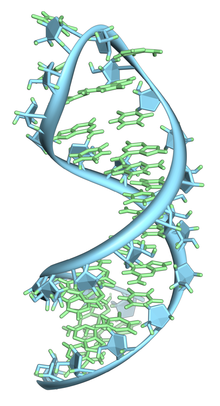
\includegraphics[width=2cm, height=4cm]{pictures/Pre-mRNA-1ysv-tubes.png}
\caption{
یک حلقه از pre-mRNA. نوکلئوبازها (سبز) و ستون فقرات ریبوز فسفات (آبی) مشخص شده اند. این یک رشته منفرد از آر‌ان‌ای است که بر روی خود تا می شود. عکس گرفته شده از ویکی‌پدیا
}\label{wrap-fig:1}
\end{wrapfigure}
نونوکلئوتیدها، مولکول‌های آلی شامل نوکلئوزید و فسفات می باشند. آن ها به عنوان واحدهای مونومری، پلیمرهای نوکلئیک اسیدی: دئوکسی ریبونوکلئیک اسید (دی‌ان‌ای) و ریبونوکلئیک اسید (آر‌ان‌ای) را تشکیل می‌دهند، که هردو مولکول‌های زیستی اساسی در تمام اشکال حیات روی زمین می باشند. نوکلئوتیدها از طریق رژیم غذایی به دست آمده و هم‌چنین در کبد از طریق مواد غذایی رایج سنتز می‌گردند.\cite{Nucleotide}

نوکلئوتیدها از سه زیر واحد مولکولی تشکیل شده اند: یک باز نوکلئوتیدی، یک قند پنج کربنه پنتوز (ریبوز یا دئوکسی ریبوز)، و یک گروه فسفات شامل یک تا سه فسفات. چهار باز نوکلئوتیدی دی‌ان‌ای شامل: گوانین، آدنین، سیتوزین و تیمین می باشند؛ در آر‌ان‌ای، اوراسیل به جای تیمین استفاده می‌گردد.

\section{آر‌ان‌ای}

اسید ریبونوکلئیک\LTRfootnote{\lr{RiboNucleic Acid}} یا آر‌ان‌ای
 یک مولکول پلیمری است که در نقش‌های بیولوژیکی مختلف مانند کدگذاری، رمزگشایی، تنظیم و بیان ژن‌ها ضروری است. آر‌ان‌ای به صورت یک رشته منفرد از نوکلئوتیدها (بازهای نیتروژنی گوانین، اوراسیل، آدنین و سیتوزین که با حروف G، U، A و C مشخص می شوند) است که برخودش پیچ می خورد، بر خلاف دی‌ان‌ای که با یک رشته دیگر جفت شده است.
 
نوعی از آر‌ان‌ای اطلاعات را از دی‌ان‌ای به سیتوپلاسم حمل می‌کند؛ به این نوع آر‌ان‌ای که اطلاعات را از دی‌ان‌ای به ریبوزوم‌ها حمل می‌کند، آر‌ان‌ای پیک یا پیامبر(mRNA) می‌گویند. نوعی دیگر از آر‌ان‌ای،
آر‌ان‌ای
 حامل (tRNA) است که اسیدهای آمینه را به ریبوزوم منتقل می‌کند، تا ریبوزوم، اسیدهای آمینه را بر اساس اطلاعات موجود در mRNA کنار یک دیگر قرار دهد. نوع دیگر، آر‌ان‌ای ریبوزومی (rRNA) است که در ساختار ریبوزوم‌ها شرکت دارد؛ این موضوع به این معناست که ریبوزوم (رناتن) ها متشکل از پروتئین ها و آر‌ان‌ای های ریبوزومی هستند.
\section{دی‌ان‌ای}

دئوکسی ریبو نوکلئیک اسید\LTRfootnote{\lr{Deoxyribonucleic acid}} به اختصار دی‌اِن‌اِی یک مولکول متشکل از دو زنجیره پلی نوکلئوتیدی است که به دور یکدیگر می‌پیچند و دارای دستورالعمل‌های ژنتیکی است که برای کارکرد و توسعهٔ زیستی جانداران و ویروس‌ها مورد استفاده قرار می‌گیرد. نقش اصلی مولکول دی‌ان‌ای ذخیره‌سازی طولانی مدت اطلاعات ژنتیکی و دستوری است. لیپید‌ها، پروتئین‌ها، کربوهیدرات های پیچیده (پلی ساکاریدها) و اسیدهای نوکلئیک، چهار درشت‌مولکول‌های اصلی و ضروری برای همه اشکال شناخته شده حیات هستند.

دو رشته دی‌ان‌ای به عنوان پلی نوکلئوتید شناخته می شوند زیرا از واحدهای مونومر یا تکپار ساده‌تری به نام نوکلئوتید تشکیل شده اند. هر نوکلئوتید از یکی از چهار نوکلئوباز حاوی نیتروژن ( سیتوزین C، گوانین G، آدنین A یا تیمین T )،  کربوهیدرات پنج‌کربنه به نام دئوکسی ریبوز و یک گروه فسفات تشکیل شده است. نوکلئوتیدها در یک زنجیره، توسط پیوندهای کووالانسی (معروف به پیوند فسفو دی استر) بین قند یک نوکلئوتید و فسفات نوکلئوتید بعدی به یکدیگر متصل می‌شوند و در نتیجه یک ستون فقرات قند-فسفات متناوب ایجاد می شود.
\begin{wrapfigure}{l}{6.5cm}
\centering
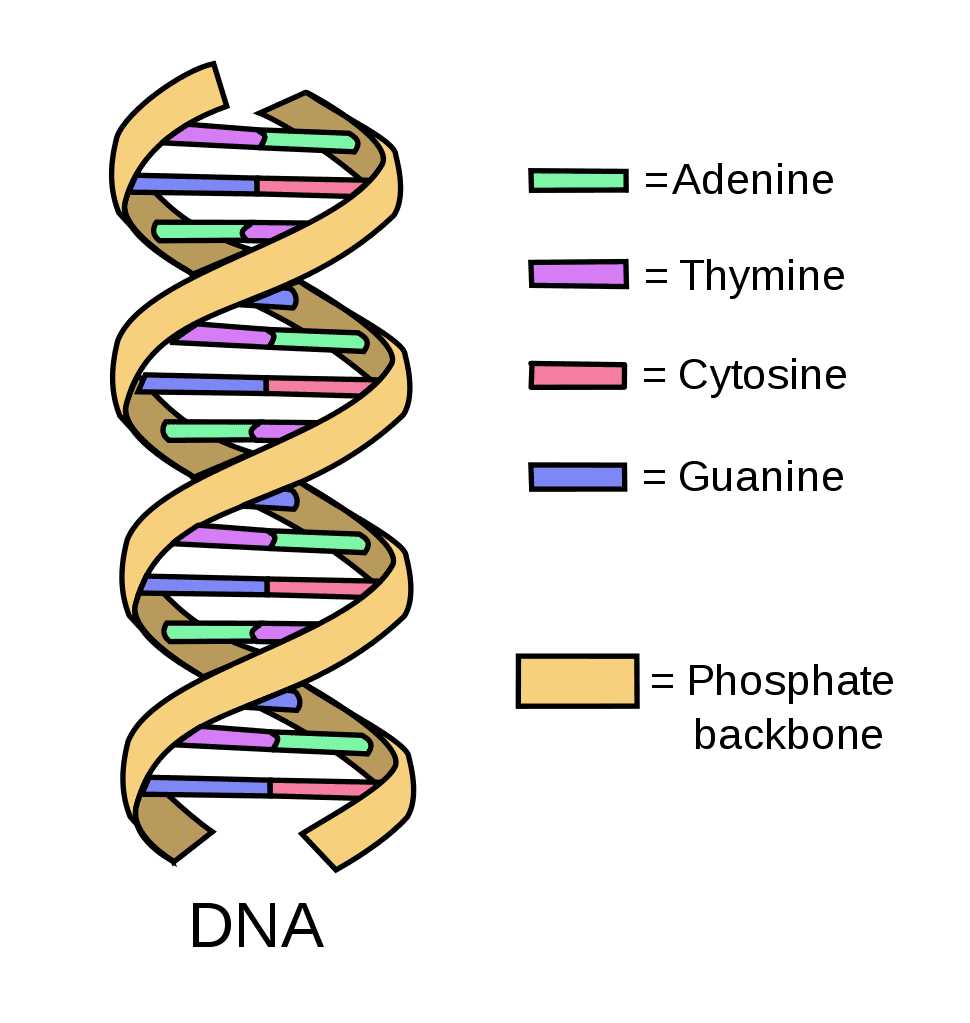
\includegraphics[width=4cm, height=5cm]{pictures/DNApng.png}
\caption{
شکل دو بعدی دی‌ان‌ای \cite{graph1}
}\label{wrap-fig:2}
\end{wrapfigure}
 بازهای نیتروژنی، دو رشته پلی نوکلئوتیدی جداگانه، طبق قوانین جفت شدن باز‌ها 
\lr{)}A با T و C با G\lr{(}
، با پیوندهای هیدروژنی به یکدیگر متصل می شوند تا دی‌ان‌ای دو رشته‌ای بسازند. این دو رشته مکمل، ناهمسو و محلول (در آب) هستند (دی‌ان‌ای حلقوی قطبیت ندارد اما هر رشته از دی‌ان‌ای خطی دارای قطبیت است). بازهای نیتروژنی مکمل به دو گروه پیریمیدین‌ها و پورین‌ها تقسیم می شوند. در دی‌ان‌ای، پیریمیدین ها تیمین و سیتوزین هستند. پورین‌ها آدنین و گوانین هستند.


هر دو رشته دی‌ان‌ای اطلاعات بیولوژیکی یکسانی را ذخیره می‌کنند. این اطلاعات زمانی که دو رشته از هم جدا می‌شوند، تکرار می شوند. بخش بزرگی از دی‌ان‌ای (بیش از 98٪ برای انسان) کد نشده\LTRfootnote{\lr{non-coding}}
 است، به این معنی که این بخش‌ها، توالی‌های پروتئین را کد نمی‌کنند. دو رشته دی‌ان‌ای در جهت مخالف یکدیگر قرار دارند و بنابراین باز مکمل ابتدای یک رشته، آخر رشته دیگر هستند. در آیین نامگذاری ترکیبهای شیمیایی، اتمهای کربن در حلقهٔ شکری نوکلئوتید شماره‌گذاری شده‌اند. هر رشتهٔ دی‌ان‌ای یا آران‌ای دارای یک پایانهٔ '۵ که معمولا شامل یک گروه فسفاتی است و یک پایانهٔ '۳ که معمولاً از جانشین ریبوز اصلاح نشده -OH است. به هر قند یکی از چهار نوع نوکلئوباز (یا باز) متصل است. توالی این چهار هسته در امتداد ستون فقرات است که اطلاعات ژنتیکی را رمزگذاری می کند. رشته‌های آر‌ان‌ای با استفاده از رشته‌های دی‌ان‌ای به‌عنوان یک الگو در فرآیندی به نام رونویسی ایجاد می‌شوند که در آن بازهای دی‌ان‌ای با بازهای مربوطه خود مبادله می‌شوند، به جز در مورد تیمین (T)، که آر‌ان‌ای جایگزین اوراسیل (U) می‌شود. تحت کد ژنتیکی، این رشته‌های آر‌ان‌ای توالی اسیدهای آمینه درون پروتئین‌ها را در فرآیندی به نام "ترجمه`` مشخص می‌کنند.
\subsection{تفاوت‌های دی‌ان‌ای و آران‌ای}
\begin{wrapfigure}[4]{l}{0.4\textwidth}
\centering
\vspace{-45pt}
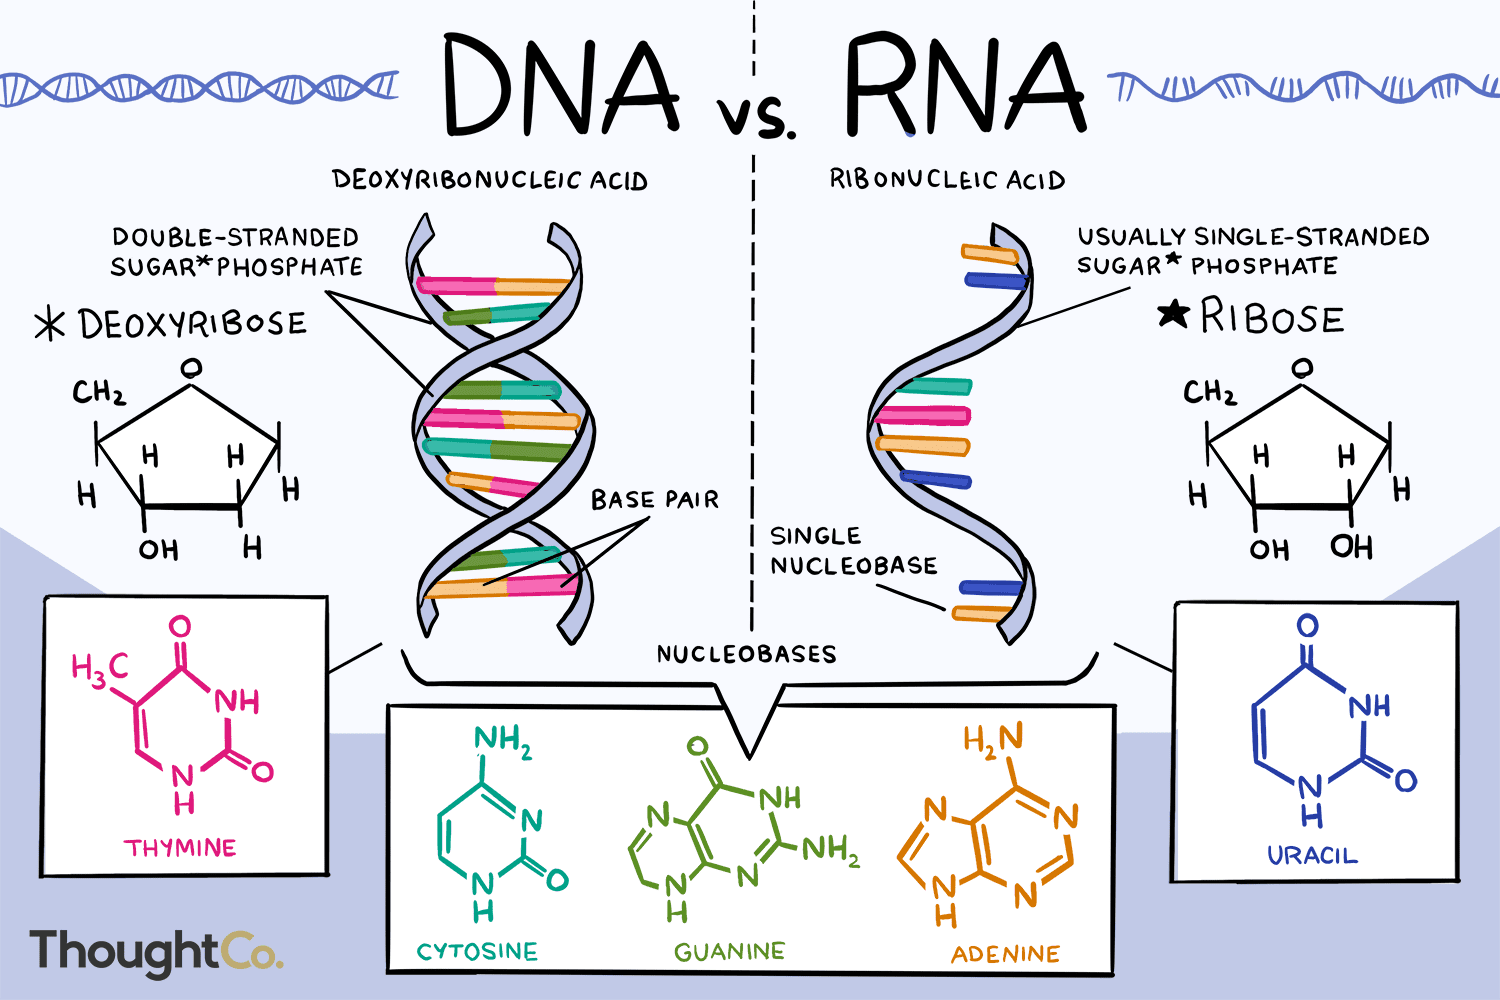
\includegraphics[width=0.4\textwidth]{pictures/dnarna.png}
\caption{
مقایسه دی‌ان‌ای و آران‌ای \cite{graph2}
}\label{wrap-fig:3}
\end{wrapfigure}
تفاوت‌ها:
\begin{itemize}
\item دی‌ان‌ای برعکس آر‌ان‌ای از هستهٔ سلول خارج نمی‌شود.
\item آر‌ان‌ای بدون ژن می‌باشد.
\item دی‌ان‌ای در ذخیره و آر‌ان‌ای در انتقال اطلاعات وراثتی و در ساختار ریبوزوم نقش دارد.
\item مولکول دی‌ان‌ای دو رشته‌ای در هم تنیده اما مولکول آر‌ان‌ای تک‌رشته‌ای است.
\end{itemize}
\newpage
\begin{itemize}
\item 
در دی‌ان‌ای باز آلی یوراسیل و در آر‌ان‌ای باز آلی تیمین شرکت ندارد ( U در دی‌ان‌ای و T در آر‌ان‌ای ).
\item
قند پنج‌کربنه موجود در دی‌ان‌ای را دئوکسی ریبوز و در آر‌ان‌ای قند ریبوز نامیده می شود. تفاوت بین قندها وجود گروه هیدروکسیل بر روی کربن '۲ ریبوز و عدم وجود آن در کربن '۲ دئوکسی ریبوز است.

\end{itemize}
شباهت‌ها:
\begin{itemize}
\item هر دو پلیمر هستند و از نوکلئوتید تشکیل شده‌اند.
\item در هر دو نوکلئوتیدهای مقابل با پیوند هیدروژنی و نوکلئوتیدهای کناری با پیوند فسفو دی‌استر به هم متصل می‌شوند (گاهی نوکلئوتیدهای دو بخش متفاوت از یک رشته آران‌ای، به هم متصل می‌شوند).
\item نوکلئوتیدهای آزاد (واحدهای سازنده آزاد) هر دو مولکول پیش از اتصال سه فسفات بوده و با اتصال به رشته پلی‌نوکلئوتیدی تک‌فسفاته می‌شوند.

\end{itemize}


\section{ویرایش ژنوم}
\begin{wrapfigure}[14]{l}{0.5\textwidth}
\centering
\vspace{-65pt}
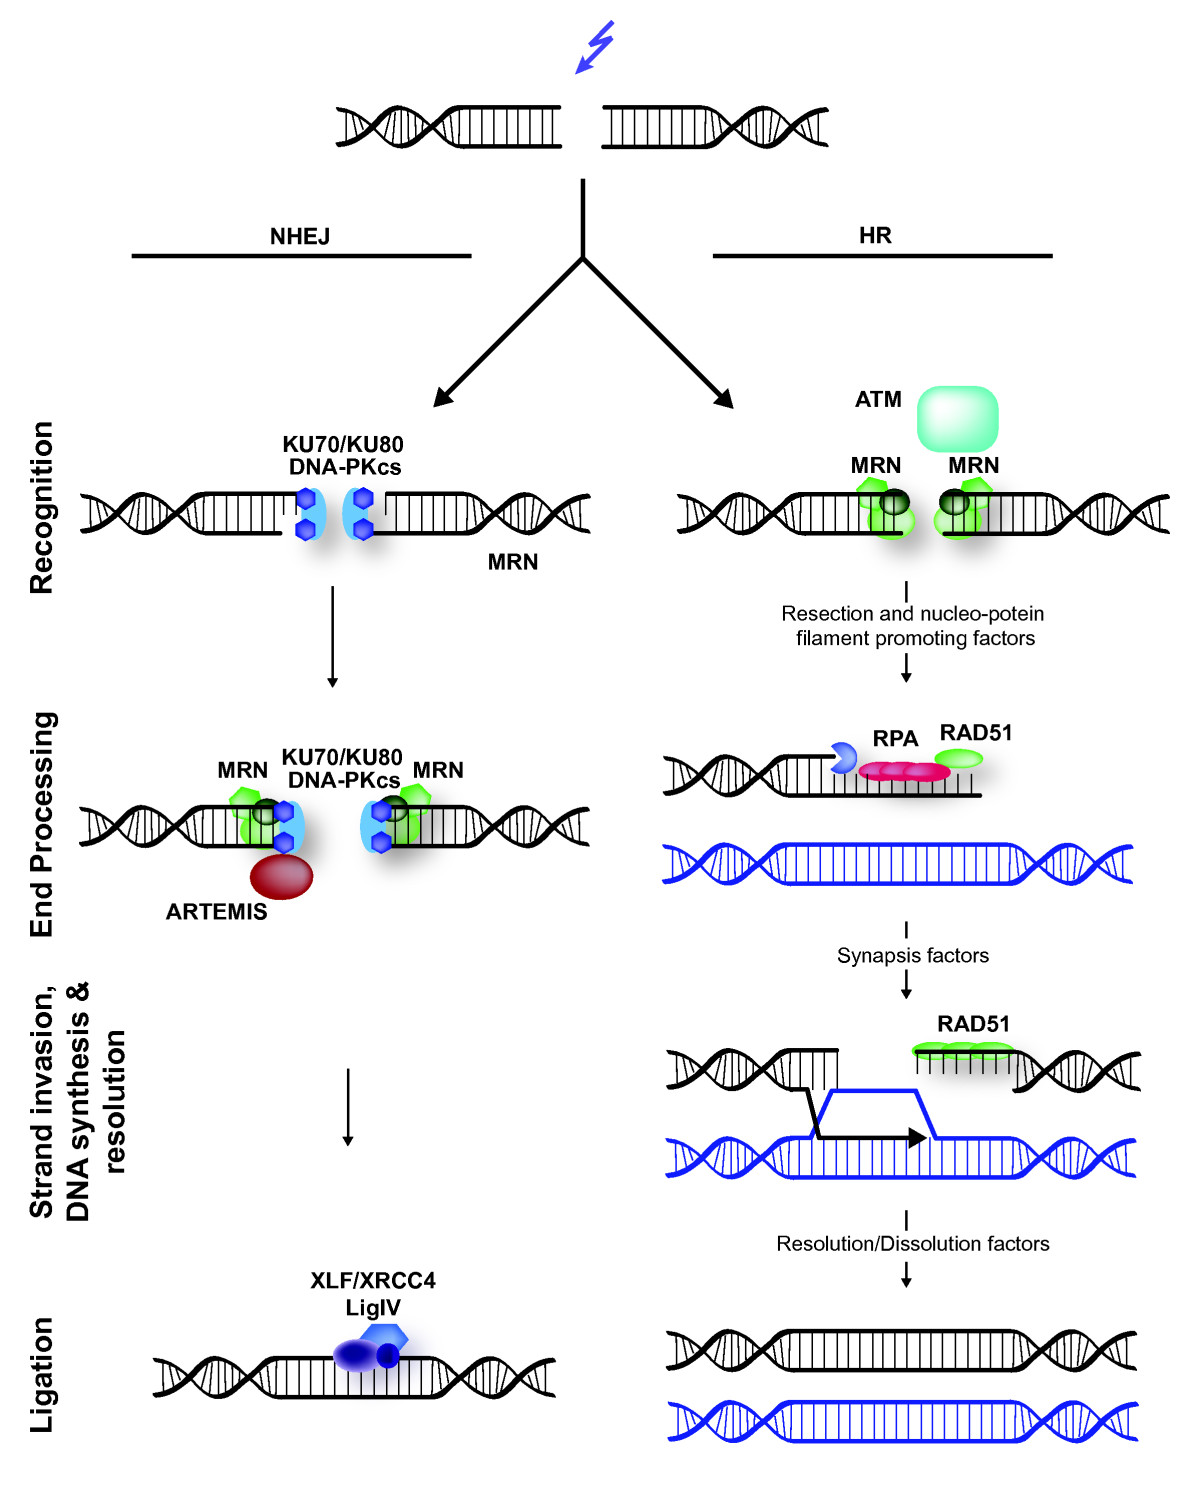
\includegraphics[width=8cm, ]{pictures/DBSrepair.jpg}
\vspace{-15pt}
\caption{
مکانیزم ترمیم دی‌ان‌ای، عکس گرفته شده از ویکی‌پدیا.
}\label{wrap-fig:4}
\end{wrapfigure}
مهندسی ژنوم یا ویرایش ژنوم نوعی از مهندسی ژنتیک است که در آن دی‌ان‌ای ژنوم یک موجود زنده حذف، اضافه، اصلاح یا جایگزین می‌شود. در دهه ۱۹۶۰، دانشمندان با شارش پرتو‌های رادیواکتیو بر روی گیاهان به تغییر تصادفی   بر روی ژنوم‌ دست یافتند. این کار به هدف رسیدن به یک تغییر ژنتیک مفید صورت می‌گرفت و البته نتابج خوبی هم به همراه داشت ولی با این حال راندمان پایین این ویرایش‌ها باعث شد که دانشمندان به فکر راه‌های دیگری برای ویرایش ژنوم باشند.

تا کنون سه تکنیک موفق و معروف برای ویرایش ژنوم مهندسی شده است:
 نوکلئاز انگشت روی\LTRfootnote{\lr{Zinc Finger Nuclease}} 
\lr{(ZFNs)}
، نوکلئازهای اثرگذار شبه فعال کننده رونویسی\LTRfootnote{\lr{Transcription activator-like effector nuclease}} 
\lr{(TALEN)}
، و سیستم تناوب‌هایِ کوتاهِ پالیندرومِ فاصله‌دارِ منظمِ خوشه‌ای\LTRfootnote{\lr{Clustered Regularly Interspaced Short Palindromic Repeats}}
\lr{(CRISPR)}. 
کلید ویرایش ژنوم ایجاد شکست دو رشته‌ی دی‌ان‌ای در نقطه مورد نظر است و این سه روش مبتنی بر شکست درست دی‌ان‌ای در نقطه مورد نظر مهندسی شدند.
\subsection{ شکست و تعمیر دی‌ان‌ای}
شکل رایج ویرایش ژنوم بر مفهوم مکانیک ترمیم شکست دو رشته‌ای دی‌ان‌ای
\LTRfootnote{\lr{Double-Strand Break (Cut)}}\lr{(DSB)}
تکیه دارد. دو مسیر اصلی وجود دارد که DSB را تعمیر می‌کند. اتصال انتهای غیر همولوگ
\LTRfootnote{\lr{Non-Homologous End Joining}}
 \lr{(NHEJ)}
  و تعمیر هدایت شده همولوژی
 \LTRfootnote{\lr{Homology Directed Repair}}
   \lr{(HDR)}. NHEJ از انواع آنزیم‌ها برای اتصال مستقیم به انتهای دی‌ان‌ای استفاده می‌کند، در حالی که HDR دقیق‌تر از یک توالی همولوگ به عنوان الگویی برای بازسازی توالی‌های دی‌ان‌ای گمشده در نقطه شکست استفاده می‌کند. این را می توان با ایجاد یک بردار با عناصر ژنتیکی مورد نظر در یک توالی که همولوگ با توالی های کناری یک DSB است مورد استفاده قرار داد. این باعث می شود که تغییر مورد نظر در محل DSB درج شود. در حالی که ویرایش ژن مبتنی بر HDR مشابه هدف‌گیری ژن مبتنی بر نوترکیب همولوگ است، نرخ نوترکیبی حداقل سه مرتبه افزایش می‌یابد.
\subsubsection{NHEJ}

پرتوهای یونیزه کننده و برخی داروهای ضد سرطان باعث شکست هر دو رشته ی دی‌ان‌ای می شوند .سیستمی که برای ترمیم این نوع آسیب به کار گرفته میشود، سیستم ترمیم اتصال انتهای غیر همولوگ (NHEJ) میباشد که مستعد به خطا به شمار می رود، زیرا همواره چندین نوکلئوتید در جایگاه ترمیم از بین می روند و دو انتهای شکسته شده از کروموزوم های همولوگ یا غیر همولوگ به یکدیگر متصل می شوند.
زمانی که کروماتیدهای خواهری برای ترمیم شکست های دو رشته ای در دسترس نباشند این نوع ترمیم صورت میگیرد . در ابتدا کمپلکسی از ku70/80 و پروتئین کیناز وابسته به دی‌ان‌ای به انتهاهای شکسته دو رشته اتصال می یابند، آن گاه در هر انتها چندین باز توسط نوکئاز حذف شده و دو مولکول از طریق آنزیم لیگاز به هم متصل می گردند. 
\lr{DSB}ها
 ترجیحاً در سلول، توسط اتصال انتهایی غیر همولوگ (NHEJ) ترمیم می شوند، مکانیزم سریعی که اغلب باعث درج یا حذف (indels) در دی‌ان‌ای می شود. ایندل ها اغلب منجر به تغییر اساسی در دی‌ان‌ای می شوند، به‌طوری که دی‌ان‌ای عملکرد خود را از دست می دهند. پس در نتیجه معمولا به عنوان سلول مرده درنظر گرفته می‌شوند و حذف می‌شوند. برای ویرایش ژنوم مطمئن، اعمال شدن ویرایش و تغییر نکردن آن نکات مهمی است. پس دانشمندان تمام تلاششان را می‌کنند که بعد از DBS، دی‌ان‌ای به این روش تعمیر نشود.
\subsubsection{HDR}
 تعمیر هدایت شده همولوژی (HDR)، مکانیزمی در سلول ها برای ترمیم ضایعات دی‌ان‌ای دو رشته‌ای، از یک نسخه مشابه دی‌ان‌ای برای ترمیم استفاده می کند. رایج ترین شکل HDR، نوترکیبی همولوگ است. مکانیسم HDR تنها زمانی می تواند توسط سلول استفاده شود که یک قطعه همولوگ از دی‌ان‌ای در هسته وجود داشته باشد، عمدتاً در فاز G2 و S چرخه سلولی. نمونه‌های دیگر تعمیر مبتنی بر HDR شامل تعمیر تک رشته‌ای و تکثیر ناشی از شکستگی است. هنگامی که دی‌ان‌ای همولوگ وجود ندارد، فرآیند NHEJ به جای آن انجام می‌شود.

\subsection{\lr{Zinc finger nucleases (ZFN)}}

نوکلئاز انگشت روی یا ZFN اولین سیستم پروتئینی متصل شونده به دی‌ان‌ای قابل برنامه ریزی با کاربرد وسیع است.ZFNها شامل زنجیره ای از پروتئین های انگشت روی هستند که به یک نوکلئاز باکتریایی ملحق شده اند تا بتوانند سیستمی را تولید کنند که قادر به ایجاد برش های دو رشته ای خاص در دی‌ان‌ای برای ویرایش ژن باشد. پروتئین های انگشت روی هدف قرار دادن ناحیه خاص را فراهم می کنند زیرا هر یک از آنها سه جفت باز یا ۳bp از دی‌ان‌ای را شناسایی می کنند. نوکلئازی که معمولاً در تکنولوژی ZFN متصل به زنجیره پروتئین های انگشت روی است FokI نام دارد که برای اتصال به دی‌ان‌ای باید دایمریزه شده باشد، بنابراین یک جفت از ZFN برای هدف گیری و برش دی‌ان‌ای مورد استفاده قرار می گیرد.این آنزیم ها کمک زیادی به تولید موجودات ترانسژنیک می کنند و بدلیل اینکه فراوانی نوترکیبی همولوگ بسیار ناچیز بوده، اهمیت زیادی در مهندسی ژنتیک و مطالعات ترانسژنیک ، ناک اوت و غیره پیدا کرده اند. این پروتئین های مهندسی شده و متصل شونده به دی‌ان‌ای می توانند ژنوم را در جایگاه های ویژه‌ای شناسایی کرده و ایجاد برش های دو رشته‌ای کنند . در صورتی که سیستم تعمير NHEJ فعال شود چون این سیستم ترمیم مستعد خطاست، سبب ایجاد جهش در آن ناحیه خاص از ژنوم می شود بنابراین در مطالعات موتاژنز نیز اهمیت دارند. انتقال یک بردار حاوی ژن مورد نظر به همراه ZFNs سبب تسهیل درج ژن در آن ناحیه از ژنوم می گردد.

\subsection{TALEN}
\begin{wrapfigure}{l}{8cm}
\centering
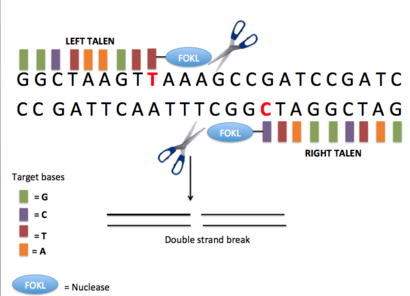
\includegraphics[width=6cm, ]{pictures/Overview_of_TALENs.png}
\caption{
مکانیزم TALEN \cite{graph3}
}\label{wrap-fig:4}
\end{wrapfigure}
نوکلئازهای رونویس مؤثر-مانند فعال‌کننده
\footnote{\lr{Transcription activator-like effector nucleases}} \lr{(TALENs)}
 پپروتئین های متصل شونده به دی‌ان‌ای با آرایه تکراری 33 یا 34 اسید آمینه هستند.
\lr{TALEN}
ها آنزیم های محدودکننده مصنوعی هستند که از ادغام حوزه برش دی‌ان‌ای یک نوکلئاز با دامنه های TALE طراحی شده اند، که می توانند به طور خاص یک توالی دی‌ان‌ای منحصر به فرد را شناسایی کنند. این پروتئین‌های ادغام شده به‌عنوان قیچی دی‌ان‌ای برای ویرایش یک ژن خاص عمل می‌کنند که به‌ راحتی قابل برنامه‌نویسی بوده و قادر به انجام تغییرات هدفمند ژنوم مانند درج توالی، حذف، تعمیر و جایگزینی در سلول‌های زنده هستند.\cite{TALEN1} این تکنولوژی را می‌توان برای تغییر هر نقطه از دی‌ان‌ای استفاده کرد.
 \lr{TAL‌E}،های
 یک رشته ۳۴تایی از آمینو‌اسید‌ها هستند که هر کدام وظیفه دارند که یک تک نوکلئوتید را پیدا کنند. نوکلئاز می‌تواند شکستگی‌های دو رشته‌ای را در محل هدف ایجاد کند، که قادر است با اتصال انتهایی غیر همولوگ (NHEJ) ترمیم شود، که منجر به اختلالات ژنی از طریق وارد کردن یا حذف‌های تک نوکلوتیدی می شود، هر تکرار حفظ می شود. به استثنای دی باقیمانده متغیر تکرار شونده
\footnote{\lr{Repeat Variable Di-residues}}(RVDs)،
 که در موقعیت‌های آمینواسید 12 و 13 قرار دارند. RVD ها توالی دی‌ان‌ای را تعیین می کنند که TALE به آن متصل می شود. این تناظر ساده یک به یک بین تکرارهای TALE و توالی دی‌ان‌ای مربوطه باعث می‌شود روند مونتاژ آرایه‌های تکراری برای تشخیص توالی‌های دی‌ان‌ای جدید، ساده باشد. این 
\lr{TALE}ها
 را می توان با کاتالیزوری از یک نوکلئاز از دی‌ان‌ای به نام 
\lr{FokI}
، ادغام کرد تا با آن TALENها را ساخت. ساختارهای TALEN توالی‌های دی‌ان‌ای را فقط در مکان‌های از پیش انتخاب شده متصل می‌کنند و می‌شکنند. هدف TALEN را می توان بر اساس یک کد آسان پیش بینی کرد. با توجه به این که محل اتصال بیش از ۳۰ جفت نوکلئوتید است، نوکلئازهای TAL مختص هدفی یکتا هستند. هر نوکلئوتید منفرد در ژنوم در صورتی که در محدوده 6 جفت نوکلئوتید باشد، TALEN می‌تواند آن را ویرایش کند.
سازه های TALEN به روشی مشابه با نوکلئازهای انگشت روی طراحی شده استفاده می‌شوند و دارای سه مزیت در جهش زایی هدفمند هستند: (1) احتمال ویرایش درست هدف بالاتر است، (2) اثرات خارج از هدف کمتر است و (3) طراحی آن آسان تر است.\cite{TALEN2}
\section{کریسپر}
 \lr{Clustered Regularly Interspaced Short Palindromic Repeats}
 یا به اختصار کریسپر (به انگلیسی: CRISPR ) به معنی "تناوب‌هایِ کوتاهِ پالیندرومِ فاصله‌دارِ منظمِ خوشه‌ای`` بخشی از دی‌ان‌ای پروکاریوت هستند که حاوی تناوب‌های کوتاهِ توالی‌های بنیادین هستند. بخشی از سیستم کریسپر "پروتئین Cas9 `` است. این پروتئین قابلیت جستجو، برش زدن و تغییر دی‌ان‌ای را دارد. قبل از این تکنیک از روش "تحویل یا انتقال ژن" استفاده می‌شد، به این صورت که از یک ناقل ویروسی یا غیرویروسی برای انتقال ژن سالم به ژنوم سلول میزبان استفاده می‌شد، ولی در روش کریسپر، ژن معیوب برش داده می‌شود و ژن سالم به جای آن قرار می‌گیرد. استفاده از آنزیم Cas9 خطر کمتری نسبت به روش قبلی که یک ژن خارجی وارد ژنوم می‌شد دارد، زیرا گاهی ژن خارجی به سرطان منجر می‌شود اما ژنی که از طریق کریسپر ترمیم شود کنترل شده است. نام دیگر این تکنیک "قیچی ژنتیکی" است که به دلیل ساز و کار آنزیم "کَس9" (Cas9) هست. این آنزیم به عنوان یک جفت قیچی مولکولی می‌تواند دو رشته دی‌ان‌ای را در محل خاصی از ژنوم برش دهد.\cite{TED}
\begin{figure}[!h]
\centering
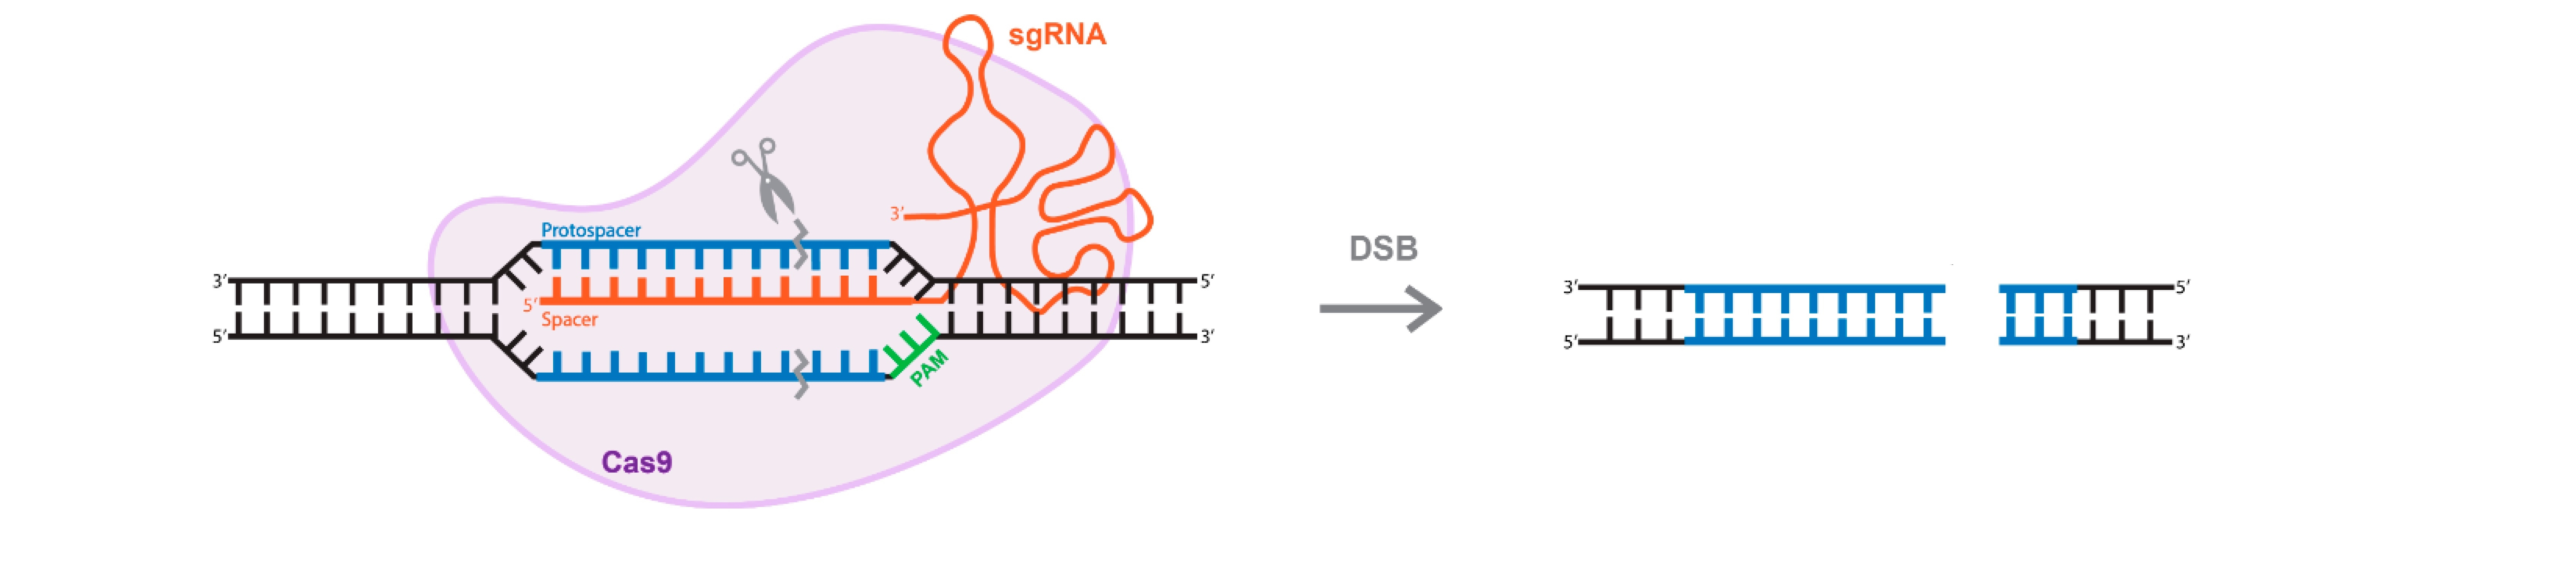
\includegraphics[width=15cm, ]{pictures/simple_crispr.jpg}
\caption{
مکانیزم ساده شده‌ای از CRISPR \cite{graph4}
}\label{fig:1}
\end{figure}

\subsection{کریسپر در باکتری}

اولین بار سیستم کریسپر در
 \lr{Escherichia coli}
 به عنوان یک توالی تکراری ۲۹ نوکلئوتیدی با فاصله ۳۲ نوکلئوتیدی توسط یوشیزومی ایشی نو ژاپنی در سال ۱۹۸۷ مطرح شد که باکتری‌ها و آرکی باکتری‌ها را از حمله باکتریوفاژها و پلاسمیدها محافظت می‌کند. این سیستم‌های دفاعی به یک آر‌ان‌ای کوچک شناساگر توالی خاص تکیه می‌کنند و اسیدهای نوکلئیک خارجی را خاموش می‌کنند.
\cite{Ishino} \lr{Francisco Mojica}
 و همکارانش در سال ۱۹۹۳ تکرارهای مشابهی را در چندین گونه میکروبی دیگر یافتند.\cite{Mojica}
بعد از حمله به سلول توسط عناصر ژنتیکی خارجی مانند باکتریوفاژها یا پلاسمیدها (مرحله ۱: تزریق فاژ)، آنزیم‌های ویژه مرتبط CRISPR
 به نام
 \lr{Cas (CRISPR-associated protein)}
 توالی‌های spacer را از توالی‌های protospacer جدا کرده و آن‌ها را به درون لوکوس‌های کریسپر موجود در ژنوم پروکاریوت‌ها وارد و متصل می‌کنند. ( مرحله ۲: استفاده از spacer ). این 
\lr{spacer}ها
 بین تکرارهای مستقیم تقسیم شده‌اند که اجازه می‌دهند سیستم CRISPR ، به‌طور ایمن و دقیق و نه به‌طور غیر ایمن، شناسایی شود. آرایهٔ CRISPR یک رونوشت آر‌ان‌ای غیر کدونی است که از نظر آنزیمی از طریق مسیرهای متمایز که برای هر نوع سیستم CRISPR منحصر به فرد است، بالغ می‌شود. ( مرحله ۳: بیوژنز و پرادازش CrRNA ) در CRISPR نوع I و
 \lr{،III} 
رونوشت pre-CrRNA توسط ریبونوکلئازهای مرتبط با CRISPR ، شکسته می‌شوند و این کار موجب آزاد شدن چندین CrRNAs کوچک می‌شود. به‌طور متوسط CrRNA نوع III بیشتر در انتهای ´۳ توسط
 \lr{RNase}هایی 
که هنوز مشخص نشده‌اند برای تولید رونوشت کاملاً بالغ پردازش می‌شوند. CRISPR نوعII، یک آر‌ان‌ای کریسپر فعال‌کننده ترانس است (tracrRNA) که با تکرارهای مستقیم هیبرید می‌شود و یک آر‌ان‌ای دوپلکس را تشکیل می‌دهد و توسط 
\lr{RNase III}
 درونی و نوکلئازهای ناشناخته دیگر شکسته و پردازش می‌شود. CrRNA های بالغ شده نوع I و III سیستم CRISPR ، سپس درون افکتورهای کمپلکس‌های پروتئینی برای تشخیص و تخریب توالی هدف اضافه می‌شوند. در سیستم‌های نوع II، کمپلکس هیبرید CrRNA-tracrRNA به Cas9 متصل شده و در واقع هیبرید شدن این دو باعث فعال شدن Cas9 می‌شود. هر دو نوع I و III سیستم CRISPR از چند پروتئین مداخله گر تنظیم‌کننده برای تسهیل شناسایی توالی هدف استفاده می‌کنند. در CRISPR نوعI، کمپلکس Cascade با یک مولکول CrRNA لود می‌شود که یک مجموعه نظارتی بی نظیری است که دی‌ان‌ای هدف را شناسایی می‌کند. سپس نوکلئازCas3، لوپ \lr{R Cascade} را به کار گرفته و به آن متصل می‌شود و واسطه تخریب توالی هدف می‌شود. در CRISPR نوع \lr{III, CrRNA}ها یا به کمپلکس‌های Csm یا به کمپلکس‌های Cmr به ترتیب متصل شده و به ترتیب سوبستراهای دی‌ان‌ای و RNA را می‌شکنند. درمقابل، سیستم نوع II فقط نیاز به Cas9 برای تخریب دی‌ان‌ای جفت شده با آر‌ان‌ای راهنما دوپلکس خود دارد که این آر‌ان‌ای راهنما حاوی ترکیبی از CrRNA-tracrRNA است.
\subsection{عمل کرد کریسپر در ژن}
همانطور که گفتیم، مدل‌های مختلفی از CRISPR تا به حال درست شده است ولی به صورت کلی می‌توان CRISPR را به دو قسمت آر‌ان‌ای و  cas تقسیم کرد که cas در آن وظیفه جدا کردن دو رشته دی‌ان‌ای را از هم دارد و آر‌ان‌ای که هدف را مشخص و قیچی می‌کند. برای این که دقیقا نقطه شکست دی‌ان‌ای مشخص شود، cas نیاز به یک علامت دارد که با رسیدن به آن کار خود را شروع کند. به این رشته PAM یا 
\lr{Protospacer Adjacent Motif}
گفته می‌شود که کاملا وابسته به cas است. همان طور که از قبل گفتیم بعد از شکست دی‌ان‌ای، دو مکانیزم برای تعمیر آن وجود دارد. دانشمندان تکنولوژی‌های CRISPR مختلفی را برای افزایش احتمال تعمیر HDR ایجاد کرده‌اند که هر یک ویژگی‌های خاص خود را دارند ولی ما در پژوهش خود ساده‌ترین مورد آن یعنی cas9 به همراه یک آر‌ان‌ای که به آن sgRNA یا 
\lr{single guide RNA}
می گویند، استفاده کرده‌ایم. این طرح باعث محدود شدن هدف‌های مورد استفاده می‌شود به طوری که ‌PAM باید به شکل NGG باشد که در آن N یک نوکلیوتید دلخواه است. در نتیجه رشته هدف همیشه با NGG ختم می‌شود. 
\begin{figure}[!h]
\centering
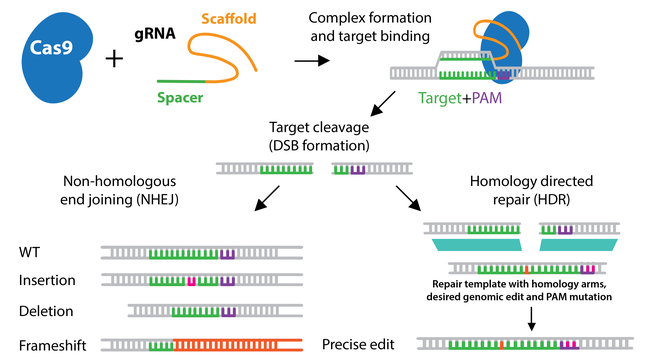
\includegraphics[width=10cm, ]{pictures/cut.png}
\caption{
مکانیزم CRISPR \cite{addgene}
}\label{fig:2}
\end{figure}
 
\subsection{حساسیت}
حساسیت در یک طرح CRISPR میزان اختصاصی بودن توالی هدف گیری شده توسط gRNA در مقایسه با بقیه ژنوم تعیین می شود. در حالت ایده‌آل، یک توالی هدف‌گیری شده توسط gRNA ، همسانی کاملی با دی‌ان‌ای هدف خواهد داشت و هیچ همسانی در جای دیگری در ژنوم وجود ندارد یعنی دقیقا هدف را ویرایش می‌کند، نه جای دیگری را. با این حال، به طور واقع بینانه، یک توالی که با gRNA هدف قرار گرفته شده، مکان‌های بیشتری را، در سراسر ژنوم ویرایش خواهد داد که در آن همولوژی نسبی وجود دارد. این ناحیه‌ها خارج از هدف یا offtarget نامیده می شوند و باید هنگام طراحی یک gRNA برای آزمایش خود در نظر گرفته شوند.

علاوه بر بهینه سازی طراحی gRNA ، حساسیت CRISPR نیز می تواند از طریق تغییرات در Cas9 افزایش یابد. همانطور که قبلاً بحث شد، Cas9 از طریق فعالیت ترکیبی دو حوزه نوکلئاز، RuvC و HNH ، شکست‌های دو رشته ای (DSBs) ایجاد می کند. نیکاز Cas9 ، یک جهش D10A از SpCas9 ، یک دامنه نوکلئاز را حفظ می‌کند و به جای  DSB، یک دی‌ان‌ای نیک تولید می کند.

بنابراین، دو نیکاز که رشته‌های دی‌ان‌ای مخالف را هدف قرار می دهند، برای تولید DSB در دی‌ان‌ای هدف مورد نیاز است. این نیاز برای یک سیستم CRISPR نیکاز دوتایی یا نیکاز دوگانه به طور چشمگیری ویژگی هدف را افزایش می‌دهد، زیرا بعید است که دو ناک خارج از هدف به اندازه کافی نزدیک به ایجاد DSB ایجاد شوند. اگر حساسیت بالا برای آزمایش شما بسیار مهم است، ممکن است استفاده از رویکرد نیکاز دوگانه را برای ایجاد یک DSB القا شده با نیک دوگانه در نظر بگیرید. سیستم نیکاز همچنین می تواند با ویرایش ژن با واسطه HDR برای ویرایش های ژنی خاص ترکیب شود.

در سال 2015، محققان از 
\lr{rational mutagenesis}
 برای توسعه دو Cas9 با ثبات بالا استفاده کردند:
\lr{eSpCas9} و\lr{SpCas9-HF1}.   
 \lr{eSpCas9} حاوی جایگزین‌های آلانین است که برهمکنش‌های بین شیار HNH/RuvC و رشته دی‌ان‌ای غیرهدف را تضعیف می‌کند و از جدا شدن رشته‌ها و برش در مکان‌های خارج از هدف جلوگیری می‌کند. به طور مشابه، SpCas9-HF1 ویرایش خارج از هدف را از طریق جایگزینی آلانین کاهش می دهد که برهمکنش Cas9 با ستون فقرات فسفات دی‌ان‌ای را مختل می کند. یکی دیگر از Cas9 با حساسیت بالا، HypaCas9، در سال 2017 توسعه یافت و حاوی جهش‌هایی در دامنه REC3 است که تصحیح Cas9 و تبعیض هدف را افزایش می‌دهد. 
هر سه آنزیم با حساسیت بالا نسبت به Cas9 نوع وحشی، ویرایش خارج از هدف کمتری تولید می کنند.

\subsection{تاثیرگذاری}
تاثیرگذاری در یک طرح CRISPR احتمال شکست دی‌ان‌ای و ویرایش درست را تعیین ‌می‌کند. برای غلبه بر راندمان پایین HDR، محققان دو دسته از ویرایشگرهای پایه را ایجاد کرده‌اند - ویرایشگرهای پایه سیتوزینی \lr{(CBEs)} و ویرایشگرهای پایه آدنین \lr{(ABEs)}.

ویرایشگرهای پایه سیتوزینی با ادغام نیکاز Cas9 یا Cas9 مرده غیرفعال کاتالیزوری \lr{(dCas9)} به سیتیدین دآمیناز مانند APOBEC ایجاد می‌شوند. ویرایشگرهای پایه توسط یک gRNA در یک مکان خاص قرار می‌گیرند و می توانند سیتیدین را در یک پنجره ویرایش کوچک در نزدیکی سایت PAM به یوریدین تبدیل کنند. اوریدین متعاقباً از طریق ترمیم برش پایه به تیمیدین تبدیل می‌شود و تغییر C به T (یا G به A در رشته مخالف) را ایجاد می‌کند.

به طور مشابه، ویرایشگرهای پایه آدنوزین برای تبدیل آدنوزین به اینوزین مهندسی شده‌اند، که سلول با آنها مانند گوانوزین رفتار می‌کند و تغییر A به G (یا T به \lr{(C} را ایجاد می‌کند. آدنین دی‌ان‌ای دآمینازها در طبیعت وجود ندارند، اما با تکامل هدایت شده \lr{Escherichia coli TadA}، یک tRNA آدنین دآمیناز ایجاد شده اند. مانند ویرایشگرهای پایه سیتوزین، دامنه تکامل یافته TadA با پروتئین Cas9 ترکیب می شود تا ویرایشگر پایه آدنین ایجاد شود.

هر دو نوع ویرایشگر پایه با چندین نوع Cas9 از جمله Cas9 با ثبات بالا در دسترس هستند. پیشرفت‌های بیشتری با بهینه‌سازی بیان پروتئین، اصلاح ناحیه پیوندی بین نوع Cas و دآمیناز برای تنظیم پنجره ویرایش، یا افزودن ترکیب‌هایی که خلوص محصول را افزایش می‌دهند مانند مهارکننده دی‌ان‌ای گلیکوزیلاز \lr{(UGI)} یا Gam مشتق از باکتریوفاژ \lr{(Mu-GAM)} انجام شده است.






\subsection{انواع کریسپر}
طبقه‌بندrova و همکاران ۵ نوع سیستم کریسپر را تعریف می‌کند که دارای ۱۶ زیر نوع بر اساس ویژگی‌های مشترک و شباهت تکاملی است. که به دو دسته بزرگ تقسیم می‌شوند. کلاس‌ها بر اساس ساختار پیچیده‌ای است که دی‌ان‌ای ژنوم را تجزیه می‌کند. نوع II CRISPR/Cas اولین سیستم برای مهندسی ژنوم، با نوع V در ۲۰۱۵ بود.

در گام بعدی از روی ژن‌های کمپلکس cas هم پروتئین Cas9 ساخته می‌شود. سپس کمپلکس Cas9-crRNA-tracrRNA تشکیل می‌شود؛ که این کمپلکس لازم و ضروری برای هدف قرار دادن یا تخریب دی‌ان‌ای خارجی می‌باشد.

\subsubsection{ Single-Strand Break (Nick)}
\begin{wrapfigure}{l}{8cm}
\centering
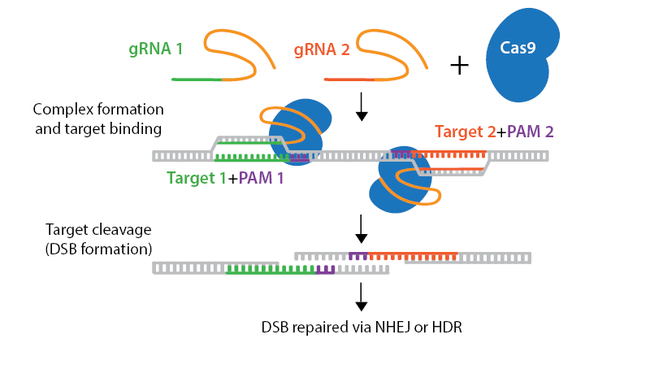
\includegraphics[width=8cm, ]{pictures/nick.png}
\caption{
مکانیزم TALEN \cite{addgene}
}\label{wrap-fig:4}
\end{wrapfigure}
در حالی که بسیاری از ویرایشگرهای پایه، برای کار در یک پنجره بسیار نزدیک به دنباله PAM طراحی شده‌اند، برخی از سیستم‌های ویرایش پایه طیف گسترده‌ای از انواع تک نوکلئوتیدی (\lr{somatic hypermutation}) را در یک پنجره ویرایش گسترده‌تر ایجاد می‌کنند و بنابراین برای تکامل هدایت‌شده مناسب هستند. نمونه‌هایی از این سیستم‌های ویرایش پایه عبارتند از جهش‌زایی هدفمند با واسطه \lr{AID (TAM)} و \lr{CRISPR-X}، که در آن Cas9 با سیتیدین دآمیناز \lr{(AID)} ناشی از فعال‌سازی ترکیب می‌شود.

نیکاز \lr{CRISPR/Cas} جهش‌یافته‌، به‌جای شکستگی‌های دو رشته‌ای ایجاد شده توسط آنزیم‌های Cas، شکستگی‌های تک‌رشته‌ای با هدف gRNA را در دی‌ان‌ای ایجاد می‌کنند. برای استفاده از جهش نیکاز، به دو gRNA نیاز دارید که رشته‌های مخالف دی‌ان‌ای شما را در مجاورت یکدیگر مورد هدف قرار دهند. این شیارهای دوتایی یک شکست دو رشته ای (DSB) ایجاد می کنند که با استفاده از اتصال انتهایی غیر همولوگ \lr{(NHEJ)} و مستعد خطا تعمیر می شود. استراتژی‌های دوتایی اثرات ناخواسته off-targets را کاهش می‌دهند. جهش‌یافته‌های نیکاز همچنین می‌توانند با یک الگوی تعمیر برای معرفی ویرایش‌های خاص از طریق تعمیر هدایت‌شده همولوژی \lr{(HDR)} استفاده شوند.

در حالی که \lr{S. pyogenes Cas9} (SpCas9) مطمئناً متداول ترین اندونوکلئاز CRISPR برای مهندسی ژنوم است، ممکن است بهترین اندونوکلئاز برای هر کاربرد نباشد. به عنوان مثال، توالی PAM برای SpCas9 (5'-NGG-3') در سراسر ژنوم انسان فراوان است، اما یک توالی NGG به درستی برای هدف قرار دادن ژن‌های مورد نظر برای اصلاح قرار نگیرد. این محدودیت در هنگام تلاش برای ویرایش یک ژن با استفاده از تعمیر هدایت‌شده همولوژی (HDR)، که نیاز به توالی‌های PAM در مجاورت بسیار نزدیک به منطقه برای ویرایش را دارد، نگران کننده است.

برای رسیدگی به این محدودیت‌ها، محققان آنزیم‌های SpCas9 را با ویژگی‌های تغییر یافته PAM با استفاده از روش‌های مختلفی از جمله تکامل به کمک فاژ و جهش‌زایی هدایت‌شده مهندسی کرده‌اند. این منجر به توسعه چندین نوع مشتق شده از SpCas9 با توالی های PAM غیر NGG شد. جایگزین دیگر \lr{،Cas9}  xCas9 است که مجموعه وسیعی از توالی های PAM مانند \lr{NG ،GAA} و GAT را هدف قرار می دهد، در حالی که حداقل فعالیت خارج از هدف را نیز نشان می دهد.

\begin{table}[H]
\caption{خلاصه‌ای از اصطلاحات به کار برده و تعریف آنها}
\begin{adjustbox}{center}
\resizebox{1.1\columnwidth}{!}{%
    \begin{tabularx}{1.1\textwidth}{|r|X|}
    	\rowcolor{Goldenrod}	
        اصطلاح & تعریف \\ \hline
       ویرایشگر پایه \lr{(Base editor)}
 & ادغام یک پروتئین Cas به یک دآمیناز که تبدیل مستقیم باز در آر‌ان‌ای یا دی‌ان‌ای را بدون شکست دو رشته دی‌ان‌ای امکان پذیر می کند.\\ \hline
        \lr{Cas} & \lr{CRISPR Associated Protein,} شامل نوکلئازهایی مانند Cas9 و Cas12a (همچنین به عنوان Cpf1 شناخته می شود) \\ \hline
        \lr{CRISPR} & تناوب‌هایِ کوتاهِ پالیندرومِ فاصله‌دارِ منظمِ خوشه‌ای، یک منطقه ژنومی باکتریایی که در دفاع از پاتوژن استفاده می شود \\ \hline
        \lr{CRISPRa} & \lr{CRISPR Activation;} استفاده از فعال کننده dCas9 یا dCas9 با gRNA برای افزایش رونویسی یک ژن هدف\\ \hline
        \lr{CRISPRi} & \lr{CRISPR Interference;}
 استفاده از dCas9 یا dCas9-سرکوبگر با gRNA برای مانع/کاهش رونویسی یک ژن هدف \\ \hline
        برش & شکستن دو رشته ای دی‌ان‌ای \\ \hline
        \lr{dCas9} & \lr{Nuclease dead Cas9,} شکل آنزیمی غیر فعال Cas9. می تواند متصل شود، اما نمی تواند دی‌ان‌ای را بشکند \\ \hline

جفت نیکاز یا نیک دوتایی & روشی برای کاهش اثرات خارج از هدف با استفاده از یک نیکاز Cas9 و 2 gRNA  \\
\lr{(Dual nickase/Double nick)}
& مختلف که در مجاورت رشته های مخالف دی‌ان‌ای متصل می شوند تا یک DSB ایجاد کنند. \\ \hline

اصلاح یا ویرایش ژنتیکی &  هر گونه اختلال ژنتیکی، از جمله حذف ژنتیکی، فعال سازی ژن، یا سرکوب ژن \\      
 \lr{(Genetic modification or manipulation)} & \\ \hline
        \lr{gRNA} & \lr{Guide RNA,}
 باکتریایی درون‌زا که از ادغام مصنوعی crRNA و tracrRNA به وجود می‌آید که هم هدف و هم امکان چسبیدن به Cas9 فراهم می‌کند. این ادغام مصنوعی در طبیعت وجود ندارد و معمولاً به آن sgRNA نیز می‌گویند.
         \\ \hline
        \lr{gRNA scaffold sequence} &
 توالی درون gRNA که مسئول اتصال به Cas9 است، شامل توالی spacer/هدف 20 جفت باز که برای هدایت Cas9 به دی‌ان‌ای هدف استفاده می‌شود، نمی‌شود.\\ \hline
        \lr{gRNA targeting sequence} & 
۲۰ نوکلئوتید قبل از توالی PAM در دی‌ان‌ای ژنومی قرار دارند. این توالی در یک پلاسمید بیان gRNA کلون می شود اما شامل توالی PAM یا توالی scafold gRNA نمی شود. \\ \hline
        \lr{HDR} & \lr{Homology Directed Repair}, یک مکانیسم ترمیم دی‌ان‌ای که از یک الگو برای ترمیم نیک های دی‌ان‌ای یا DSB ها استفاده می کند \\ \hline
       ایندل \lr{(Indel)} & \lr{Insertion/deletion}, نوعی جهش که می تواند منجر به اختلال در یک ژن با جابجایی ORF و/یا ایجاد کدون های توقف زودرس شود. \\ \hline
        \lr{NHEJ} & \lr{Non-Homologous End Joining;}
 مکانیزم ترمیم دی‌ان‌ای که اغلب باعث می‌شود که ایندل‌ها به وجود بیایند. \\ \hline
         نیک\lr{(Nick)}
 & شکست تنها در یک رشته dsDNA \\ \hline
       \lr{Nickase} & Cas9 با یکی از دو حوزه نوکلئاز غیرفعال شده است. این آنزیم قادر است تنها یک رشته از dsDNA هدف را جدا کند. \\ \hline
        اثرات off-target یا فعالیت off-target 
 & برش Cas9 در مکان های نامطلوب به دلیل توالی هدف gRNA با همولوژی کافی برای جذب Cas9 در مکان‌های ژنومی ناخواسته\\ \hline
        فعالیت On-target 
& برش Cas9 در محل مورد نظر مشخص شده توسط یک توالی هدف gRNA \\ \hline
        \lr{ORF} & \lr{Open Reading Frame;} کدون های ترجمه شده که یک ژن را می سازند \\ \hline
        \lr{PAM} & \lr{Protospacer Adjacent Motif;} توالی مجاور توالی هدف که برای اتصال آنزیم های Cas به دی‌ان‌ای هدف ضروری است\\ \hline
        \lr{PCR} & \lr{Polymerase Chain Reaction;} برای تقویت و خوانا شدن یک توالی خاص از دی‌ان‌ای استفاده می شود \\ \hline
        مکان هدف & هدف ژنومی gRNA این توالی شامل هدف منحصر به فرد ~۲۰ جفت باز مشخص شده توسط gRNA به همراه توالی PAM ژنومی است. \\ \hline
    \end{tabularx}}
\end{adjustbox}
\end{table}
\begin{table}[H]
    \centering
    \caption{برخی از انواع کریسپر و PAM آن}\label{fig:2}
    \begin{tabular}{|c|l|}
	\rowcolor{Goldenrod}	
        \lr{PAM Sequence*} & \lr{Species/Variant of Cas9} \\ \hline
        \lr{3' NGG} & \lr{Streptococcus pyogenes (SP); SpCas9}  \\ \hline
        \lr{3' NGG (reduced NAG binding)} & \lr{SpCas9 D1135E variant} \\ \hline
        \lr{3' NGCG} & \lr{SpCas9 VRER variant} \\ \hline
        \lr{3' NGAG} & \lr{SpCas9 EQR variant} \\ \hline
        \lr{3' NGAN or NGNG} & \lr{SpCas9 VQR variant} \\ \hline
        \lr{3' NG, GAA, or GAT} & \lr{xCas9} \\ \hline
        \lr{3' NG} & \lr{SpCas9-NG} \\ \hline
        \lr{3' NNGRRT or NNGRR(N)} & \lr{Staphylococcus aureus (SA); SaCas9} \\ \hline
        \lr{5' TTTV} & \lr{Acidaminococcus sp. (AsCpf1) and Lachnospiraceae bacterium (LbCpf1)} \\ \hline
        \lr{5' TYCV} & \lr{AsCpf1 RR variant} \\ \hline
        \lr{5' TYCV} & \lr{LbCpf1 RR variant} \\ \hline
        \lr{5' TATV} & \lr{AsCpf1 RVR variant} \\ \hline
        \lr{3' NNNNRYAC} & \lr{Campylobacter jejuni (CJ)} \\ \hline
        \lr{3' NNNNGATT} & \lr{Neisseria meningitidis (NM)} \\ \hline
        \lr{3' NNAGAAW} & \lr{Streptococcus thermophilus (ST)}  \\ \hline
        \lr{3' NAAAAC} & \lr{Treponema denticola (TD)} \\ \hline
    \end{tabular}

\vspace{1em}
\lr{ R = G or A, Y = C or T, W = A or T, N = A or C or G or T}
\end{table}

مراجع این فصل: ~\cite
{TED, addgene, Wired, breeding, DNA,DNA1,CRISPR,CRISPR1, Radiation, snippets, First, animal, GM, GMOs, GMOs1, Flavr, fish, CRISPR, HIV, HIV1,HIV2,HIV3, Kurzgesagt – In a Nutshell}

در این پژوهش ما به حل مسئله تأثیرگذاری می‌پردازیم، و در ادامه روش‌هایی که برای حل مسئله استفاده کرده‌ایم را برای شما بازگو می‌کنیم. ابتدا کار‌های پیشین را توضیح می‌دهیم و مشکلات آن می‌پردازیم. در ادامه روش‌هایی که برای حل مسئله استفاده کرده‌ایم را که به شکست و چه موفق بوده است را توضیح می‌دهیم.

\chapter{کارهای پیشین}
مطالعات زیاد و متعددی روی مشکلات کریسپر انجام شده است ولی در اینجا ما آن‌ها را به دو دسته مختلف تقسیم می کنیم. دسته اول شامل روش‌های مستقیم است که در آن‌ها دانشمندان به رابطه‌های مستقیم بین مکانیزم‌های مختلف و تاثیر آنها روی دقت و حساسیت طرح‌ها، مورد بررسی قرار داده‌اند. دسته دوم روش‌های یادگیری ژرف می‌باشد که برای پیش‌بینی تاثیر و حساسیت طرح‌ها مورد استفاده قرار می‌گیرند.
\section{روش‌های مستقیم}
\subsection{Chopchop ~\cite{CHOPCHOP3,CHOPCHOP2,CHOPCHOP}}
این مقاله که الگوریتم خود را سه بار بروزرسانی کرده است، به عنوان ورودی رشته دی‌ان‌ای ورودی و یا اسم ژن یا مختصات آن را می گیرد هم چنین مورد استفاده‌ی طرح را می پرسد. به عنوان خروجی لیست مرتب شده طرح‌های ممکن را به همراه offtargets های آن را به ما پس می‌دهد. برای پیدا کردن offtarget از الگوریتمی به نام bowtie استفاده می کند و از primer3 برای پیدا کردن primer ها استفاده می‌کند، این الگوریتم با توجه به پژوهش‌های قبلی، از ۶ ویژگی مهم برای مرتب کردن طرح‌ها استفاده می‌کنند که عبارت اند از: تعداد offtarget ها، معماری ژن، \lr{،GC-Content} وجود نوکلوید G در ۲۰امین نقطه طرح و همین طور مکان هدف در ژن. \\
در نسخه دو این الگوریتم، خروجی روی UCSC هم دیده می‌شود و در مورد PAM استفاده شده در هر طرح کاربر اختیار بیشتری دارد و می‌تواند از طرح‌های مختلف CAS استفاده کند. در این نسخه الگوریتم مرتب سازی برحسب حساسیت و تاثیر طرح‌ها است.\\
در زمان بین نسخه یک و دو الگوریتم، دانشمندان به نتایج بیشتری رسیداند و از برخی از این نتایج در نسخه جدید الگوریتم chopchop استفاده شده است، این نتایج عبارت اند از: قابل دسترس بودن هدف در احتمال شکسته شدن دی‌ان‌ای تاثیر مثبت دارد، به همین دلیل این تاثیر را از تاثیر مکان و ترکیب تشکیل دهنده‌ی طرح جدا کردند.
میزان خود مکمل بودن طرح در دقت آن تاثیر مستقیم دارد پس برای آن یک امتیاز درست کردند بر حسب مکمل بودن دو دویی نوکلوتید‌ها (نوکلوتید اول دنباله، مکمل نوکلوتید آخر طرح است) است. و در انتها این امتیاز‌های جدید را با SVM و متریک‌ها مختلف برای مرتب سازی طرح استفاده کردند و اسم آن را امتیاز تاثیرگذاری قرار دادند.
یک عدم تطابق در ۱۱bp از سمت ‍'۵ و یا داشتن بیشتر از ۴ عدم تطابق باعث شکسته نشدن دی‌ان‌ای و کوتاه کردن طول sgrna باعث حساسیت بهتر می‌شود با توجه به آنها امیتاز حساسیت می دهد.

\subsection{Cas-OFFinder و Cas-Designer ~\cite{Cas-OFFinder, Cas-Designer}}
این دو الگوریتم به دنبال پیدا کردن بهترین sgRNA و مناطق off-target یک ژنوم مشخص یا توالی‌های تعریف شده توسط کاربر هستند.
\lr{Cas-Designer}،
 یک برنامه کاربرپسند برای کمک به محققان در انتخاب مناسب مکان‌های هدف در یک ژن انتخابی خود برای RNA مشتق شده از\lr{CRISPR/Cas} نوع II است، که در حال حاضر به طور گسترده برای تحقیقات زیست پزشکی و بیوتکنولوژی استفاده می‌شود. Cas-Designer به سرعت فهرستی از تمام توالی های آر‌ان‌ای راهنمای ممکن در یک توالی دی‌ان‌ای ورودی داده شده ارائه می دهد
 و off-target آنها را در ژنوم انتخابی مشخص می‌کند. علاوه بر این، برنامه امتیاز خارج از چارچوب را به هر نقطه از هدف اختصاص می دهد تا به کاربران کمک کند مناطق مناسب برای Knockout ژن انتخاب کنند.
 Cas-Designer نتایج را در یک جدول تعاملی نشان می دهد.

\begin{figure}[!h]
\centering
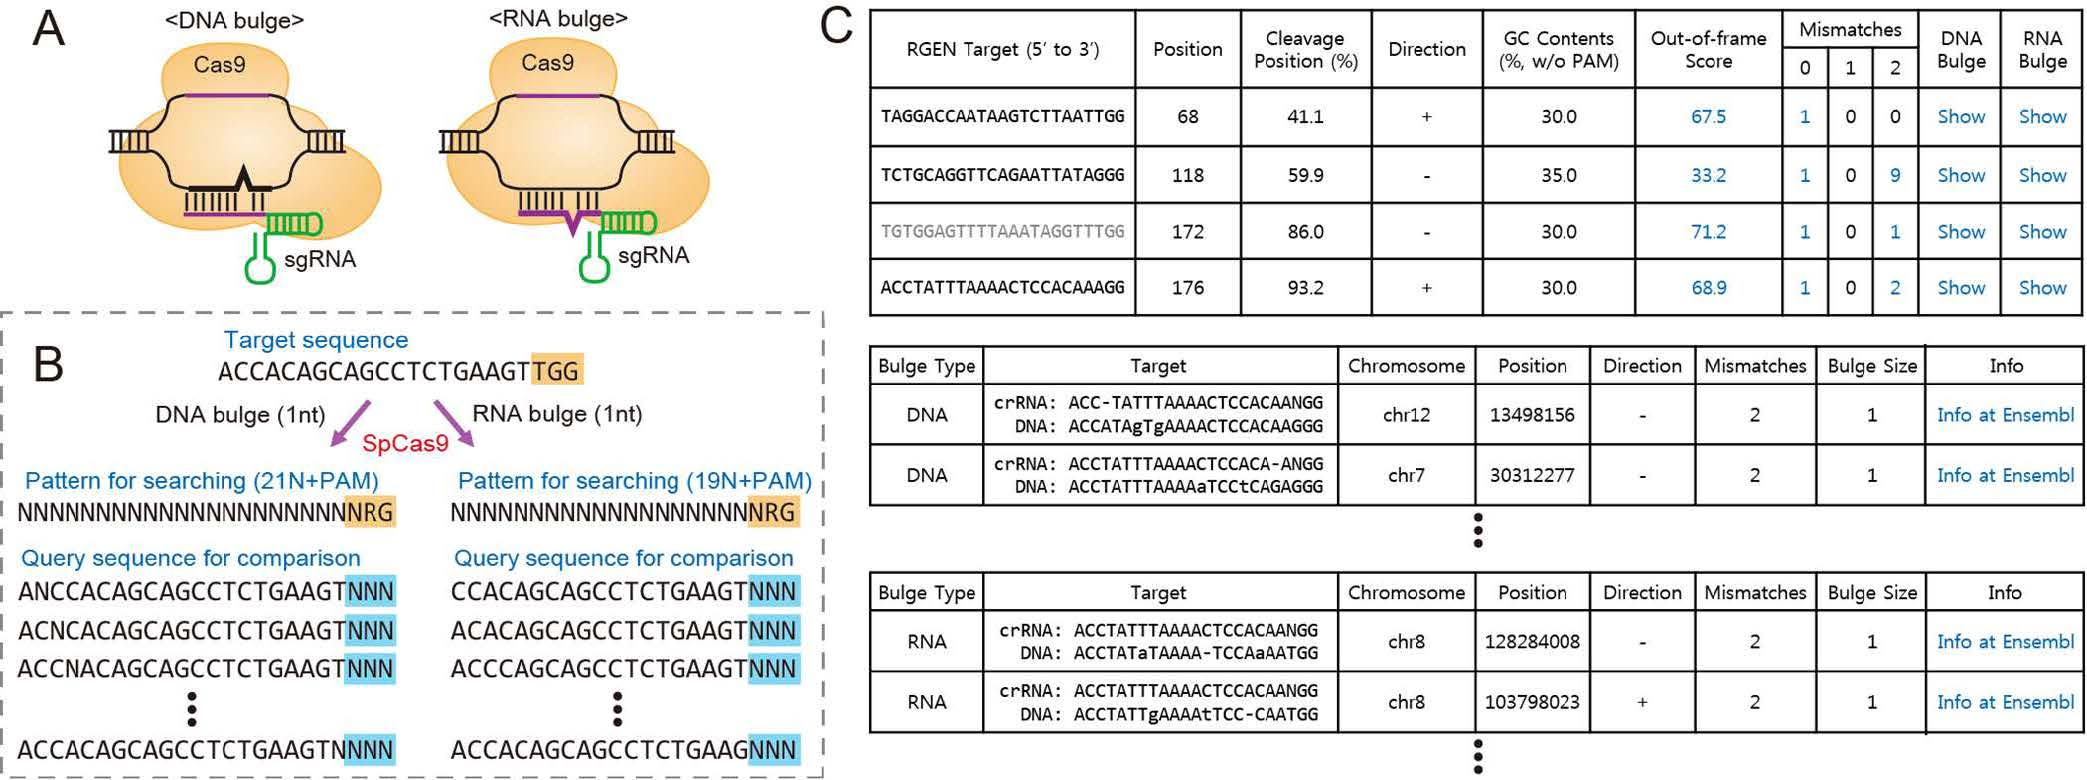
\includegraphics[width=16cm, ]{pictures/Cas-Designer.jpg}
\caption{
(الف) شماتیک مکان‌های off-tagets را با برآمدگی دی‌ان‌ای یا آر‌ان‌ای نشان می‌دهد. (ب) استراتژی برای  برآمدگی \lr{1-nt DNA} یا آر‌ان‌ای بر اساس Cas-OFFinder. ج) یک مثال
از یک جدول خروجی Cas-Designer تمام gRNA های ممکن را از توالی های ورودی به همراه اطلاعات مفید (بالا) نشان می دهد. اگر کاربر روی رنگ آبی کلیک کند
عدد، کلمه یا عبارت، اطلاعات دقیق تری مانند اهداف برآمدگی دی‌ان‌ای (وسط) یا آر‌ان‌ای (پایین) ارائه می شود. علاوه بر این، کاربر می تواند موارد مربوطه را به دست آورد
اطلاعات ژنومی از طریق مرورگر ژنوم Ensembl \lr{Flicek)} و همکاران، 2011)، با کلیک بر روی دکمه "اطلاعات در \lr{``Ensembl} \cite{Cas-OFFinder}
}\label{fig:4}
\end{figure}

ابتدا Cas-Designer سایت های طرح‌های احتمالی را با یک کاربر تعریف شده [\lr{50-NGG-30} یا \lr{50-NRG-30} برای \lr{SpCas9}, \lr{50-NNAGAAW-30} برای \lr{StCas9 (Cong et al., 2013)}, \lr{50-NNNNGMTT-30} برای \lr{NmCas9 (Hou et al., 2013)} و \lr{50-NNGRRT-30} برای \lr{SaCas9 (Ran et al., 2015)}] در یک توالی دی‌ان‌ای معین  پیدا می کند. در مرحله بعدی، Cas-Designer
امتیاز خارج از قاب مرتبط با میکروهومولوژی را به سرعت محاسبه می کند که با فراوانی جهش های تغییر قاب همبستگی مثبت دارد \lr{(Bae et al., 2014b)}. محتوای GC و امتیازات خارج از کادر در این مرحله موقعیت های برش را نشان می دهد.

\lr{Cas-OFFinder}
 از دو هسته OpenCL مختلف تشکیل شده است
( هسته جست‌وجوگر و یک هسته مقایسه‌گر ) و با C++ نوشته است. ابتدا Cas-OFFinder فایل های داده توالی ژنوم را به صورت تک یا چندتایی در فرمت FASTA می‌خواند. سپس در هسته جستجو بارگذاری می شود که تمام سایت هایی را که شامل یک توالی PAM در کل ژنوم هستند، کامپایل می کند. برای جستجو و انتخاب سریع و مؤثر این سایت‌های خاص، هسته جستجوگر به‌طور مستقل روی هر واحد محاسباتی یک پردازنده اجرا می‌شود، یعنی همه فرآیندهای جستجو در واحدهای محاسباتی به طور همزمان انجام می‌شوند.


\subsection{E-CRISP ~\cite{E-CRISP}}
\begin{wrapfigure}{l}{8.5cm}
\centering
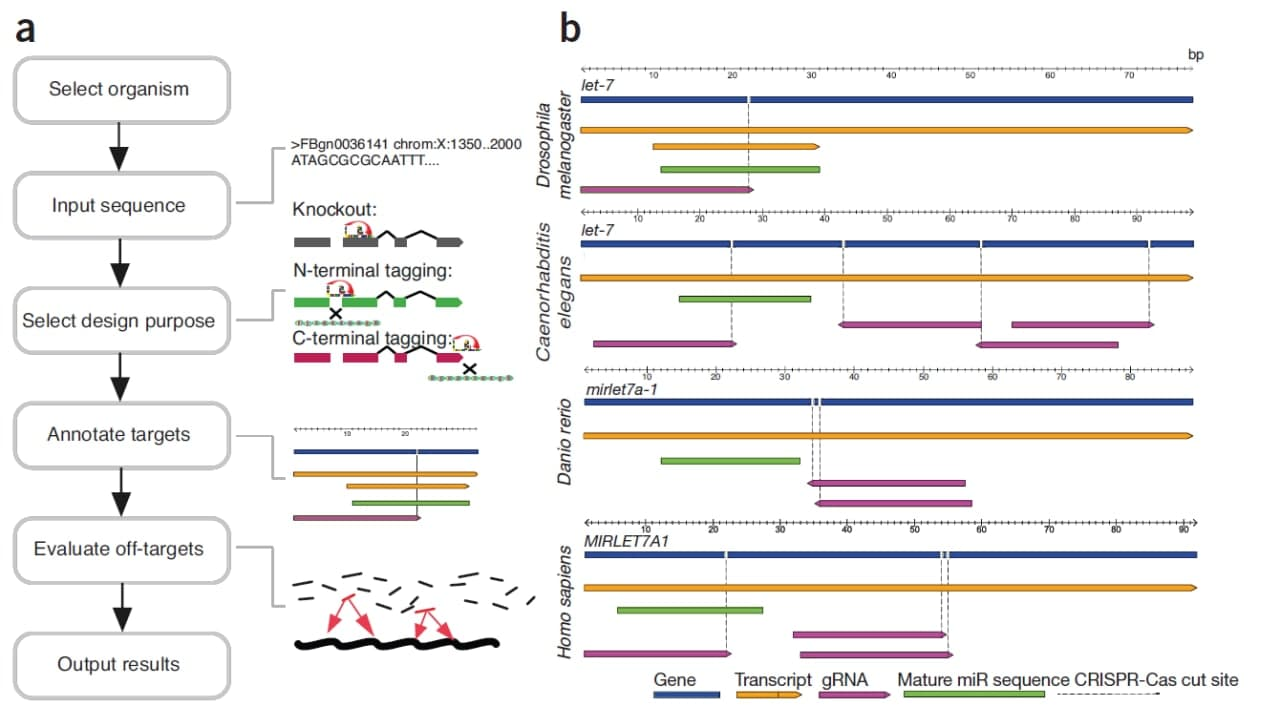
\includegraphics[width=10cm, ]{pictures/ecrispr.jpg}
\caption{
الگوریتم \lr{E-CRISP} \cite{E-CRISP}
}\label{wrap-fig:4}
\end{wrapfigure}

در اینجا ما E-CRISP، یک برنامه وب برای طراحی توالی های gRNA را توصیف می کنیم. (الف) مراحل E-CRISP. ابتدا کاربر ارگانیسم و دنباله هدف را انتخاب می کند. این هدف می تواند یک نماد ژن، یک شناسه ENSEMBL یا یک توالی FASTA باشد. در مرحله بعد، کاربر هدف آزمایش ویرایش را مشخص می کند. بسته به هدف، E-CRISP مناطق مختلفی از توالی ژن را مورد هدف قرار می دهد.
بعد از آن، E-CRISP نتایج را با توجه به اطلاعات حاشیه نویسی ژن فیلتر می کند. سپس، اهداف خارج از هدف بر اساس تراز توالی هر طرح با ژنوم مرجع تجزیه و تحلیل می شوند. در نهایت، E-CRISP یک صفحه خروجی تعریف شده توسط کاربر تولید می کند.
(ب) آر‌ان‌ای های راهنما در برابر جایگاه let-7 گونه های مشخص شده طراحی شده اند. توالی و محل gRNA های بالغ از miRBase بازیابی شده است. این خروجی انعطاف‌پذیر و پارامترهای طراحی آزمایش‌گرا را فراهم می‌کند، طراحی کتابخانه‌های متعدد و در نتیجه تجزیه و تحلیل سیستماتیک تأثیر پارامترهای مختلف را ممکن می‌سازد. E-CRISP توالی‌های هدف مکمل gRNA را شناسایی می‌کند که به یک موتیف که از سمت  '۳ مجاور به A)G یا N(G ختم می‌شود، که برای هسته Cas9 مورد نیاز است تا رشته دوگانه دی‌ان‌ای را برش دهد. E-CRISP از یک رویکرد نمایه سازی سریع برای یافتن مکان های اتصال و یک درخت فاصله دودویی برای حاشیه نویسی سریع سایت های هدف gRNA احتمالی استفاده می کند. با استفاده از این الگوریتم‌ها، می‌توان در چند ساعت کتابخانه‌هایی در مقیاس ژنومی برای چندین موجود زنده ایجاد کرد.
\subsection{CRISPOR~\cite{CRISPOR}}
\begin{wrapfigure}{l}{8cm}
\centering
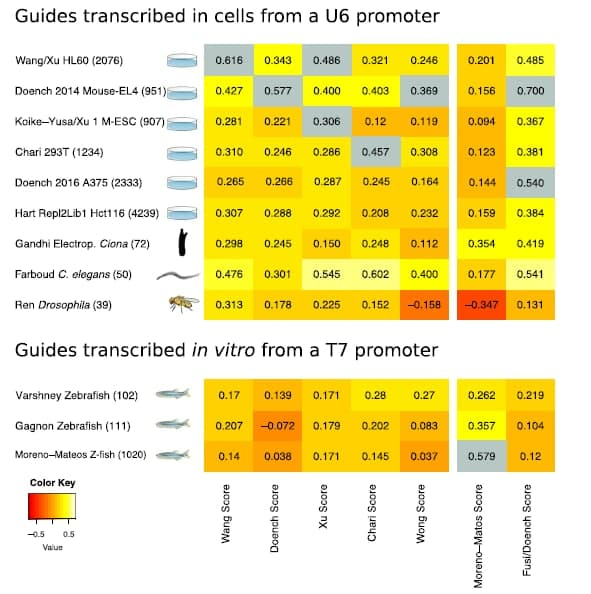
\includegraphics[width=9.5cm, ]{pictures/CRISPOR.jpg}
\caption{
هم بستگی اسپیرمن بین امتیاز موثر بودن و داده‌ها	\cite{CRISPOR}
}\label{wrap-fig:4}
\end{wrapfigure}
CRISPOR
 وب‌سایتی است که به انتخاب و بیان توالی‌های راهنمای CRISPR کمک می‌کند، که در دو مقاله توضیح داده شده است ( \lr {Gen Biol 2016} و \lr{NAR 2018} ). در حالت پیش فرض، کاربر یک توالی دی‌ان‌ای ورودی را چسبانده و ژنوم را انتخاب می کند. سپس CRISPOR راهنماها را در توالی ورودی فهرست می‌کند و اطلاعات مربوط به آنها را که در پایگاه‌های اطلاعاتی و الگوریتم‌ها یافت می‌شود، از جمله انواع ژنوم، امتیازهای پیش‌بینی‌شده off-targets و هدف، را اضافه می‌کند. برای هر دنباله راهنما، پرایمرهای مختلفی طراحی شده است، به عنوان مثال، برای تقویت هدف، آر‌ان‌ای های راهنما را با رونویسی آزمایشگاهی پس از بازپخت پرایمرهای همپوشانی یا برای شبیه سازی در پلاسمیدهای AddGene تولید می‌کند.
برای پیش‌بینی، داده‌ها را از هشت مطالعه \lr{،off-target} SpCas9 جمع‌آوری کردند و آنها را با سایت‌های پیش‌بینی‌شده توسط الگوریتم‌های محبوب مقایسه کردند و دریافتند که پیش‌بینی‌های off-target مبتنی بر توالی بسیار قابل اعتماد هستند، و اکثر اهداف خارج از هدف را با نرخ جهش بالاتر از \lr{ ۰.۱}٪ شناسایی می‌کنند، در حالی که تعداد موارد مثبت کاذب را می‌توان تا حد زیادی با یک برش، روی این امتیاز، حساسیت را افزایش داد. با توجه به آزمایشات مقاله به این دست یافتند که امتیاز موثر بودن به شدت به این بستگی دارد که آیا RNA راهنما از یک پروموتر U6 بیان می‌شود یا در شرایط آزمایشگاهی رونویسی می‌شود و با این ویژگی نشان دادند که می توان با زمان مناسب پیش‌بینی مناسبی ارائه داد.
\section{روش‌های یادگیری ژرف}
\subsection{پیش‌بینی off-target به کمک یادگیری ژرف}
\begin{wrapfigure}{l}{8cm}
\centering
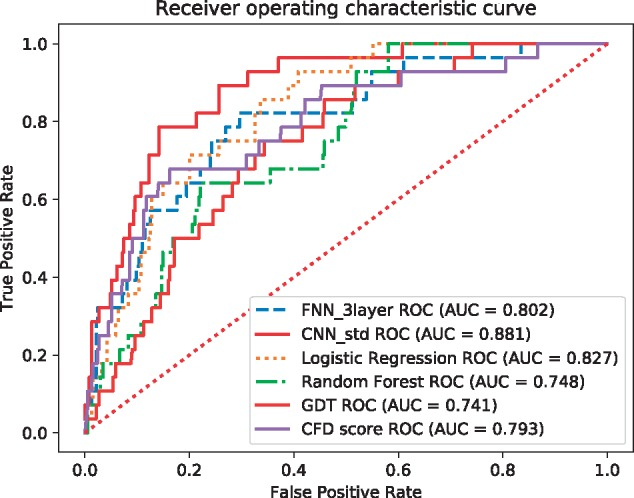
\includegraphics[width=9cm, ]{pictures/DeepLearning.jpg}
\caption{
هم بستگی اسپیرمن بین امتیاز موثر بودن و داده‌ها ~\cite{chart}
}\label{wrap-fig:4}
\end{wrapfigure}
پیش‌بینی جهش‌های خارج از هدف در CRISPR-Cas9 به دلیل ارتباط آن با تحقیقات ویرایش ژن یک موضوع پُر پژوهش‌ای است. روش های پیش بینی مختلفی توسعه یافته‌اند. با این حال، اکثر آنها فقط امتیازات را بر اساس عدم تطابق با دنباله راهنما در CRISPR-Cas9 محاسبه کردند. بنابراین، روش‌های پیش‌بینی موجود قادر به مقیاس‌بندی و بهبود عملکرد خود با گسترش سریع داده‌های تجربی در CRISPR-Cas9 نیستند. علاوه بر این، روش‌های موجود هنوز نمی‌توانند دقت کافی را در پیش‌بینی‌های خارج از هدف برای ویرایش ژن در سطح بالینی برآورده کنند. برای رفع این مشکل، در این پژوهش دو الگوریتم را با استفاده از شبکه‌های عصبی عمیق برای پیش‌بینی جهش‌های off-target در ویرایش ژن CRISPR-Cas9 طراحی و پیاده‌سازی می‌کنیم (با توجه به اطلاعات اولین الگوریتم ماشینی). این مدل‌ها بر روی مجموعه داده‌های اخیراً منتشر شده، مجموعه داده‌های CRISPOR، برای معیار عملکرد، آموزش دیده و آزمایش شدند. یکی دیگر از مجموعه داده شناسایی شده توسط GUIDE-seq برای ارزیابی بیشتر مورد استفاده قرار گرفت. مقاله نشان می‌دهد که شبکه عصبی کانولوشن بهترین عملکرد را در مجموعه داده‌های CRISPOR به دست می‌آورد، و سطح طبقه‌بندی متوسط ​​زیر منحنی ۹۷.۰ درصد را تحت اعتبارسنجی متقاطع 5 برابری طبقه‌بندی شده به دست می‌آورد. جالب اینجاست که شبکه عصبی پیشخور عمیق نیز می‌تواند با میانگین ۹۷.۰ در همان تنظیمات رقابتی باشد. ما دو مدل شبکه عصبی عمیق را با روش‌های پیشرفته پیش‌بینی off-target ( مانند CFD، MIT، CROP-IT، و CCTop ) و سه مدل سنتی یادگیری ماشین (یعنی جنگل تصادفی، درخت‌های تقویت‌کننده گرادیان، و رگرسیون لجستیک) در هر دو مجموعه داده از نظر مقادیر AUC، نشان دهنده لبه های رقابتی الگوریتم های پیشنهادی است. تحلیل های اضافی برای بررسی دلایل زمینه ای از دیدگاه های مختلف انجام می شود.

\subsection{CCTop~\cite{CCTop}}
این روش طرح‌های مختلفی که به صورت N20NGG هستند را دسته بندی کند، ابتدا با آزمایش‌های عملی طرح‌ها را به دو کلاس موٍثر و ناموثر دسته‌بندی کرده‌اند. آزمایش به این گونه بود که طرح را  در محیط آزمایشگاهی به ژن تزریق می کردند و برای هر طرح، تعداد هدف‌های تغییر کرده در طول زمان یادداشت کرده‌اند. این روش بر این باور بود که ribosomal و non-ribosmal بودن ژن در تاثیر طرح موثر است پس دیتاست خود را به دو قسمت تقسیم کرده و برای طرح هر کدام sgrna موثر و ناموثر را تعیین کرده است. این طرح جایگاه هر نیکلوتید را در sgrna های موثر و ناموثر برسی کرده و به نتایج زیر رسیده است.\\
نحوی انتخاب موثر یا ناموثر بودن یک طرح با کمک مدل حسب مدل  Elastic-Net است که در آن اگر
 $X_i$
encode شده طرح ها باشند
و Yها امتیاز آن‌ها باشد داریم:
\\
پس از آموزش این مدل، به کمک آزمایش‌های آماری به ۲۸ ویژگی مختلف تاثیرگذاری رسیدند که بیشتر این ویژگی‌ها در ناحیه اسپیسر واقع شده‌اند و بعضی از آنها قبلا پیدا شده بود و بعضی جدید بود، که چند نمونه از این دست یافت‌های جدید عبارت اند از:
\begin{itemize}
\item
 قرار گرفتن نیکلوتید G در موقعیت های ۱- و ۲- نسبت به PAM در CAS9 باعث افزایش تاثیرگذاری می‌شود.
\item 
قرار گرفتن نیکلوتید T در چهار موقعیت نزدیک به PAM باعث کاهش تاثیرگذاری می‌شود.
\item
  نوکلئوتیدهای رشته '۵ به '۳ تاثیرگذار هستند، در حالی که رشته مکمل تاثیر قابل توجهی ندارد.
\item
قرار گرفتن نیکلوتید C در موقعیت ۳- در CAS9 باعث افزایش تاثیرگذاری می‌شود.
\item
 
قرار گرفتن نیکلوتید A در موقعیت -5 تا -12 باعث افزایش تاثیرگذاری می‌شود.
\item 
قرار گرفتن نیکلوتید G در موقعیت های -14 تا -17 باعث افزایش تاثیرگذاری می‌شود.
\end{itemize}

\section{DeepCRISPR}
DeepCRISPR ، 
یک پلتفرم محاسباتی جامع برای یکپارچه سازی پیش‌بینی ناحیه‌ sgRNA روی هدف و خارج از هدف در یک چارچوب با یادگیری عمیق، با استفاده از پیشرفته‌ترین ابزارهای موجود در سیلیکون است. DeepCrispr \cite{DeepCRISPR} علاوه بر ویژگی های توالی دی‌ان‌ای، چهار ویژگی اپی ژنتیکی را معرفی کرد و به طور خودکار اطلاعات معتبر را با استفاده از اصل Auto-encoder استخراج می کند. چندین مدل از جمله برش هدف sgRNA و پیش‌بینی تمایل خارج از هدف ایجاد شد. پژوهشگران بر این باور بودند که خود دنباله sgRNA می‌تواند اطلاعات مفید درباره موثر بودن یک توالی sgRNA بدهد به همین امر مدل خود را به دو گونه آموزش دادن با در نظر گرفتن اطلاعات اپی ژنتیکی و بدون دانستن اطلاعات اپی ژنتیکی که نشان می‌دهد که اطلاعات اپی ژنتیکی بی تاثیر نیست. 
\begin{figure}[H]
\centering
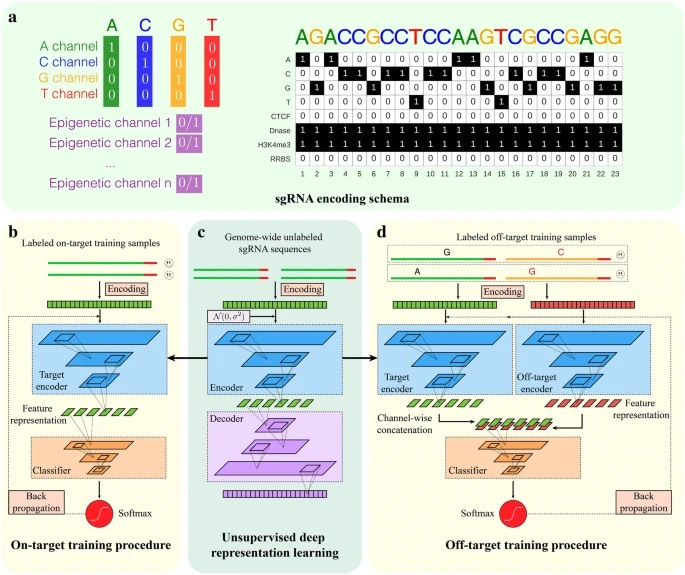
\includegraphics[width=10cm, ]{pictures/DeepCRISPR.jpg}
\caption{
DeepCRISPR~\cite{DeepCRISPR}
}\label{wrap-fig:4}
\end{figure}

\begin{table}[H]
    \caption{خلاصه‌ای از کار‌های پیشین}
\begin{adjustbox}{center}
\resizebox{1.1\columnwidth}{!}{%
    \begin{tabularx}{1.1\textwidth}{|Y|Y|Y|Y|Y|Y|Y|}
    	\rowcolor{Goldenrod}	

	\lr{Features}& \lr{Off-Target Scoring Method} & \lr{On-Target Scoring Method} & \lr{Organism} & \lr{Enzyme} & \lr{Input} & \lr{Method} \\ \hline

	\lr{\scriptsize
{Designs primers for the edited site amplification; restriction sites map; exon-intron map;
Integrates Shen et al. 2018 predictions of repair profile}}& \lr{MIT specificity score;
Cong et al., 2013} & \lr{{\scriptsize Doench et al. 2014;
Doench et al. 2016;
Chari et al. 2015;
Xu et al. 2015;
Moreno-Mateos et al. 2015;
G20}} & \lr{Variety} & \lr{SpCas9; SpCas9n; Cas12a (Cpf1); CasX; Cas13 (C2C2);
TALEN} & \lr{GeneID
Coordinates
Sequence} & \lr{CHOPCHOP} \\ \hline

	\lr{\scriptsize
{Designs primers for the edited site amplification; restriction sites map; provides sequences for in vitro expression or cloning of designed sgRNAs;
Integrates Bae et al. 2014 predictions of repair profile and Chen et al. 2018 frameshift prediction}}& \lr{MIT Specificity Score;
CFD Specificity score} & \lr{Doench et al. 2016
Chari et al. 2015;
Xu et al. 2015;
Wu-Crisp
Doench et al. 2014;
Wang et al. 2014
Moreno-Mateos et al. 2015;
Azimuth in-vitro
crisprRank} & \lr{Variety} & \lr{{\scriptsize SpCas9; SpCas9-HF1; eSpCas9 1.1;
ScCas9;
iSpyMacCas9; SaCas9; xCas9;
SaCas9-KKH;
SpCas9-VQR;
NmeCas9;
SpCas9-VRER;
StCas9; CjCas9; AsCas12a (Cpf1);
LbCas12a (Cpf1)}} & \lr{Coordinates
Sequence} & \lr{CRISPOR} \\ \hline

	\lr{Includes genetic variation}& \lr{Bowtie2} & \lr{Heighwer et al. 2014;
Doench et al. 2014;
Xu et al. 2015} & \lr{Variety} & \lr{SpCas9} & \lr{GeneID
Sequence} & \lr{E-CRISP} \\ \hline

	\lr{Features}& \lr{Exome-wide catalog of Cas9 cleavage sites} & \lr{Aach et al. 2014} & \lr{Homo sapiens
Mus musculus} & \lr{SpCas9; StCas9; NmeCas9} & \lr{Coordinate
Sequence} & \lr{CasFinder CasDesigner} \\ \hline
	\lr{Includes genetic variation}& \lr{Stemmer et al.
2017} & \lr{CRISPRater} & \lr{Variety} & \lr{{\scriptsize
SpCas9; SpCas9-VQR;
SpCas9-VRER; AsCas12a (Cpf1);
LbCas12a (Cpf1);
FnCas12a (Cpf1);
SaCas9; StCas9; NmeCas9; TdCas9}} & \lr{Sequence} & \lr{CCTop} \\ \hline

	\lr{Integrates the epigenetic information in different cell types}& \lr{Chuai et al. 2018} & \lr{Chuai et al. 2018} & \lr{Homo sapiens} & \lr{SpCas9} & \lr{Sequence} & \lr{DeepCRISPR} \\ \hline

    \end{tabularx}}
\end{adjustbox}
\end{table}

با توجه به این که کار‌های پیشین روی اورگان‌های مختلف آموزش داده شده بودند در اورگان‌هایی که تا به حال ندیده اند، نتایج خوبی ندارند و همین‌طور با اینکه دقت این مدل‌ها بالا است، هنوز به دقتی قابل اعتماد تبدیل نشده‌اند، در نتیجه در این پژوهش ما سعی می‌کنیم که برای این مشکلات راه حلی بهتری ارائه دهیم.

\chapter{روش‌های پیشنهادی}
ابتدا یک بار دیگه مسئله را مدل سازی می‌کنیم، فرض کنید یک رشته ۲۳ تایی از نوکلوتید‌ها را در اختیار داریم، پس اگر $N$ ، یک نوکلوتید دلخواه باشد، رشته دلخواه به صورت زیر است:
$$
NNNNNNNNNNNNNNNNNNNNNNN
$$
از آنجایی که در پژوهش ما فقط از cas9 استفاده می‌شود دو نوکلوتید آخر باید G باشد پس داریم:
$$
NNNNNNNNNNNNNNNNNNNNNGG
$$
به این رشته ۲۳تایی، ترکیب ۲۰‌تایی sgRNA و ۳تایی PAM می گویند که برای cas9 ، حتما باید NGG باشد. 
تمام کارهای پیشین به روشی این رشته ۲۳تایی را با توجه به ویژگی‌های مختلف یا اینکدینگ به متغیر کمی تبدیل کرده‌اند. پس به عنوان ورودی این رشته و ویژگی‌های مختلف را استفاده می‌کنند تا به عنوان خروجی یک عدد بین صفر و یک به عنوان امتیاز تاثیرگذاری به ما می دهند. داده‌های امتیاز تاثیرگذاری به صورت آزمایشگاهی توسط پژوهشگران با ادغام طرح کریسپر با سلول هدف و یادداشت نتایج آن در طول زمان بدست می‌آید. این نتایج با توجه به پژوهش متفاوت می باشد که یک مشکل برای ادغام داده‌ها می باشد از جلمه دو مورد از نتایج نظارت شده هنگام این آزمایش‌ها، شمردن ایندل‌ها و شمردن تعداد شکست‌های دی‌ان‌ای است. همچنین شایان ذکر است که تاثیرگذاری sgRNA ها در جانور‌های مختلف و اورگان‌های مختلف متفاوت است ولی با توجه به پژوهش‌های صورت گرفته مانند DeepCRISPR \cite{DeepCRISPR} هم چنان با نادیده گرفتن این اطلاعات و تمرکز روی رشته sgRNA نیز می‌توان پیش‌بینی‌های مفیدی انجام داد. با در نظر گرفتن این فرضیات نیز هنوز فضای مسئله فضای بسیار بزرگی است از آنجا که تعداد طرح‌های ممکنه با تعداد جایگشت، با تکرار ۴ شی در ۲۱ خانه یا همان 
$4^{21} \approx 4.3980465 \times 10^{12}$
است. در نتیجه با دیدن حدود ۱۰ هزار یا حتی ۱۰۰ هزار نمونه نمی‌توان نتیجه‌ی عمومی درباره‌ی این مسئله گرفت.
برای درست کردن روشی عمومی، به داده‌های زیاد و دقیق نیاز است که در حال حاضر در دسترس نیستند و همین‌طور معمولا این دادگان برای یک روش خاص تهیه شده‌اند که یعنی بعضی از ویژگی‌های مورد نیاز برای بعضی داده‌ها موجود و برای برخی دیگر موجود نیستند، از آنجا که قادر به درست کردن مجموعه داده مناسب و عمومی نبوده‌ایم، سعی کردیم با کمترین ویژگی‌ها مدلی بسازیم که بهترین دقت را داشته باشد، یعنی فقط دنباله دی‌ان‌ای. در این پژوهش، ما دو ایده برای تبدیل متغیر کیفی sgRNA به متغیر کمی داشتیم. ایده اول استفاده از نتایج کار‌های پیشین به عنوان نمایش بردار کمی sgRNA بود و ایده دوم استفاده از مدل‌های attention و transformer ها برای بدست آوردن یک کدگذاری مناسب است.

 از آنجا که بیشتر کار‌های پیشین ویژگی‌های دیگر مورد نیاز خود را از ورودی متد‌ها نمی‌گرفتند یک روش مناسب برای حذف این ویژگی‌های اضافه و کمک به عمومی شدن مدل، ادغام متد‌های مختلف است ولی با توجه به نتایج ادغام، این مدل‌ها به تنهایی کافی نیست، در نتیجه برای رفع این مشکل، ما از روشی نوین که ایده‌ای مشابه به \lr{Stacked Generalization}  \cite{Stacking} دارد استفاده می‌کنیم تا با مجموعه دادگان کم، دقت بهتری بدست‌آوریم. می‌توان به روش بدست آمده مانند اصلاح اشتباهات یک مدل توسط مدل دیگر نگاه کرد که در آن از چند مدل مختلف چندین نمونه داریم که همگی باهم ادغام می‌شوند تا بهتر نتیجه از یک مدل بدست بیاید و برای بدست آمدن بهترین نتیجه هر مدل برای این که متر مناسب و معلومی وجود ندارد چندین یک از پر کاربردترین خطا‌ها را استفاده کردیم و مدل را با آن فاینتون کردیم و با رائ‌گیری بین همه خطا‌های مختلف نتیجه‌ی پیشبینی مدل را به عنوان بهترین جواب مدل در نظر گرفتیم. با بدست آمدن بهترین نمونه از هر مدل، مدل‌ها را با هم ادغام می کنیم تا با اصلاح یک دیگر بهترین دقت را به ما ارائه دهند. واضح است که ممکن است دو مدل مختلف نقاط ضعف و قوت مشترکی داشته باشند که در این صورت روش ذکر شده مفید نخواهد بود.
\section{Ensemble Learning}
در آمار و یادگیری ماشین، روش‌های ensemble از الگوریتم‌های یادگیری چندگانه استفاده می‌کنند تا عملکرد پیش‌بینی‌کننده بهتری نسبت به هر یک از الگوریتم‌های یادگیری سازنده به‌تنهایی به‌دست آورند. ~\cite{Opitz, Polikar, Rokach} بر خلاف ensemble آماری، که معمولاً از بی نهایت مکانیک آماری استفاده می‌کند، یک مجموعه یادگیری ماشینی تنها از مجموعه محدود مشخصی از مدل‌های تشکیل شده است، اما معمولاً ساختار بسیار انعطاف‌پذیرتری را در بین آن گزینه‌ها امکان می‌دهد.
\subsection{تعریف}
الگوریتم های یادگیری نظارت شده وظیفه جستجو در فضای فرضیه را برای یافتن یک فرضیه مناسب انجام می دهند که پیش بینی های خوبی را با یک مسئله خاص انجام دهد.~\cite{Blockeel}

ارزیابی پیش‌بینی یک مجموعه معمولاً به محاسبات بیشتری نسبت به ارزیابی پیش‌بینی یک مدل نیاز دارد. از یک جهت، یادگیری گروهی ممکن است به عنوان راهی برای جبران الگوریتم های یادگیری ضعیف با انجام محاسبات زیاد در نظر گرفته شود. از سوی دیگر، جایگزین این است که یادگیری بسیار بیشتری را در یک سیستم غیر گروهی انجام دهید. یک سیستم ensemble ممکن است در بهبود دقت کلی برای افزایش یکسان در منابع محاسباتی، ذخیره‌سازی یا ارتباطی با استفاده از این افزایش در دو یا چند روش، کارآمدتر از افزایش استفاده از منابع برای یک روش واحد باشد. الگوریتم‌های سریع مانند درخت‌های تصمیم معمولاً در روش‌های ensemble (مثلاً جنگل‌های تصادفی) استفاده می‌شوند، اگرچه الگوریتم‌های کندتر می‌توانند از تکنیک‌های مجموعه نیز بهره ببرند.

برای اینکه بتوان از این روش‌ استفاده کرد نیاز است که ابتدا جواب این مدل‌ها یا اکسپرت‌ها را روی یک دیتای مشابه داشته باشیم، مقاله‌ی DeepCRISPR دقیقا داده ۴۲۵ دنباله sgRNA از امتیاز دهنده‌های ۵ مقاله و امتیاز مقاله خود تهیه کرده که از آنها استفاده کردیم. چندین روش ensemble برای جمع این امتیاز‌ها و رتبه بندی‌ها استفاده کردیم، مانند وزن دهی بر حسب دقت هر مدل روی یک دیتا ثابت و همین طور روش‌ LPA یا \lr{Latent Profie Analysis} که به ما مدلی برحسب پیشبینی مدل‌هایی دیگر می دهند. از این روش‌ها ما دو مدل بدست آوردیم ولی دقت این مدل‌ها همگی از مدل DeepCRISPR پایین تر بودند با آنالیز بیشتر به این نتیجه رسیدیم که این مدل‌ها بر سر بعضی نقاط شدیدا اختلاف نظر دارند که باعث تاثیر منفی در نتیجه ensemble این مدل‌ها می‌شود و با این گونه وزن دهی نمی‌توان به نتیجه بهتری رسید. در بخش نتایج، نمونه‌هایی از این روش‌ها را نشان می‌دهیم.

در مرحله بعدی با جنگل‌های تصادفی سعی کردیم فضای مسئله را تقسیم کنیم و بر اساس آن از امتیاز مدل‌های دیگر استفاده کنیم تا بتوانیم جواب بهتری بدست آوریم، پس از تنظیم کردن ابرپارامترها توانستیم به مدلی بهتر از مدل‌های قبلی برسیم ولی با انجام cross-validation به این نتیجه رسیدیم که دیتای استفاده شده برای آموزش تاثیر زیادی روی دقت پیشبینی دارد و لزوما این روش همیشه از روش DeepCRISPR بهتر نیست، برای بدست آوردن مدل قوی نیاز به دیتای بیشتر داشتیم.

در مرحله‌ی آخر، با توجه به اینکه اکسپرت‌ها اختلاف نظر داشتند و ensemble کردن این اکسپرت‌ها اختلاف نظر آنها را کم می کرد،‌ چهار الگوریتم، رگرسیون با جنگل تصادفی \lr{(Random Forest)}، درختان بسیار تصادفی \lr{(Extra Trees)}، حداقل مربعات معمولی \lr{(Ordinary Least Squares)}، تقویت گرادیان \lr{(Gradient Boosting)} را برای ensemble اکسپرت‌ها انتخاب کردیم. هر کدام از الگوریتم‌ها به تنهایی به داده آموزش حساس بودند و با انجام cross-validation لزوما به نتیجه بهتری نمی رسیدند ولی برخلاف اکسپرت‌‌های اولیه اختلاف نظر این رگرسورها خیلی کم بود پس این متد‌ها را با هم ادغام کردیم و به نتیجه‌ی مطلوب رسیدیم، یعنی مدلی آموزش داده شده به نویز داده آموزش حساس نبود و با هر فولدی باز‌ هم از روش DeepCRISPR بهتر عمل می‌کرد.

برای اینکه مشکل داده کم را حل کنیم، ما ابتدا ۲۷۰۵ توالی مختلف را در الگوریتم‌های
 Cas-Designer ، CCTop ، E-Crisp ، CRISPOR و Chopchop جمع آوری کردیم، که منجر بدست آمدن ۵۰هزار sgRNA یکتا شد و از آنجا که خروجی الگوریتم‌ها می توانست NaN هم باشد، با حذف این داده‌ها به ۳۶هزار sgRNA یکتا و نظر اکسپرت‌ها راجع به آن رسیدیم. تنها کافی بود که بتوانیم یک golden standard برای این داده‌ها پیدا کنیم، که متاسفانه قادر به این کار نشدیم. 
\subsection{رگرسیون با جنگل تصادفی}
رگرسیون با جنگل تصادفی \cite{Random Forests} یک الگوریتم یادگیری نظارت شده است که از روش یادگیری ادغامی برای رگرسیون استفاده می کند.
\subsubsection{مقدمات: آموزش درخت تصمیم}
درخت تصمیم روش مشهوری برای انواع مختلفی از وظایف یادگیری ماشین به حساب می آید. با این حال در بسیاری موارد دقیق نیستند.

در کل، معمولا درخت تصمیمی که بیش از حد عمیق باشد الگوی دقیقی نخواهد داشت: دچار بیش‌برازش شده، و دارای سوگیری پایین و واریانس بالا می‌باشد. جنگل تصادفی روشی است برای میانگین گیری با هدف کاهش واریانس با استفاده از درخت‌های تصمیم عمیقی که از قسمت‌های مختلف داده آموزشی ایجاد شده باشند. در این روش معمولا افزایش جزئی سوگیری و از دست رفتن کمی از قابلیت تفسیر اتفاق افتاده اما در کل عملکرد مدل را بسیار افزایش خواهد داد.
\subsubsection{کیسه‌گذاری درختان}
مجموعه داده را با ${\displaystyle D}$ نمایش میدهیم، ${\displaystyle D=(x_{1},y_{1}),(x_{2},y_{2}),\cdots ,(x_{n},y_{n})}$ و ${\displaystyle B}$ درخت تصادفی با ایجاد ${\displaystyle B}$ داده جدید از ${\displaystyle D}$ ایجاد می‌کنیم. مدل نهایی با میانگین گرفتن یا رأی‌گیری بین درختان کار می‌کند. جزئیات این الگوریتم ذیلاً آمده است:‌

برای ${\displaystyle B}$ تا ${\displaystyle b=1}$:

\begin{itemize}
\item ${\displaystyle n}$
 نمونه با جایگزینی از داده ${\displaystyle D}$ انتخاب می‌کنیم و این نمونه‌ها را در مجموعه داده ${\displaystyle D_{b}}$ قرار می‌دهیم. از آنجا که نمونه‌گیری با جایگزینی صورت می‌گیرد یک نمونه ممکن است چندین بار انتخاب شود.
\item
 یک درخت تصادفی به اسم ${\displaystyle T_{b}}$ با ${\displaystyle D_{b}}$ به روش پایین می‌سازیم:\\
 هر دفعه برای پیدا کردن بهترین متغیر ابتدا یک تعداد مشخصی از متغیرها را کاملا به صورت تصادفی انتخاب می‌کنیم (مثلا ${\displaystyle m}$ متغیر اول به مسئله داده شده‌است، و معمولاً با جذر تعداد متغیرها برابر است) و از میان آن‌ها بهترین متغیر را انتخاب می‌کنیم.
\end{itemize}
در مسئله رگرسیون مدل نهائی، میانگین تمامی درخت‌ها است یعنی ${\displaystyle F(x)={\frac {1}{B}}\sum _{b=1}^{B}T_{b}(x)}$. از طرفی دیگر در مسئله دسته‌بندی با رأی‌گیری بین درختان به جواب نهائی می‌رسیم.

این نوع ترکیب مدل‌ها جواب بهتری به ما می‌دهد، زیرا گوناگونی و تنوع مدل‌ها را افزایش می‌دهد، بدون این که بایاس را افزایش دهد. این بدین معناست، زمانی که پیش‌بینی تکی از یک درخت دارای نویز بالایی درون مجموعه دسته آموزش دیده‌اش باشد، در میانگین بسیاری از درخت‌ها این نویز وجود نخواهد داشت. به شکل ساده آموزش درختان به صورت تکی می‌تواند درخت‌های در ارتباط قوی تری را ارائه دهد. بوت استرپ کردن نمونه، روشی برای یکپارچه‌تر کردن درخت‌ها با نمایش مجموعه داده‌های آموزش دیده گوناگون است.

\begin{figure}[H]
\centering
\scalebox{0.5}{
\begin{forest}
  for tree={l sep=3em, s sep=3em, anchor=center, inner sep=0.7em, fill=blue!50, circle, where level=2{no edge}{}}
  [
  Training Data, node box
  [Sample and Feature Bagging, node box, alias=bagging, above=4em
  [,red!70,alias=a1[[,alias=a2][]][,red!70,edge label={node[above=1ex,red arrow]{}}[[][]][,red!70,edge label={node[above=1ex,red arrow]{}}[,red!70,edge label={node[below=1ex,red arrow]{}}][,alias=a3]]]]
  [,red!70,alias=b1[,red!70,edge label={node[below=1ex,red arrow]{}}[[,alias=b2][]][,red!70,edge label={node[above=1ex,red arrow]{}}]][[][[][,alias=b3]]]]
  [~~$\dots$~,scale=2,no edge,fill=none,yshift=-4em]
  [,red!70,alias=c1[[,alias=c2][]][,red!70,edge label={node[above=1ex,red arrow]{}}[,red!70,edge label={node[above=1ex,red arrow]{}}[,alias=c3][,red!70,edge label={node[above=1ex,red arrow]{}}]][,alias=c4]]]]
  ]
  \node[tree box, fit=(a1)(a2)(a3)](t1){};
  \node[tree box, fit=(b1)(b2)(b3)](t2){};
  \node[tree box, fit=(c1)(c2)(c3)(c4)](tn){};
  \node[below right=0.5em, inner sep=0pt] at (t1.north west) {Tree 1};
  \node[below right=0.5em, inner sep=0pt] at (t2.north west) {Tree 2};
  \node[below right=0.5em, inner sep=0pt] at (tn.north west) {Tree $n$};
  \path (t1.south west)--(tn.south east) node[midway,below=4em, node box] (mean) {Mean in Regression or Majority Vote in Classification};
  \node[below=3em of mean, node box] (pred) {Prediction};
  \draw[black arrow={5mm}{4mm}] (bagging) -- (t1.north);
  \draw[black arrow] (bagging) -- (t2.north);
  \draw[black arrow={5mm}{4mm}] (bagging) -- (tn.north);
  \draw[black arrow={5mm}{5mm}] (t1.south) -- (mean);
  \draw[black arrow] (t2.south) -- (mean);
  \draw[black arrow={5mm}{5mm}] (tn.south) -- (mean);
  \draw[black arrow] (mean) -- (pred);
\end{forest}}
\end{figure}
\subsection{درختان بسیار تصادفی}
در درختان بسیار تصادفی\cite{Extremely randomized trees}، یک قدم تصادفی بیشتر دارد. همانند جنگل‌های تصادفی، زیرمجموعه‌ای تصادفی از متغیرها کاندید می‌شود، اما به جای جستجوی بهترین آستانه، آستانه‌ها به‌طور تصادفی برای هر متغیر کاندید شده ترسیم می‌شود و بهترین این آستانه‌های تصادفی تولید شده به عنوان آستانه تقسیم انتخاب می‌شوند. این امر عموما به کاهش کمی بیشتر واریانس مدل منجر می‌شود و باعث افزایش کوچکی در بایاس می‌شود.
\subsection{حداقل مربعات معمولی}
در آمار، حداقل مربعات معمولی (به انگلیسی: \lr{Ordinary Least Squares}) (به اختصار OLS )، روشی است برای برآورد پارامترهای مجهول در مدل رگرسیون خطی از طریق کمینه کردن اختلاف بین متغیرهای جواب مشاهده شده در مجموعه داده است. فرض کنید که $n$ مشاهده‌ی
 $\left\{\mathbf {x} _{i},y_{i}\right\}_{i=1}^{n}$
 داریم.
هر مشاهده $i$ شامل یک پاسخ اسکالر $y_{i}$ و یک بردار ستونی $\mathbf {x}_{i}$ از پارامترهای $p$ (رگرسور) ، به عنوان مثال، 
$\mathbf {x}_{i}=\left[x_{i1},x_{i2},\dots ,x_{ip}\right]^{\mathsf { T}}$
. در یک مدل رگرسیون خطی، متغیر پاسخ، $y_{i}$، یک تابع خطی از رگرسورها است:
$${\displaystyle y_{i}=\beta _{1}\ x_{i1}+\beta _{2}\ x_{i2}+\cdots +\beta _{p}\ x_{ip}+\varepsilon _{i},}$$
که از به عنوان بردار به آن نگاه کنیم داریم:
$$
{\displaystyle y_{i}=\mathbf {x} _{i}^{\mathsf {T}}{\boldsymbol {\beta }}+\varepsilon _{i},\,}
$$
به طوری که ${\displaystyle}\mathbf {x} _{i}$ بردار ستونی از
 ${\displaystyle i}$-امین مشاهده همه متغیرهای است و
 ${\displaystyle\boldsymbol {\beta}}$	
 یک بردار ${\displaystyle p\times 1}$ از پارامترهای ناشناخته است. و اسکالار
 ${\displaystyle \varepsilon _{i}}$
 نشان دهنده متغیرهای تصادفی مشاهده نشده (خطاهای) مشاهده 
${\displaystyle i}$-ام است.
${\displaystyle \varepsilon _{i}}$
 تأثیرات توضیح‌دهنده‌های
 ${\displaystyle y_{i}}$ 
توسط
${\displaystyle \mathbf {x} _ {i}}$
نشان می‌دهد.
 این مدل را می توان به صورت نماد ماتریسی نیز نوشت:
$$
{\displaystyle \mathbf {y} =\mathrm {X} {\boldsymbol {\beta }}+{\boldsymbol {\varepsilon }},\,}
$$

به طوری که ${\displaystyle \mathbf {y} }$ و ${\displaystyle {\boldsymbol {\varepsilon}}}$ بردارهای
 ${\displaystyle n\times 1}$ هستند متغیرهای پاسخ و خطاهای ${\displaystyle n}$ مشاهدات و ${\displaystyle \mathrm {X} }$ یک ماتریس ${\displaystyle n\times p}$ از رگرسیون‌ها است. گاهی اوقات ماتریس طراحی نیز نامیده می شود که سطر ${\displaystyle i}$-ام آن $ {\displaystyle \mathbf {x} _{i}^{\mathsf {T}}}$ است و حاوی مشاهدات ${\displaystyle i}$-ام روی همه متغیرهای توضیحی است.

رگرسورها لازم نیست مستقل باشند: هر رابطه دلخواه بین رگرسیون ها می تواند وجود داشته باشد (تا زمانی که یک رابطه خطی نباشد). برای مثال، ممکن است مشکوک باشیم که پاسخ به صورت خطی هم به مقدار و هم به مربع آن بستگی دارد. در این صورت یک رگرسیون را که مقدار آن فقط مجذور رگرسیور دیگر است را در نظر می گیریم. در آن صورت، مدل در رگرسور دوم، درجه دوم خواهد بود، اما با این حال، همچنان یک مدل خطی در نظر گرفته می‌شود، زیرا مدل همچنان در پارامترهای خطی است.

از آنجایی که $\varepsilon _{i}$ قابل محاسبه نیست برای استفاده از این روش معادله زیر را درنظر بگیرید:
$$
{\displaystyle \sum _{j=1}^{p}X_{ij}\beta _{j}=y_{i},\ (i=1,2,\dots ,n),\ n>p}
$$
چنین دستگاهی معمولاً راه حلی برای رسیدن به جواب دقیق ندارد، بنابراین هدف یافتن ضرایب ${\displaystyle {\boldsymbol {\beta }}}$ است که نزدیکترین حالت به جواب می باشد، به معنای دیگر حل مسئله کمینه سازی درجه دوم ${\hat {\boldsymbol {\beta }}}={\underset {\boldsymbol {\beta }}{\operatorname {arg\,min} }}\,S({\boldsymbol {\beta }}),$
که در آن $S$ برابر است با:
$$
{\displaystyle S({\boldsymbol {\beta }})=\sum _{i=1}^{n}{\biggl |}y_{i}-\sum _{j=1}^{p}X_{ij}\beta _{j}{\biggr |}^{2}={\bigl \|}\mathbf {y} -\mathrm {X} {\boldsymbol {\beta }}{\bigr \|}^{2}.}
$$
که اگر $p$ ستون مستقل خطی باشند در این صورت دارای جواب یکتای:
$$
{\displaystyle (\mathrm {X} ^{\mathsf {T}}\mathrm {X} ){\hat {\boldsymbol {\beta }}}=\mathrm {X} ^{\mathsf {T}}\mathbf {y} \ .}
$$
به عبارت دیگر:
$$
{\displaystyle {\hat {\boldsymbol {\beta }}}=\left(\mathrm {X} ^{\mathsf {T}}\mathrm {X} \right)^{-1}\mathrm {X} ^{\mathsf {T}}\mathbf {y} .}
$$
یا
$$
{\displaystyle {\hat {\boldsymbol {\beta }}}={\boldsymbol {\beta }}+(\mathbf {X} ^{\top }\mathbf {X} )^{-1}\mathbf {X} ^{\top }{\boldsymbol {\varepsilon }}.}
$$

\subsection{تقویت گرادیان}
در بسیاری از مسائل یادگیری تحت نظارت، یک متغیر خروجی $y$ و یک بردار از متغیرهای ورودی $x$ وجود دارد که با مقداری توزیع احتمالی به یکدیگر مرتبط هستند. هدف یافتن تابعی از ${\displaystyle {\hat {F}}(x)}$ است که به بهترین وجه متغیر خروجی را از مقادیر متغیرهای ورودی تقریب می‌کند. این امر با معرفی تابع ضرر ${\displaystyle L(y,F(x))}$ و به حداقل رساندن آن رسمیت می یابد:
$${\displaystyle {\hat {F}}={\underset {F}{\arg \min }}\,\mathbb {E} _{x,y}[L(y,F(x))]}$$
روش تقویت گرادیان\cite{Stochastic Gradient Boosting} یک $y$ با مقدار حقیقی فرض می‌کند و به دنبال تقریبی ${\displaystyle {\hat {F}}(x)}$ در قالب مجموع وزنی توابع ${\displaystyle h_{i}(x)}$ از برخی از کلاس‌های ${\displaystyle {\mathcal {H}}}$، که یادگیرندگان پایه (یا ضعیف) نامیده می‌شوند:
$${\displaystyle {\hat {F}}(x)=\sum _{i=1}^{M}\gamma _{i}h_{i}(x)+{\mbox{const}}}.$$
معمولاً یک مجموعه آموزشی به ما داده می شود ${\displaystyle \{(x_{1},y_{1}),\dots ,(x_{n},y_{n})\}}$ از مقادیر نمونه شناخته شده x و مقادیر مربوط به y. مطابق با اصل تجربی کمینه‌سازی ریسک، این روش سعی می‌کند تقریبی ${\displaystyle {\hat {F}}(x)}$ را پیدا کند که میانگین مقدار تابع ضرر را در تمرین به حداقل برساند. مجموعه، یعنی ریسک تجربی را به حداقل می رساند. این کار را با شروع با یک مدل، متشکل از یک تابع ثابت ${\displaystyle F_{0}(x)}$ انجام می‌دهد و آن را به صورت حریصانه گسترش می‌دهد:
$${\displaystyle F_{0}(x)={\underset {\gamma }{\arg \min }}{\sum _{i=1}^{n}{L(y_{i},\gamma )}}}$$
$${\displaystyle F_{m}(x)=F_{m-1}(x)+{\underset {h_{m}\in {\mathcal {H}}}{\operatorname {arg\,min} }} \left[{\sum _{i=1}^{n}{L(y_{i},F_{m-1}(x_{i})+h_{m}(x_{i}))}} \right]}$$

که در آن ${\displaystyle h_{m}\in {\mathcal {H}}}$ یک تابع یادگیرنده پایه است.

متأسفانه، انتخاب بهترین تابع h در هر مرحله برای یک تابع از دست دادن دلخواه L به طور کلی یک مسئله بهینه‌سازی محاسباتی غیرممکن است. بنابراین، ما رویکرد خود را به یک نسخه ساده شده از مشکل محدود می کنیم.

ایده این است که شیب‌دارترین مرحله فرود را برای این مشکل کمینه‌سازی (نزول شیب عملکردی) اعمال کنیم.

ایده اصلی پشت پرشیب ترین فرود این است که با تکرار بر روی ${\displaystyle F_{m}(x)}$ حداقل محلی از تابع ضرر را پیدا کنید. در واقع، جهت حداکثر نزول محلی تابع تلفات، گرادیان منفی است.[10]

بنابراین، مقدار کمی ${\displaystyle \gamma }$ را جابه‌جا می‌کنیم تا تقریب خطی معتبر باقی بماند:

$${\displaystyle F_{m}(x)=F_{m-1}(x)-\gamma \sum _{i=1}^{n}{\nabla _{F_{m-1}}L(y_ {i},F_{m-1}(x_{i}))}}$$


جایی که ${\displaystyle \gamma >0}$. این به معنی (برای ${\displaystyle \gamma }$ کوچک: ${\displaystyle L(y_{i},F_{m}(x_{i}))\leq L(y_{i},F_{m-1} (x_{i}))}$
\begin{latin}
\begin{algorithm}
\caption{Gradient Boosting}\label{alg:two}
\KwData{training set ${\displaystyle \{(x_{i},y_{i})\}_{i=1}^{n},}$ a differentiable loss function ${\displaystyle L(y,F(x)),}$ number of iterations M.}
\KwResult{${\displaystyle F_{M}(x).}$}
Initialize model with a constant value:\\
$${\displaystyle F_{0}(x)={\underset {\gamma }{\arg \min }}\sum _{i=1}^{n}L(y_{i},\gamma ).}$$
 \For{$m\gets1$ \KwTo $M$}{
\begin{itemize}
\item Compute pseudo-residuals: $${\displaystyle r_{im}=-\left[{\frac {\partial L(y_{i},F(x_{i}))}{\partial F(x_{i})}}\right]_{F(x)=F_{m-1}(x)}\quad {\mbox{for }}i=1,\ldots ,n.}$$
\item Fit a base learner (or weak learner, e.g. tree) closed under scaling ${\displaystyle h_{m}(x)}$ to pseudo-residuals, i.e. train it using the training set ${\displaystyle \{(x_{i},r_{im})\}_{i=1}^{n}}$
\item Compute multiplier ${\displaystyle \gamma _{m}}$ by solving the following one-dimensional optimization problem:
$${\displaystyle \gamma _{m}={\underset {\gamma }{\operatorname {arg\,min} }}\sum _{i=1}^{n}L\left(y_{i},F_{m-1}(x_{i})+\gamma h_{m}(x_{i})\right).}$$
\item Update the model:
$${\displaystyle F_{m}(x)=F_{m-1}(x)+\gamma _{m}h_{m}(x).}$$

\end{itemize}
}
\end{algorithm}
\end{latin}
\subsection{روش پیشنهادی}
فرض کنید که برای تخمین رگرسیون از $N$ روش $f_1, f_2, \cdots, f_N $ استفاده می‌کنیم. تابع $f_i$ به ازای بردار وزن $w$ و بردار ویژگی $x$ تابع $\mathbf{F}$ را تخمین میزند. تابع هزینه را با علامت $J$ نشان می دهیم که وابسته به $f$ و $w$ است. در این صورت مسئله هر یک از تخمین‌های رگرسیون  $f_1, f_2, \cdots, f_N $ برابر است با پیدا کردن بهترین وزن‌ها نسبت به تابع هزینه یعنی:
$$
{\underset {w }{\operatorname {arg\,min}}} \sum _{j=1}^{n} J_{f_i,w}(x_j,y_j)
$$
که در آن $(x_j,y_j)$ داده‌های آموزش ما هستند. حال یک پیچیدگی دیگر نیز به مسئله اضافه می‌کنیم، فرض کنید $M$ تابع هزینه داریم و می‌خواهیم از تمام روش‌ها و توابع هزینه بهترین استفاده را ببریم. ابتدا برای ساده سازی روش $f_i$ را به دو قسمت تقسیم می‌کنیم، قسمتی که تنها به $x_i$ وابسته است و قسمتی دیگر،‌ در نتیجه داریم:
$$
f_i(x;w)=g_i(x)+l_i(x,w)
$$
در نتیجه با تغییر تابع $J$ فقط تابع $l_i$ تغییر می‌کند و یکی از ابتدایی ترین روش‌ها برای استفاده از تمام توابع هزینه مختلف میانگین گرفتن تمام جواب‌های بدست آمده از این توابع هزینه است:
$$
{\underset{J_j}{\operatorname{avg}}}f_i(x;w^{(J_j)}) = \frac{1}{M}\sum\limits_{j=1}^{M} g_i(x)+l_i(x,w^{(J_j)}) = g_i(x) + \frac{1}{M}\sum\limits_{j=1}^{M}l_i(x,w^{(J_j)})
$$
$$
= g_i(x) + l^{(J^*)}_i(x,w^{(J^*)}) = f_i(x;w^{(J^*)})
$$
یا به عبارتی دیگر، اگر $f_i$ خطی باشد، یک تابع هزینه جدید برای روش $f_i$ محسوب می‌شود که سعی می‌کند میانگین توابع هزینه تعیین شده راه در حالت کمینه نگه دارد. در نظر داشته باشید که در این راه ما انتخاب کردیم که از روشی خطی برای ادغام توابع هزینه استفاده کنیم چون شهود بیشتری نسبت به آن داشتیم ولی در ادامه می ‌بنیم که با اینکه این کار حتی به روش‌های غیر خطی نیز کمک میکند و می‌توانیم از هر روشی برای ادغام به اصطلاح توابع هزینه استفاده کنیم. حال با بدست آمدن یک پیش‌بینی از هر $f_i$، با ادغام آنها با هم می‌توانیم یک پیش‌بینی از با کمک همه توابع هزینه و همه روش‌ها داشته باشیم. فقط دقت داشته باشید که از تمام روش‌های ادغام استفاده شده خطی باشند در این صورت روش به ادغام همه روش‌ها با هم خلاصه می‌شود و به همین دلایل پیشنهاد می‌شود که ادغام روش‌های $f_i$ را به صورت غیرخطی انجام دهید.

\begin{figure}[H]
\centering
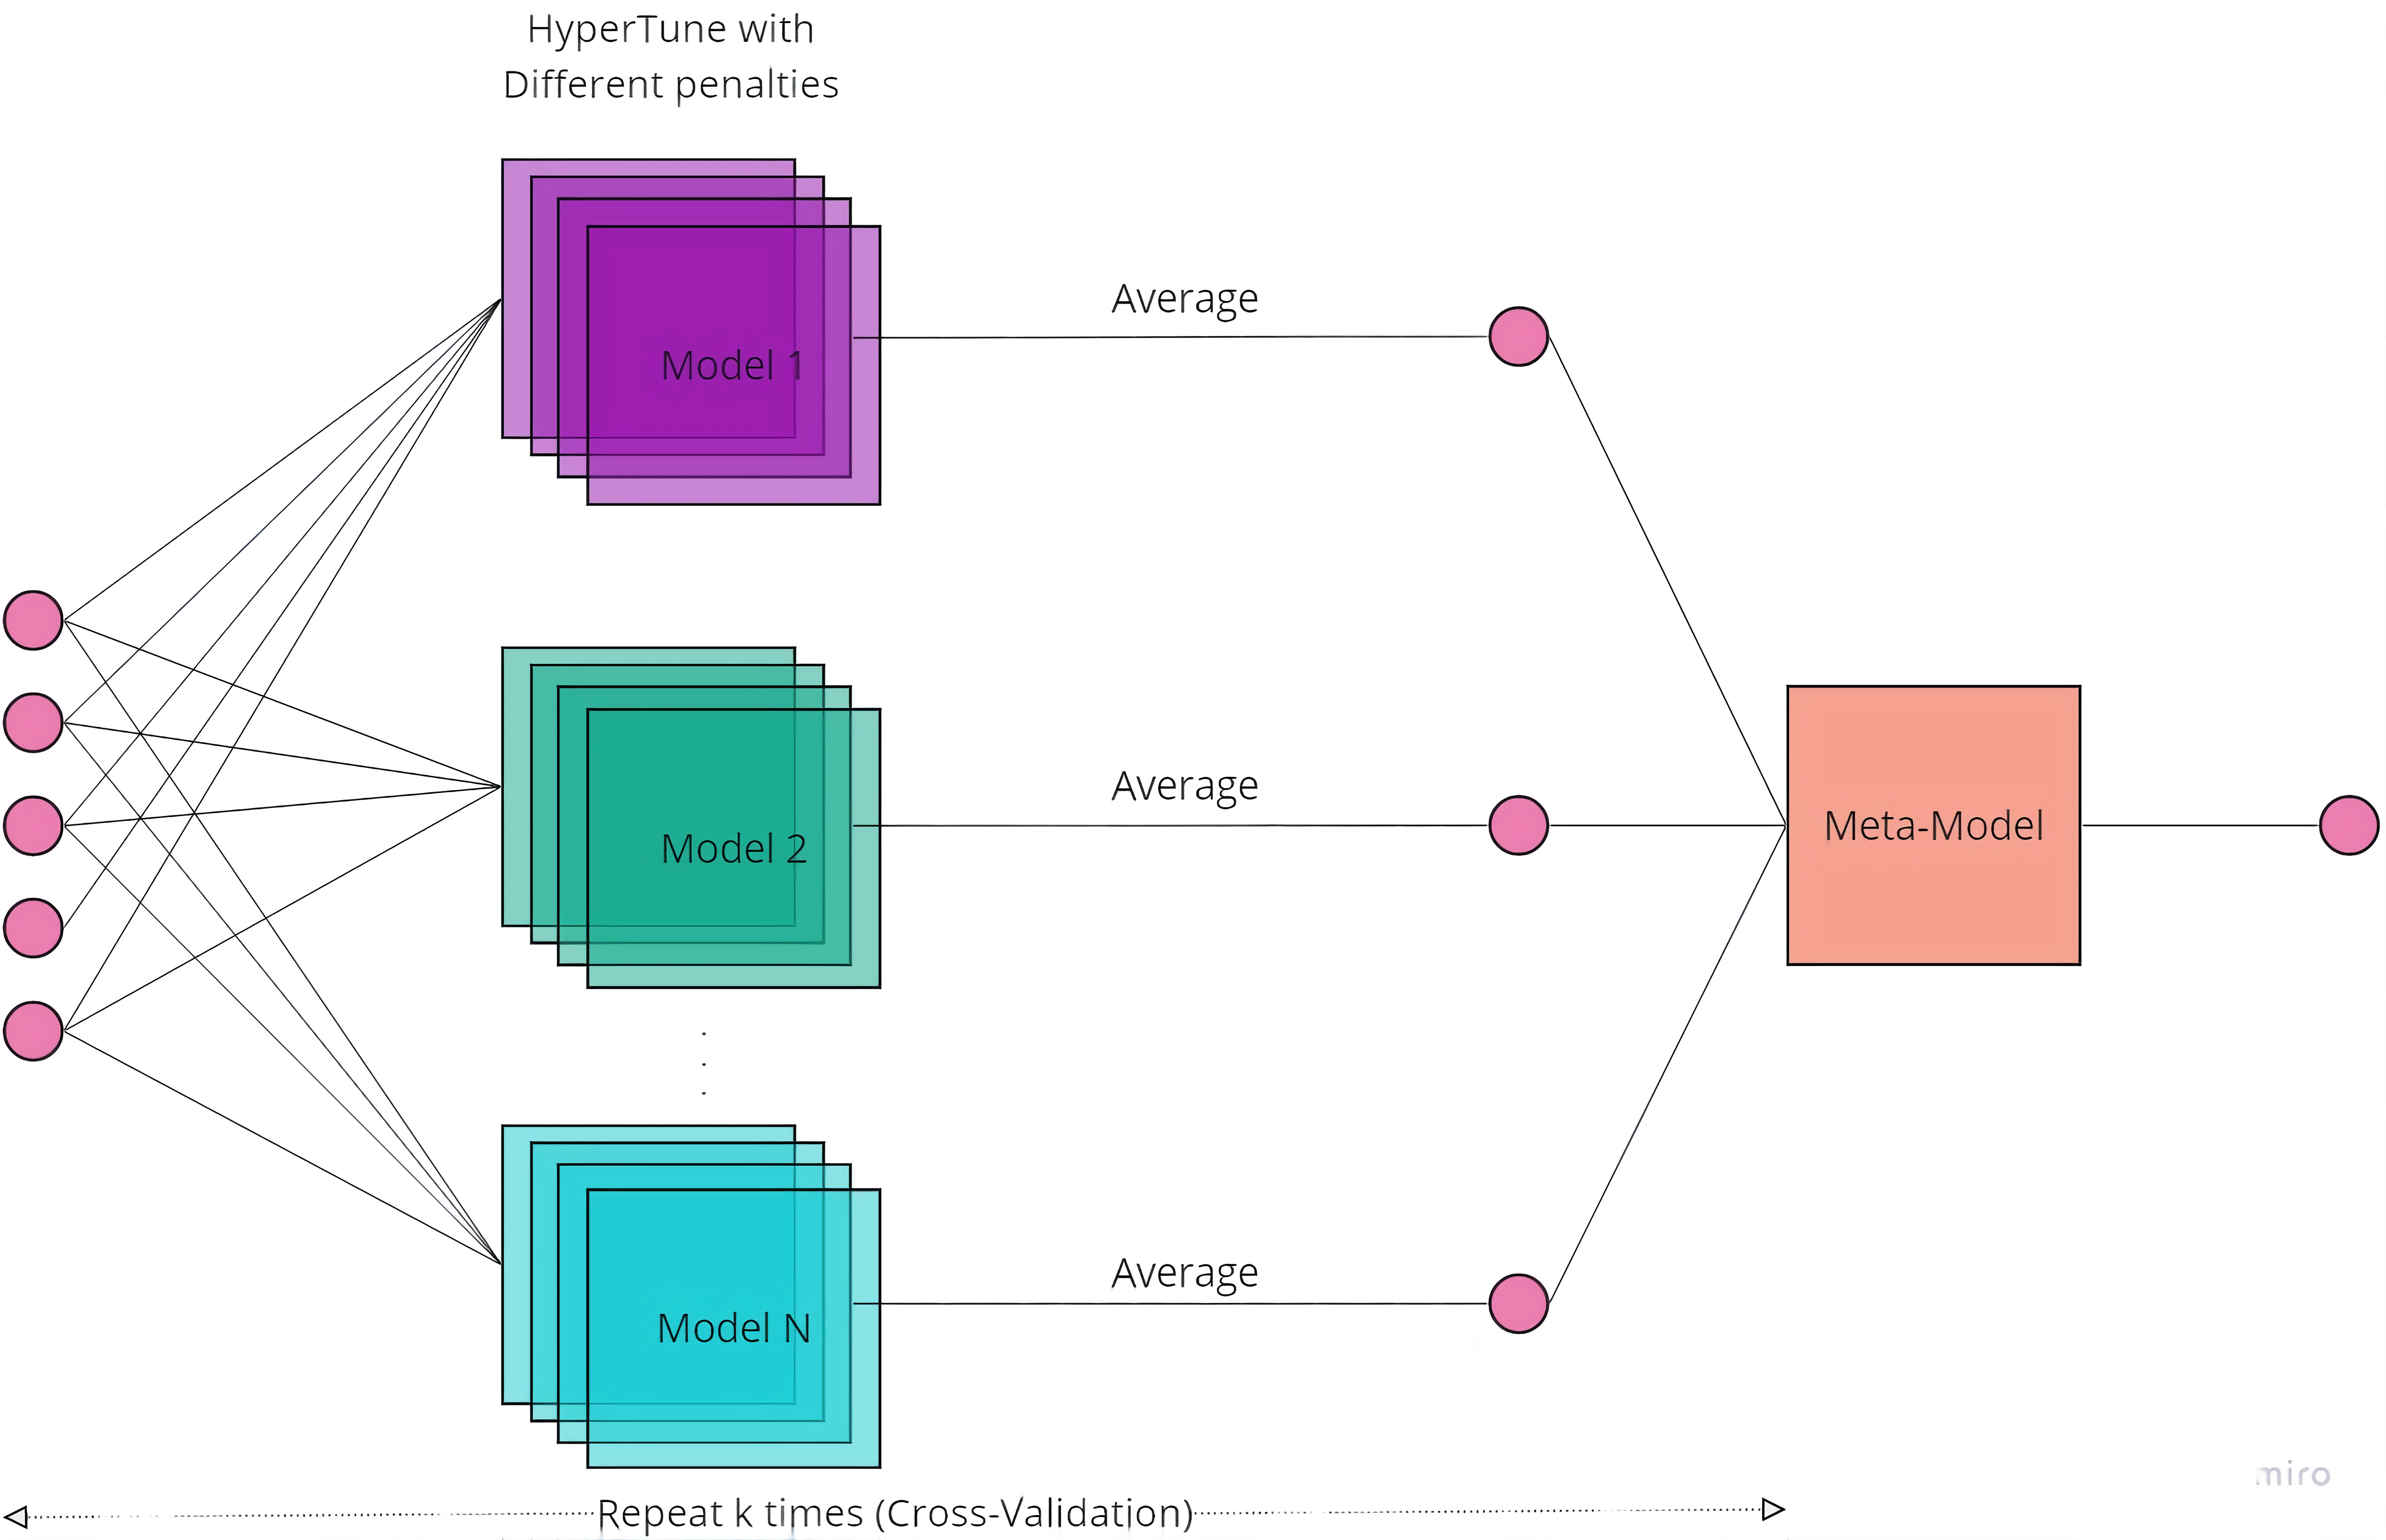
\includegraphics[width=12cm, ]{pictures/ourapproach_general.jpg}
\caption{
شمای روش پیشنهادی
}\label{wrap-fig:4}
\end{figure}
با توجه به روش ارائه شده ما مدلی بدین شکل درست کرده‌ایم:
\begin{figure}[H]
\centering
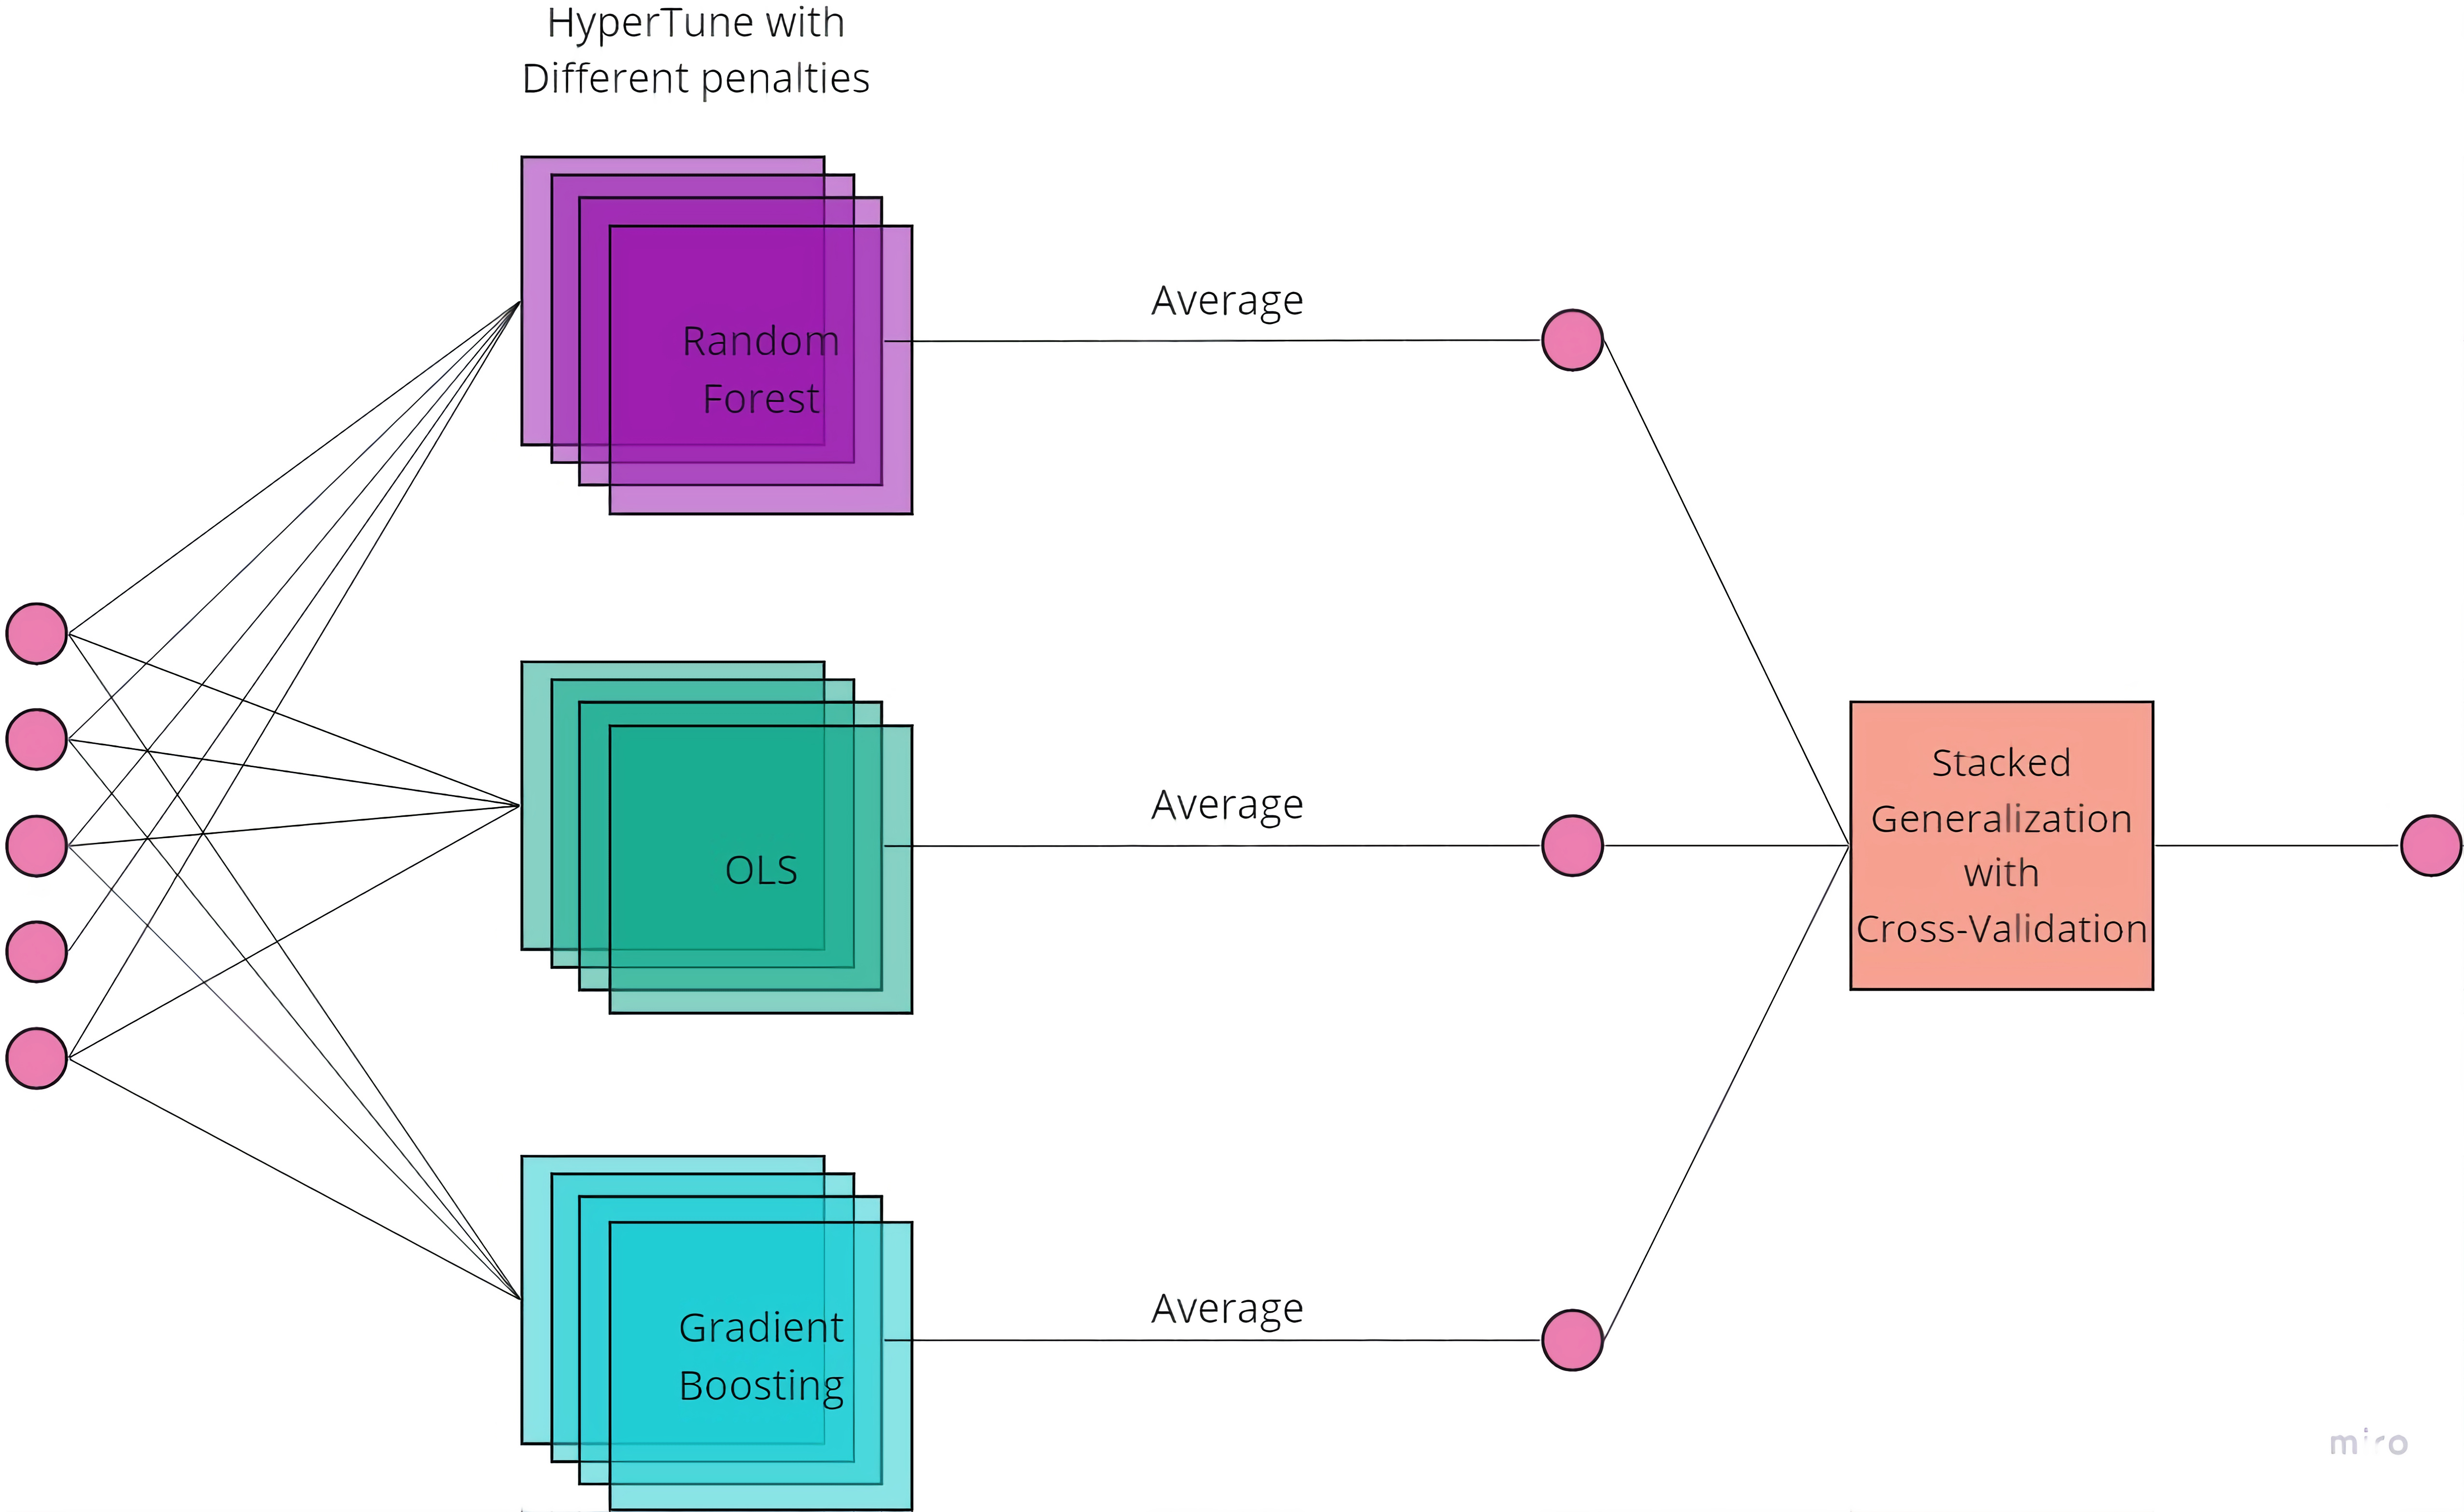
\includegraphics[width=12cm, ]{pictures/ourapproach.jpg}
\caption{
شمای دقیق استفاده شده برای بدست آوردن نتیجه
}\label{wrap-fig:4}
\end{figure}
\subsection{آنالیز مشخصات پنهان}
آنالیز مشخصات پنهان (به انگلیسی: \lr{Latent Profile Analysis}) (به اختصار LPA )، یک رویکرد مدل‌سازی آماری برای تخمین پروفایل‌های متمایز متغیرها است. در علوم اجتماعی و در تحقیقات آموزشی، این پروفایل‌ها می‌توانند به عنوان مثال نشان دهند که چگونه سن‌های مختلف در آزمایش تاثیرگذار بوده اند. توجه داشته باشید که LPA با متغیرهای پیوسته (و در برخی موارد، متغیرهای ترتیبی) کار را دارد، اما برای متغیرهای دوگانه (دودویی) مناسب نیست. ما به کمک برنامه‌ی  tidyLPA شیش مدل مختلف را تست کردیم، همانطور که قبلا هم اعلام کردیم، فرضیات LPA را در نظر نداشته‌ایم و فقط به صورت آزمایشی آن را امتحان کردیم. به طور کلی، رویکرد انتخاب مدل مشابه انتخاب تعداد پروفایل‌ها است، که مستلزم تصمیم‌گیری بر اساس شواهد از منابع متعدد، از جمله معیارهای اطلاعاتی، آزمون‌های آماری، و تفسیرپذیری است.\\

 در tidyLPA، شش مدلی که امکان تعیین آنها در LPA وجود دارد از نظر چگونگی تخمین متغیرهای مورد استفاده برای ایجاد پروفایل‌ها توضیح داده شده است.\\
 ۱. واریانس پروفایل‌ها برابر و کواریانس آنها برابر با صفر است (مدل ۱) ۲. واریانس پروفایل‌ها متفاوت و کواریانس آنها برابر با صفر است (مدل ۲) ۳. واریانس پروفایل‌ها برابر و کواریانس آنها نیز برابر است (مدل ۳) ۴. میانگین پروفایل‌ها متفاوت، واریانس آنها متفاوت و کواریانس آنها برابر است (مدل ۴) ۵. میانگین پروفایل‌ها متفاوت، واریانس آنها برابر و کواریانس آنها متفاوت است (مدل ۵) ۶. واریانس پروفایل‌ها متفاوت و کواریانس آنها متفاوت است (مدل ۶)

هنگام استفاده از پکیج tidyLPA ، کافی است مدل خود و تعداد پروفایل‌ها را انتخاب کنید و پکیج در صورت همگرا بودن جواب،‌ آن را نمایش می‌دهد، ما تمام ۶ مدل را برای دو پروفایل sgRNAهای موثر و ناموثر امتحان کردیم که فقط دو مدل جواب همگرا داشتند و آن‌ها هم مدل ۱و۲ بودند.
\section{Attention}
موفقیت ما در روش ensemble ، بر خلاف الگوریتم‌های دیگر که با استفاده از اطلاعات جانبی دیگر در مورد sgRNA بود، بر حسب نمایش دادن sgRNA در یک بردار معنادار بود. به همین جهت ما سعی کردیم که یک بردار معنادار از هر ‌sgRNA بسازیم و برای این امر از روش توجه استفاده کردیم.

در شبکه‌های عصبی، توجه تکنیکی است که توجه شناختی را تقلید می کند. این اثر باعث می‌شود که اثر برخی از بخش‌های ورودی افزایش یابد در حالی که بخش‌های دیگر را کاهش می‌دهد - فکر این است که شبکه باید تمرکز بیشتری را به آن بخش کوچک اما مهم داده اختصاص دهد. یادگیری اینکه کدام بخش از داده ها مهم تر از سایرین است بستگی به زمینه دارد و با نزول گرادیان آموزش داده می شود.

مکانیسم‌های مانند توجه در دهه 1990 با نام هایی مانند ماژول های ضربی، واحدهای سیگما پی و ابرشبکه ها معرفی شدند. ~\cite{Yann} انعطاف پذیری آن ناشی از نقش آن به عنوان "وزن نرم" است که می تواند در طول زمان اجرا تغییر کند، برخلاف وزنه های استاندارد که باید در زمان اجرا ثابت بمانند. کاربردهای توجه شامل حافظه در ماشین‌های تورینگ عصبی، وظایف استدلال در رایانه‌های عصبی متمایز ~\cite{Hybrid}، پردازش زبان در ترانسفورماتورها، و پردازش داده‌های چندحسی (صدا، تصاویر، ویدئو، متن) در درک‌کننده‌ها است.~\cite{Vaswani, Ramachandran, Jaegle, Ray} 	

این مدل‌ها از دو قسمت نظارت شده و  نظارت نشده تشکیل شده که اولین آموزش برای پیدا کردن ساختار کلی است و دومین آموزش برای تنظیم مناسب برای امر خاص است.

در اینجا ما چند مدل مختلف مانند bert و roberta و DNAbert \cite{DNABERT} برای کلاس بندی sgRNAها استفاده کردیم که نتایج این مدل‌ها خیلی ضعیف بود. با توجه به آنالیزهای انجام شده به این نتیجه رسیدیم که مشکل از دیتاهای بدون برچسپ و برچسب زده استفاده شده در طول آموزش‌ها بود. برای ساخت token ابتدا از روش مرسوم kmer در دی‌ان‌ای استفاده کردیم که به این صورت است که برای هر حرف از توالی k حرف بعد از آن تکرار می‌شود. سپس این کلمات kتایی را به عنوان دیکشنری کلمات در نظر می گیریم. برای قسمت pretrain از sgRNA که خودمان ذخیره کرده بودیم و داده‌های دیگر استفاده کردیم و سپس برای تنظیمات نهایی از داده‌های مقاله DNAbert استفاده کردیم ولی نتایج آن نتایج جالبی نبود.
\begin{figure}
\centering
\includegraphics[width=10cm, ]{pictures/dnabert.jpg}
\caption{
مدل دقت DNAbert \cite{DNABERT}
}\label{wrap-fig:4}
\end{figure}



با توجه به پژوهش‌های انجام شده، به صورت جداگانه موفق به ارائه روشی مناسب برای حل مسئله نشده‌ایم، این امر به دلیل وجود نویز در داده به خاطر کم بودن ویژگی‌های مدل و تعداد کم داده‌های برچسب زده بود ولی با استفاده از کار پیشین و استفاده از تجربه آموزش مدل‌های دیگر روی تعداد داده بیشتر و ویژگی‌های بیشتر توانستیم روشی ارائه کنیم که عمومی‌تر و دقیق‌تر باشد.
\chapter{نتایج شبیه‌سازی}
ابتدا نمایشی از داده‌های گلدن استاندارد و تفاوت آنها در آزمایش‌ها مختلف را نشان می دهیم:
\begin{table}[!ht]

    \caption{ تفاوت اندازه‌گیری فرکانس ایندل‌ها برای یک سل‌لاین در دو پژوهش مختلف}
\begin{latin}
\begin{tabularx}{\textwidth}{|l|Y|Y|}
\hline
\rowcolor{Goldenrod}	
\multicolumn{3}{|c|}{Wang et al. (2019) \cite{Wang}  – Kim et al. (2019) \cite{Kim} } \\ \hline 
\rowcolor{Goldenrod}	
	gRNA+PAM & Wang et al. (2019)
Indel\_freq\_HEK293T & Kim et al. (2019)
Indel\_freq\_HEK293T \\ \hline
	GAGGAAGCAGATATCCGGTGTGG & 94.313725490196006 & 40.490007577838398 \\ \hline
	GGAGGAGGCTGAACGCACGAGGG & 90.129016553067203 & 74.369471837500697 \\ \hline
	GCTGCGAGACCGCTATCCCGTGG & 94.1153758800817 & 85.4296388542964 \\ \hline
	GCGCGTCGAACACGAACCAGCGG & 94.067796610169395 & 61.945179048985402 \\ \hline
	ATACTCACATCACAGCCCGCTGG & 45.164998674709402 & 43.601387998980698 \\ \hline
	GACTACGCCTCTGCCTTTCAAGG & 42.752196781612703 & 24.8797250859107 \\ \hline
	GACAGTGCGCACCGTGTACGTGG & 86.950586950586896 & 87.678945915304297 \\ \hline
	GTCCCAACTCCTGCGCACGAAGG & 87.792680154580495 & 78.251019483461704 \\ \hline
	GTATGTCGAGAGTACCAACGTGG & 93.989694643289397 & 84.282105733435799 \\ \hline
	GAAGTCCCGAATGACTCCTGTGG & 95.953478478770094 & 51.447561838907902 \\ \hline
	GCAAGAGCTCTCAATTACACAGG & 26.400666586386201 & 41.090027521361897 \\ \hline
	GACCTACCACCGAGCCATCAAGG & 45.699392752721998 & 48.920244981226801 \\ \hline
	ATTCTTACAGACAGGTCCGGTGG & 71.398959583833502 & 58.898283855940598 \\ \hline
	ATTCCAGATCCAAGTGCGAAAGG & 19.416422401075099 & 30.0529172782263 \\ \hline
	ATAACCTGTAAGCCCCACAAAGG & 84.049773755656105 & 72.983725135623899 \\ \hline
	GAGCATGCCAGCACGCTCAAGGG & 35.8299328682374 & 68.013567829869004 \\ \hline
	GGAAGCCGAGATCCCCCGCGAGG & 96.926026719445801 & 50.104123281965897 \\ \hline
	GGTCCCCTTAGCTCTCATGTTGG & 65.196962505932603 & 60.4208849810732 \\ \hline
	GGACCGGGAAGCAATTCGACAGG & 60.6481507594943 & 48.141659670510599 \\ \hline
	AGCGTAAGCCAATACTGATGAGG & 60.069097691358699 & 58.825459317585299 \\ \hline
	GCTTCCAAGTAGCACTCAGTAGG & 50.230952263469199 & 43.932746018438102 \\ \hline
	GCTGCACTACTACCCGCACGTGG & 88.571428571428498 & 70.507599887110402 \\ \hline
	AAATCTTGTGAACCTCATCGAGG & 76.194029850746205 & 42.066691095639399 \\ \hline
\end{tabularx}
\end{latin}
\end{table}


در اینجا ما از داده‌های ارائه شده در مقاله DeepCRISPR برای مقایسه مدل‌های مختلف استفاده کرده‌ایم که حدود ۴۳۰ دنباله دی‌ان‌ای و نتیجه پیش‌بینی ۵ الگوریتم مختلف بود است، برای انجام آزمایش، ۸۰٪ داده‌ها را برای آموزش و ۲۰٪ داد‌ه‌ها را برای تست استفاده کرده‌ایم.
\begin{table}[H]

    \caption{ داده‌های مقایسه امتیاز الگوریتم‌های مختلف \cite{DeepCRISPR}}
\begin{latin}
\begin{adjustbox}{center}
\resizebox{1.2\columnwidth}{!}{%
\begin{tabularx}{2.08\textwidth}{|l|c|c|c|c|c|c|c|c|}
\hline \hline
\rowcolor{Goldenrod}	
	sgRNA number & KO reporter assay & DeepCRISPR score & CRISPRater score & SSC Score & sgRNA Scorer score & sgRNA Designer rsII score & sgRNA sequence & extended spacer \\ \hline
	sg1 & 0 & 0.17706534 & 0.571 & -0.485 & 30.66 & 0.571 & GAGTCGGGGTTTCGTCATGTTGG & AGTAGAGTCGGGGTTTCGTCATGTTGGTCA \\ \hline
	sg2 & 0 & 0.055156678 & 0.6998 & -0.266 & 54.96 & 0.533 & CGCCGCCGCTTTCGGTGATGAGG & CTGCCGCCGCCGCTTTCGGTGATGAGGAAA \\ \hline
	sg3 & 0 & 0.23954645 & 0.6865 & -0.448 & 25.79 & 0.41 & GGCAGCGTCGTGCACGGGTCGGG & CCCGGGCAGCGTCGTGCACGGGTCGGGTGA \\ \hline
	sg4 & 0 & 0.147778 & 0.6405 & -4.6E-2 & 53.81 & 0.491 & TGGGCGGATCACTTGACGTCAGG & GAGGTGGGCGGATCACTTGACGTCAGGAGT \\ \hline
	sg5 & 0 & 0.121 & 0.68 & 6.7E-2 & 12.44 & 0.485 & TTACCATAGTGTACGGGTGCAGG & CTTTTTACCATAGTGTACGGGTGCAGGCAT \\ \hline
	sg6 & 0 & 0.14186779 & 0.5489 & 0.085 & 64.75 & 0.489 & TCTACTGAAGTGGTAGCAACAGG & TTCTTCTACTGAAGTGGTAGCAACAGGTAC \\ \hline
	sg7 & 0 & 0.10871141 & 0.6207 & 0.107 & 24.01 & 0.554 & TAGAGATCCGCCCTATCTCAAGG & CAGATAGAGATCCGCCCTATCTCAAGGGAC \\ \hline
	sg8 & 0 & 0.14419994 & 0.6916 & 0.91 & 73 & 0.448 & CTCATCACCGAAAGCGGCGGCGG & TTTCCTCATCACCGAAAGCGGCGGCGGCAG \\ \hline
	sg9 & 0.028 & 0.11949389 & 0.5259 & -0.578 & 9.73 & 0.441 & TTCTGAATTATCGGCTAGCCTGG & AGATTTCTGAATTATCGGCTAGCCTGGTCT \\ \hline
	sg10 & 0.036 & 0.151749 & 0.4501 & -0.329 & 52.9 & 0.412 & GCCTCAGCCTCACGAATAGCTGG & GCCTGCCTCAGCCTCACGAATAGCTGGGAT \\ \hline
	sg11 & 0.037 & 0.13260305 & 0.5663 & -0.364 & 10.57 & 0.521 & AAGTACTCCTGGAGTACTGCAGG & CCCAAAGTACTCCTGGAGTACTGCAGGAGG \\ \hline
	sg12 & 0.056 & 0.28234875 & 0.7611 & 0.019 & 83.17 & 0.624 & CACCGTAGTCAATCTCAATGAGG & AGATCACCGTAGTCAATCTCAATGAGGGCC \\ \hline
	sg13 & 0.064 & 0.099274084 & 0.6184 & 0.318 & 15.79 & 0.504 & ACGGAGTCTCGCTGTCGCCCAGG & TGAGACGGAGTCTCGCTGTCGCCCAGGCTG \\ \hline
	sg14 & 0.066 & 0.14608404 & 0.6311 & 0.002 & 51.42 & 0.395 & TGGGATGCCGTCCCGCAAAATGG & GTAGTGGGATGCCGTCCCGCAAAATGGCCC \\ \hline
	sg15 & 0.072 & 0.098504 & 0.6751 & 0.587 & 79.21 & 0.599& TCCGAGAGAAACCTTCGCAAGGG & CAGATCCGAGAGAAACCTTCGCAAGGGATT \\ \hline
	sg16 & 0.109 & 0.14631987 & 0.5128 & -0.327 & 55.6 & 0.27399 & CCGTCCAGCCACGGCAAGCCTGG & GCCCCCGTCCAGCCACGGCAAGCCTGGGCT \\ \hline
	sg17 & 0.111 & 0.19384801 & 0.8201 & -0.249 & 22.99 & 0.505 & CTAGTGGAAGTGAACGCTCCTGG & TGGACTAGTGGAAGTGAACGCTCCTGGCAT \\ \hline
	sg18 & 0.113 & 0.20544451 & 0.5886 & -0.102 & 43.12 & 0.561 & GGGCATATGGACTAGGCACTGGG & TGTGGGGCATATGGACTAGGCACTGGGCTA \\ \hline
	sg19 & 0.125 & 0.097481444 & 0.6024 & -0.278 & 3.89 & 0.438 & TGACATTTCAATTCCGTAGCTGG & ACACTGACATTTCAATTCCGTAGCTGGACA \\ \hline
	sg20 & 0.137 & 0.24448508 & 0.6321 & 0.374 & 78.21 & 0.661& GCTTACCAGTATGACGACGATGG & GTGTGCTTACCAGTATGACGACGATGGGTA \\ \hline
	sg21 & 0.14 & 0.17448096 & 0.7384 & 1.44 & 97.25 & 0.718 & GTTCAGGAATCGTCACCCGGCGG & CGCGGTTCAGGAATCGTCACCCGGCGGCCT \\ \hline
	sg22 & 0.156 & 0.19983143 & 0.6321 & 0.013 & 45.91 & 0.521 & GCTAACGATCTCTTTGATGATGG & TTCTGCTAACGATCTCTTTGATGATGGCTG \\ \hline
	sg23 & 0.161 & 0.18330452 & 0.6786 & 0.155 & 24.17 & 0.425 & ACCAGTTCACAAACGGGCCTCGG & TCCCACCAGTTCACAAACGGGCCTCGGGCT \\ \hline
	sg24 & 0.162 & 0.1040944 & 0.4028 & -0.512 & 30.01 & 0.393 & AGCTACCAGGCTAGAGTGCCAGG & AAGCAGCTACCAGGCTAGAGTGCCAGGCAT \\ \hline
	sg25 & 0.179 & 0.16135208 & 0.6374 & -0.241 & 49.36 & 0.215 & TCGGCTGGAAATATGTTTAAAGG & TCTATCGGCTGGAAATATGTTTAAAGGATT \\ \hline
\end{tabularx}}
\end{adjustbox}
\end{latin}
\end{table}
\section{LPA}
اولین آزمایشی که در روش LPA انجام دادیم این بود که ببینیم کدام یک از مدل‌ها همگرا می‌شوند:
\begin{table}[H]

    \caption{ نتیجه اجرای مدل‌های مختلف بر تقسیم به ۳ یا ۲ پروفایل}
\begin{latin}
\begin{adjustbox}{center}
\resizebox{1.2\columnwidth}{!}{%
\begin{tabularx}{1.796\textwidth}{|c|c|c|c|c|c|c|c|c|c|c|c|c|c|c|c|c|c|}
\hline 
\rowcolor{YellowGreen} 
	Model & Classes & LogLik & AIC & AWE & BIC & CAIC & CLC & KIC & SABIC & ICL & Entropy & prob\_min & prob\_max & n\_min & n\_max & BLRT\_val & BLRT\_p \\ \hline
1 & 2 & -2787.420 & 5606.840 & 5814.917 & 5671.673 & 5687.673 & 5576.430 & 5625.840 & 5620.900 & -5730.746 & 0.795 & 0.937 & 0.944 & 0.44471 & 0.55529 & 450.642 & 0 \\ \hline
1 & 3 & -2759.128 & 5562.256 & 5849.152 & 5651.402 & 5673.402 & 5519.652 & 5587.256 & 5581.588 & -5793.690 & 0.698 & 0.795 & 0.895 & 0.28706 & 0.36941 & 56.585 & 0 \\ \hline
5 & 2 & {\color{gray} NA} & {\color{gray} NA} & {\color{gray} NA} & {\color{gray} NA} &{\color{gray} NA} & {\color{gray} NA} & {\color{gray} NA} & {\color{gray} NA} & {\color{gray} NA} & {\color{gray} NA} & {\color{gray} NA} & {\color{gray} NA} & {\color{gray} NA} & {\color{gray} NA} & {\color{gray} NA} & {\color{gray} NA} \\ \hline
5 & 3 & {\color{gray} NA} & {\color{gray} NA} & {\color{gray} NA} & {\color{gray} NA} &{\color{gray} NA} & {\color{gray} NA} & {\color{gray} NA} & {\color{gray} NA} & {\color{gray} NA} & {\color{gray} NA} & {\color{gray} NA} & {\color{gray} NA} & {\color{gray} NA} & {\color{gray} NA} & {\color{gray} NA} & {\color{gray} NA} \\ \hline
3 & 2 & {\color{gray} NA} & {\color{gray} NA} & {\color{gray} NA} & {\color{gray} NA} &{\color{gray} NA} & {\color{gray} NA} & {\color{gray} NA} & {\color{gray} NA} & {\color{gray} NA} & {\color{gray} NA} & {\color{gray} NA} & {\color{gray} NA} & {\color{gray} NA} & {\color{gray} NA} & {\color{gray} NA} & {\color{gray} NA} \\ \hline
3 & 3 & {\color{gray} NA} & {\color{gray} NA} & {\color{gray} NA} & {\color{gray} NA} &{\color{gray} NA} & {\color{gray} NA} & {\color{gray} NA} & {\color{gray} NA} & {\color{gray} NA} & {\color{gray} NA} & {\color{gray} NA} & {\color{gray} NA} & {\color{gray} NA} & {\color{gray} NA} & {\color{gray} NA}& {\color{gray} NA} \\ \hline
2 & 2 & -2777.674 & 5597.348 & 5870.764 & 5682.442 & 5703.442 & 5557.120 & 5621.348 & 5615.801 & -5713.236 & 0.886 & 0.947 & 0.977 & 0.27765 & 0.72235 & 470.136 & 0  \\ \hline
2 & 3 & -2706.045 & 5476.090 & 5893.834 & 5605.757 & 5637.757 & 5413.680 & 5511.090 & 5504.209 & -5701.814 & 0.795 & 0.890 & 0.939 & 0.21176 & 0.50824 & 143.589 & 0 \\ \hline
6 & 2 & {\color{gray} NA} & {\color{gray} NA} & {\color{gray} NA} & {\color{gray} NA} &{\color{gray} NA} & {\color{gray} NA} & {\color{gray} NA} & {\color{gray} NA} & {\color{gray} NA} & {\color{gray} NA} & {\color{gray} NA} & {\color{gray} NA} & {\color{gray} NA} & {\color{gray} NA} & {\color{gray} NA} & {\color{gray} NA} \\ \hline
6 & 3 & {\color{gray} NA} & {\color{gray} NA} & {\color{gray} NA} & {\color{gray} NA} &{\color{gray} NA} & {\color{gray} NA} & {\color{gray} NA} & {\color{gray} NA} & {\color{gray} NA} & {\color{gray} NA} & {\color{gray} NA} & {\color{gray} NA} & {\color{gray} NA} & {\color{gray} NA} & {\color{gray} NA} & {\color{gray} NA} \\ \hline
4 & 2 & {\color{gray} NA} & {\color{gray} NA} & {\color{gray} NA} & {\color{gray} NA} &{\color{gray} NA} & {\color{gray} NA} & {\color{gray} NA} & {\color{gray} NA} & {\color{gray} NA} & {\color{gray} NA} & {\color{gray} NA} & {\color{gray} NA} & {\color{gray} NA} & {\color{gray} NA} & {\color{gray} NA} & {\color{gray} NA} \\ \hline
4 & 3 & {\color{gray} NA} & {\color{gray} NA} & {\color{gray} NA} & {\color{gray} NA} &{\color{gray} NA} & {\color{gray} NA} & {\color{gray} NA} & {\color{gray} NA} & {\color{gray} NA} & {\color{gray} NA} & {\color{gray} NA} & {\color{gray} NA} & {\color{gray} NA} & {\color{gray} NA} & {\color{gray} NA} & {\color{gray} NA} \\ \hline
\end{tabularx}}
\end{adjustbox}
\end{latin}
\end{table}

\begin{figure}[H]
\centering
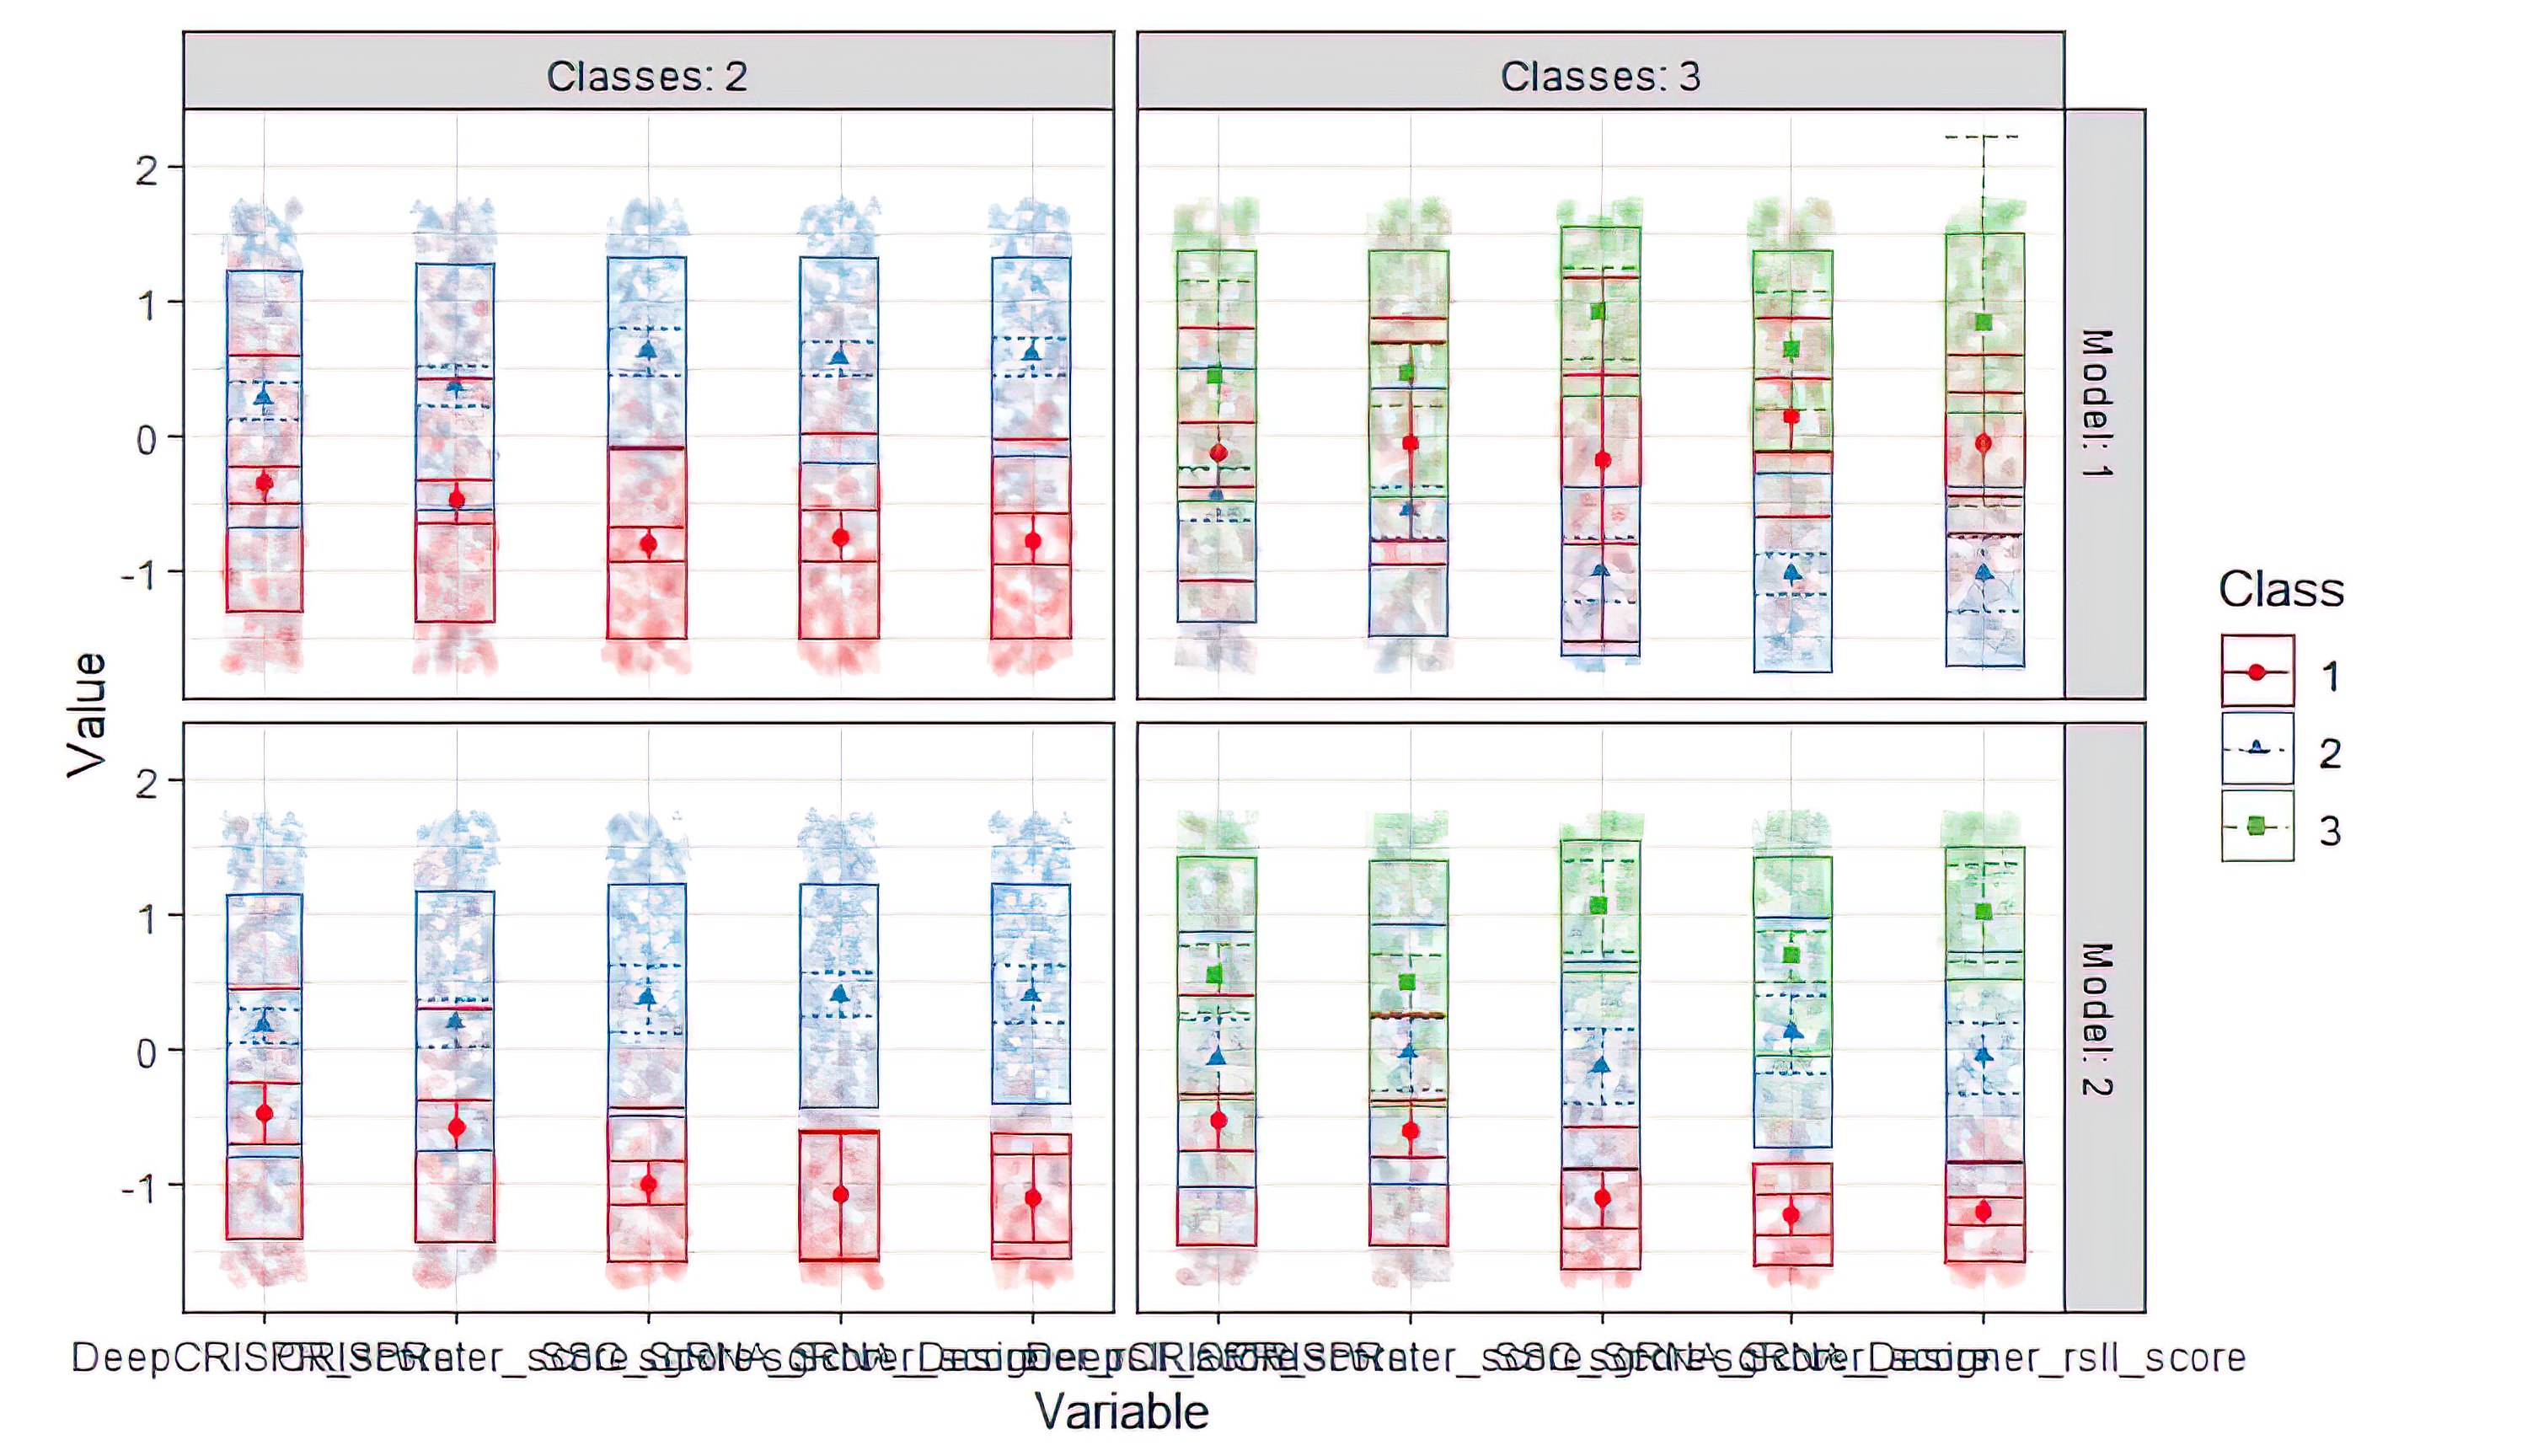
\includegraphics[width=12cm, ]{pictures/tidyLPA.jpg}
\caption{
پراکندگی داده نسبت به کلاس‌ها
}\label{wrap-fig:4}
\end{figure}

مقایسه این مدل‌ها با کار‌های پیشین نشان داد که روش قابل قبول نیست.
\begin{table}[H]

    \caption{ داده‌های مقایسه امتیاز الگوریتم‌های مختلف \cite{DeepCRISPR}}
\begin{latin}
\begin{adjustbox}{center}
\resizebox{1\columnwidth}{!}{%
\begin{tabularx}{1.072\textwidth}{|l|c|c|c|c|c|c|c|}
\hline 
\rowcolor{YellowGreen} 
	& Model 1 & *Ours & DeepCrispr & CRISPRater & SSC & sgRNA Scorer & sgRNA Scorer  \\ \hline
\rowcolor{SeaGreen}\multicolumn{8}{|c|}{Thershold = 0.6} \\ \hline
Accuracy Score: & 0.648140 & 0.914763 & 0.739884 & 0.660604 & 0.586359 & 0.580693 & 0.598542\\ \hline
Precision Recall Score: & 0.715779 & 0.936461 & 0.807515 & 0.714867 & 0.648901 & 0.662849 & 0.673465 \\ \hline
F1 Score: &  0.557377 & 0.875740 & 0.0 & 0.541463 & 0.159468 & 0.762044 & 0.078571\\ \hline
\rowcolor{SeaGreen}\multicolumn{8}{|c|}{Thershold = 0.7} \\ \hline
Accuracy Score:& 0.631560 & 0.880356 & 0.684054 & 0.642937 & 0.563159 & 0.568745 & 0.623188 \\
Precision Recall Score: & 0.531786 & 0.823824 & 0.581910 & 0.520233 & 0.440453 & 0.476842 & 0.494809 \\ \hline
F1 Score: & 0.489297 & 0.712329 & 0.0 & 0.167488 & 0.108911 & 0.579564 & 0.0 \\ \hline
\rowcolor{SeaGreen}\multicolumn{8}{|c|}{Thershold = 0.8} \\ \hline
Accuracy Score:& 0.521924 & 0.830463 & 0.635765 & 0.608747 & 0.427671 & 0.475937 & 0.585022 \\
Precision Recall Score: & 0.185667 & 0.503301 & 0.168832 & 0.148355 & 0.091240 & 0.107466 & 0.179785\\ \hline
F1 Score: & 0.171123 & 0.156863 & 0.0 & 0.0 & 0.0& 0.2 & 0.0 \\ \hline
\end{tabularx}}
\end{adjustbox}
\end{latin}
\end{table}

شایان ذکر است که چون در روش LPA از کل داده‌ها برای آموزش استفاده می‌شود، برای حساب کردن امتیاز سایر الگوریتم‌ها نیز از کل داده استفاده کردیم و از آنجا که روش پیشنهادی \lr{(*Ours)} نیز با همین داده‌ها آموزش داده شده پس این مقایسه، مقایسه‌ی خوبی برای بررسی توانایی روش پیشنهادی نیست.

\section{روش پیشنهادی}
  نمونه‌ای از نتایج اولیه استفاده مستقیم روش‌های LPA و رگرسیون برای پیدا کردن وزن خوب بین اکسپرت‌ها با استفاده از کل داده‌ها با threshold های مختلف (کلاس‌بندی).

حال نتیجه روش‌ پیشنهادی برای ادغام متد‌های پیشین که با تقسیم ۷۰ به ۳۰ بدست آمده است و برای مقایسه رگرسیون آنها از رابطه اسپیرمن بین پیش‌بینی‌ها و داده واقعی و مربع تفاضلات میانگین استفاده کرده‌ایم. این روش را روی 100 تقسیم تصادفی امتحان کرده‌ایم و میانگین هر کدام را ارائه می‌دهیم:
\begin{table}[H]

    \caption{مقایسه کامل روش DeepCRISPR با روش‌های مختلف Ensemble}
\begin{latin}
\begin{adjustbox}{center}
\resizebox{1.2\columnwidth}{!}{%
\begin{tabularx}{2.13\textwidth}{| l | c | c | c | c | c | c | c | c | }
\hline
	\rowcolor{SeaGreen}\multicolumn{9}{|c|}{Regression} \\ \hline
	& *OURS & DeepCRISPR & RandomForest & LinearRegression	 & GradientBoosting 	 & Average RandomForestRegressor & Average LinearRegression & Average GradientBoosting \\ \hline
	spearman\_score & 0.48363014255265202 & 0.44920573337131903 & 0.442334582432172 & 0.48875954923704201 & 0.42820701429086999 & 0.445627937403689 & 0.486785109490944 & 0.43753255749096398 \\ \hline
	MSE\_score & 4.3495596387515302E-2 & 8.8698237964087503E-2 & 4.07988086339467E-2 & 4.4421889409931303E-2 & 4.2615593436146702E-2 & 5.77039089254009E-2 & 4.5011123276089499E-2 & 5.0119844259733599E-2 \\ \hline
	\  & \  & \  & \  & \  & \  & \  & \  & \  \\ \hline
	\rowcolor{SeaGreen}\multicolumn{9}{|c|}{Classification}  \\ \hline
	Thershold: 0.7 & *OURS & DeepCRISPR & RandomForest & LinearRegression	 & GradientBoosting 	 & Average RandomForestRegressor & Average LinearRegression & Average GradientBoosting \\ \hline
	accuracy\_score & 0.65585937500000002 & 0.53796875 & 0.677734375 & 0.645390625 & 0.69515625000000003 & 0.67257812500000003 & 0.64156250000000004 & 0.61054687500000004 \\ \hline
	roc\_auc\_score & 0.66431776673864995 & 0.61734640570578403 & 0.65843505577961503 & 0.65901999368111197 & 0.67276455067103103 & 0.65458082510786497 & 0.658802600125869 & 0.63919789305687402 \\ \hline
	precision\_score & 0.792557700213534 & 0.85072046233693299 & 0.76624039613931905 & 0.79259641935763803 & 0.77357966284998403 & 0.76411257617980399 & 0.79565743804489097 & 0.79178486827439998 \\ \hline
	recall\_score & 0.63734210988092399 & 0.34806419545723799 & 0.72518684127973998 & 0.614432263387238 & 0.74964082726952797 & 0.71661369491892901 & 0.60264418676158005 & 0.55093050984697001 \\ \hline
	f1\_score & 0.703752997266619 & 0.49253449071580302 & 0.74347366186999897 & 0.690397602288365 & 0.76016707914694104 & 0.73783309071755199 & 0.68385488400419403 & 0.64166082655091905 \\ \hline
	\  & \  & \  & \  & \  & \  & \  & \  & \  \\ \hline
	\rowcolor{SeaGreen}\multicolumn{9}{|c|}{Classification}  \\ \hline
	Thershold: 0.8 & *OURS & DeepCRISPR & RandomForest & LinearRegression	 & GradientBoosting 	 & Average RandomForestRegressor & Average LinearRegression & Average GradientBoosting \\ \hline
	accuracy\_score & 0.62843749999999898 & 0.60109374999999898 & 0.60835937500000004 & 0.63249999999999895 & 0.61617187500000004 & 0.53515625 & 0.63835937499999895 & 0.53507812499999896 \\ \hline
	roc\_auc\_score & 0.61123631849945304 & 0.57763471246611797 & 0.59211535894568601 & 0.61618250051450296 & 0.60167042790898995 & 0.50032965589703104 & 0.622627094031456 & 0.5 \\ \hline
	precision\_score & 0.61123631849945304 & 0.70734574295302999 & 0.64704790528634304 & 0.693222291365585 & 0.64869297561177897 & 5.4545454545454498E-3 & 0.69750961557772995 & 0 \\ \hline
	recall\_score & 0.61123631849945304 & 0.24286032851065301 & 0.35517924784142701 & 0.38067809464656399 & 0.38781860176996902 & 1.2765957446808499E-3 & 0.39614240212076302 & 0 \\ \hline
	f1\_score & 0.61123631849945304 & 0.35955398993128102 & 0.45563124591441601 & 0.48885398051706602 & 0.48211167798519799 & 2.0689655172413798E-3 & 0.50302048323802395 & 0 \\ \hline
	\  & \  & \  & \  & \  & \  & \  & \  & \  \\ \hline
	\rowcolor{SeaGreen}\multicolumn{9}{|c|}{Classification}  \\ \hline
	Thershold: 0.9 & *OURS & DeepCRISPR & RandomForest & LinearRegression	 & GradientBoosting 	 & Average RandomForestRegressor & Average LinearRegression & Average GradientBoosting \\ \hline
	accuracy\_score & 0.80203124999999897 & 0.77585937500000002 & 0.80976562500000004 & 0.80156249999999896 & 0.80390625000000004 & 0.80718749999999895 & 0.79328125000000005 & 0.80718749999999895 \\ \hline
	roc\_auc\_score & 0.56430742251440802 & 0.50133606125879804 & 0.51214587901508801 & 0.57024648886899598 & 0.51169322503973103 & 0.5 & 0.59023109127478102 & 0.5 \\ \hline
	precision\_score & 0.46911614774114702 & 0.20470057720057699 & 0.411333333333333 & 0.46759052059051998 & 0.34830555555555498 & 0 & 0.44165478011840198 & 0 \\ \hline
	recall\_score & 0.17702155764350999 & 5.4478758121587097E-2 & 2.7348192951095199E-2 & 0.193655913131485 & 3.5731627260006601E-2 & 0 & 0.25916550040003999 & 0 \\ \hline
	f1\_score & 0.24884028248654999 & 8.40075202678989E-2 & 5.0123824028299999E-2 & 0.26732121294272798 & 6.2823477586924303E-2 & 0 & 0.32175545861810201 & 0 \\ \hline
\end{tabularx}}
\end{adjustbox}
\end{latin}
\end{table}
\subsection{Attention}
برای روش‌هایی که فقط از دنباله sgRNA استفاده می‌کنیم، ابتدا حدود ۴ میلیون sgRNA از دادگان کار‌های پیشین و ژن‌های مختلف جمع‌آوری کردیم و با ترنسفورمر‌های تک حرفی و چندحرفی‌ای آن‌ها را توکنایزد کردیم، همچین از مدل از پیش‌آموزش شده روی DNA و مدل بدون آموزش قبلی برای آموزش مدل‌های bert استفاده کردیم و بردار بدست‌آمده را بروی دیتا با تقسیم ۸۰ به ۲۰ و threshold ۰.۷ کلاس‌بندی کردیم.
نتیجه‌ی دسته بندی بعد از آموزش به کمک مدل‌های توجه
\begin{table}[H]
\begin{latin}
\begin{adjustbox}{center}
\resizebox{1\columnwidth}{!}{%
\begin{tabularx}{0.735\textwidth}{| l | c | c | c | }
\hline
	\rowcolor{SeaGreen}\multicolumn{4}{|c|}{DNAbert Attention Model}  \\ \hline
	& 3mer & 4mer & 6mer \  \\ \hline
	Accuracy & 0.709879518072289 & 0.709879518072289 & 0.709879518072289 \\ \hline
	AUC & 0.50249169435215901 & 0.503859617071856 & 0.503859617071856 \\ \hline
	F1 & 0.41516347237880402 & 0.41516347237880402 & 0.41516347237880402 \\ \hline
	MCC & 0 & 0 & 0 \\ \hline
	Percision & 0.35493975903609998 & 0.35493975903000002 & 0.354939759036144 \\ \hline
	Recall & 0.5 & 0.5 & 0.5 \\ \hline
\end{tabularx}}
\end{adjustbox}
\end{latin}
\caption{نتیجه‌ی آموزش مدل‌های DNAbert برای کلاس‌بندی sgRNAهای موثر و ناموثر }
\end{table}

نتیجه آموزش مدل توجه برای بدست‌آوردن بردار کد
\begin{table}[H]
\begin{latin}
\begin{adjustbox}{center}
\resizebox{0.7\columnwidth}{!}{%
\begin{tabularx}{0.585\textwidth}{| l | c | c | c | }
\hline
	\rowcolor{SeaGreen}Epoch & Training Loss & Validation loss & Accuracy \\ \hline
	1 & 0.665000& 0.724736 & 0.56195899999999999 \\ \hline
	2 & 0.665000 & 0.730071 & 0.561959 \\ \hline
	3 & 0.659300 & 0.699565 & 0.561959 \\ \hline
	4 & 0.652200 & 0.721405& 0.561959 \\ \hline
	5 & 0.655200 & 0.716773 & 0.561959 \\ \hline
	6 & 0.65900 & 0.701253 & 0.561959 \\ \hline
	7 & 0.656900 & 0.733162 & 0.561959 \\ \hline
	8 & 0.650700 & 0.72118 & 0.561959 \\ \hline
	9 & 0.650500 & 0.690307 & 0.561959 \\ \hline
	10 & 0.651700 & 0.694987 & 0.561959 \\ \hline
	11 & 0.649500 & 0.724621 & 0.561959 \\ \hline
	12 & 0.650100 & 0.70978 & 0.561959 \\ \hline
	13 & 0.651100 & 0.709176 & 0.561959 \\ \hline
	14 & 0.648300 & 0.701109 & 0.561959 \\ \hline
	15 & 0.648600 & 0.723538 & 0.561959 \\ \hline
	16 & 0.651100 & 0.697469 & 0.561959 \\ \hline
	17 & 0.6462 & 0.694035 & 0.561959 \\ \hline
	18 & 0.655700 & 0.6896 & 0.561959 \\ \hline
	19 & 0.645500 & 0.708879 & 0.561959 \\ \hline
	20 & 0.646800 & 0.706368 & 0.561959 \\ \hline
\end{tabularx}}
\end{adjustbox}
\end{latin}
\caption{
نتیجه تمرین به کمک 6mer، به کمک مدل RoBerta
}
\end{table}

\chapter{جمع‌بندی و کار‌های آتی}
دو مشکل اساسی که در داده‌ها پیدا می‌شود: ۱) نویز ذاتی داده‌ها که به خاطر حضور یک sgRNA در cell-line ها و ارگانیزم‌ها مختلف است، چون که یک sgRNA در یک ارگانیزم خاص می‌تواند خیلی خوب عمل کند ولی در ارگانیزم دیگر عمل‌کرد متوسط و یا ضعیفی داشته باشد.  ۲) نامتعادل بودن داده‌ها است به خاطر بایاس پژوهشگران هنگام انتخاب sgRNA یا نحوی اندازه‌گیری امتیاز تاثیرگذاری نیز یک مشکل برزگ برای پیش‌بینی دقیق به حساب می‌آید. مثلا معمولا کارشناسانی که sgRNA های مختلف را تست می‌کنند، یک حس از قبل روی میزان تاثیرگذاری این sgRNAها دارند و به همین دلیل sgRNAای که فکر می‌کنند اصلا خوب عمل نمی‌کنند را آزمایش نمی‌کنند که باعث به وجود آمدن دیتاست‌های نامتعادل می‌شود.\\
  از جمله کار‌هایی که می‌توان برای حل این مشکلات انجام داد این است که روش پیشنهادی را به جای اینکه با ورودی متد‌های دیگر پیاده‌سازی کنیم، روی ویژگی‌های بدست آمده پیاده سازی شود و مستقیما سعی به بهبود رگرسیون کنیم و یا با ادغام مدل‌هایی که روی ارگان‌های مختلف آموزش داده شدند، مدلی عمومی‌تر درست کرد. البته برای این کار، نیاز به داده‌ی زیادی است که تمام ویژگی‌های مختلف پیدا شده را پوشش دهد، با توجه به تجربه، عموما برای هر یک ویژگی حداقل ۱۰۰ نقطه نیاز است تا نتیجه مطلوب باشد. علاوه بر آن به نظر می‌رسد که تعداد ویژگی‌های پیدا شده بسیار بالاس. در نتیجه، باید بدنبال روشی برای انتخاب ویژگی‌های بهینه هم باشیم. \\
یک روش جالب برای حذف نویز، دیدن sgRNA مانند یک تصویر است. همانطور که کدگذاری \lr{One-Hot} برای پیدا کردن امتیاز بهتر در دنباله‌های خارج از هدف استفاده شده است، می‌توان به دنبال روش‌های جالب‌تر و پیچیده‌تری برای نمایش sgRNA و چند ویژگی دیگر به صورت تصویر اشاره کرد، تا بتوان به کمک روش‌های یادگیری ژرف، پشبینی بهتری انجام داد. البته عموما روش‌های یادگیری ژرف نیز به تعداد داده‌ی بالایی نیاز دارند. از نمونه روش‌هایی که میتوان طول دنباله‌ی sgRNA را هنگام تبدیل به تصویر، بلندتر کرد، روش kmer و کدکردن ارگان و cell-line همراه با sgRNA است.

%\bibliographystyle{plainnat}
%\bibliography{useref}
\begin{thebibliography}{1}
\begin{latin}
\bibitem{*}{\itshape ParsiLaTeX}. \newblock {http://parsilatex.com}
\bibitem{CHOPCHOP3}{} {Labun, K., Montague, T. G., Krause, M., Torres Cleuren, Y. N., Tjeldnes, H., \& Valen, E. CHOPCHOP v3: expanding the CRISPR web toolbox beyond genome editing. doi:10.1093/nar/gkz365.  (2019).}
\bibitem{CHOPCHOP}{} {T. G. Montague, J. M. Cruz, J. A. Gagnon, G. M. Church, E. Valen. CHOPCHOP: a CRISPR/Cas9 and TALEN web tool for genome editing. doi:10.1093/nar/gku410.  (2014).}
\bibitem{animal}{}{R. Jaenisch and B. Mintz. Simian Virus 40 DNA Sequences in DNA of Healthy Adult Mice Derived from Preimplantation Blastocysts Injected with Viral DNA. doi:10.1073/pnas.71.4.1250 (1974).}
\bibitem{GM}{} {A. M. Chakrabarty. Microorganisms having multiple compatible degradative energy-generating plasmids and preparation thereof.  (1972).}

\bibitem{Kurzgesagt – In a Nutshell}{}{Kurzgesagt – In a Nutshell. Genetic Engineering Will Change Everything Forever – CRISPR. (2016). Retrieved 2021-06-06}
\bibitem{CRISPR1}{}  {Wikipedia. \href{https://en.wikipedia.org/wiki/CRISPR}{\url{https://en.wikipedia.org/wiki/CRISPR}}. Retrieved 2021-06-06}
\bibitem{addgene}{}{addgene: All you need about CRISPR. \href{https://www.addgene.org/guides/crispr/}{\url{https://www.addgene.org/guides/crispr/}}. Retrieved 2021-06-06}
\bibitem{Wired}{} {A. Maxmen. Wired Easy DNA Editing Will Remake the World. Buckle Up.  (2015) Retrieved 2021-06-06}

\bibitem{Nucleotide}{} {DW Zaharevitz, LW Anderson, Malinowski, Hyman, Strong, Cysyk. Contribution of de-novo and salvage synthesis to the uracil nucleotide pool in mouse tissues and tumors in vivo. (1992). doi:10.1111/j.1432-1033.1992.tb17420.x}

\bibitem{DNA}{DNA:} {\href{https://en.wikipedia.org/wiki/DNA}{\url{https://en.wikipedia.org/wiki/DNA}}. Retrieved 2022-01-14}
\bibitem{snippets}{}{J. Craig Venter Institute. Genetics and Genomics Timeline  (2004)}
\bibitem{fish}{glowing fish:} {\href{https://www.glofish.com/}{\url{https://www.glofish.com/}}. Retrieved 2022-01-14}
\bibitem{Radiation}{} {Patowary, K. Atomic Gardening: Breeding Plants With Gamma Radiation.  (2013).}
\bibitem{breeding}{}{Selective Breeding. \href{https://en.wikipedia.org/wiki/Plant_breeding}{\url{https://en.wikipedia.org/wiki/Plant_breeding}}. Retrieved 2022-01-14}
\bibitem{DNA1}{} {Understanding DNA. \href{https://medlineplus.gov/genetics/understanding/basics/dna/}{\url{https://medlineplus.gov/genetics/understanding/basics/dna/}}. Retrieved 2022-01-14}
\bibitem{HIV2}{}{Park, A. HIV Genes Have Been Cut Out of Live Animals Using CRISPR. (2016)}
\bibitem{graph4}{}{Wendy Dong, B. Kantor. Lentiviral Vectors for Delivery of Gene-Editing Systems Based on CRISPR/Cas: Current State and Perspectives. doi:10.3390/v13071288 (2021).}
\bibitem{graph1}{} {Building Blocks of the Genetic Code. \href{https://www.ashg.org/discover-genetics/building-blocks/}{\url{https://www.ashg.org/discover-genetics/building-blocks/}} (ed Figure 1: wikicommons) (2019). Retrieved 2022-01-16}
\bibitem{graph3}{}{What is the Difference Between ZFN TALEN and CRISPR. \href{https://www.differencebetween.com/what-is-the-difference-between-zfn-talen-and-crispr/}{\url{https://www.differencebetween.com/what-is-the-difference-between-zfn-talen-and-crispr/}} (ed Figure 01: ZFN) (2021). Retrieved 2022-01-16}
\bibitem{Hybrid}{} {Alex Graves, G. W., Malcolm Reynolds, Tim Harley, Ivo Danihelka, Agnieszka Grabska-Barwińska, Sergio Gómez Colmenarejo, Edward Grefenstette, Tiago Ramalho, John Agapiou, Adrià Puigdomènech Badia, Karl Moritz Hermann, Yori Zwols, Georg Ostrovski, Adam Cain, Helen King, Christopher Summerfield, Phil Blunsom, Koray Kavukcuoglu \& Demis Hassabis Hybrid computing using a neural network with dynamic external memory. Nature 538 (7626), 471–476, doi:10.1038/nature20101 (2016).}
\bibitem{graph2}{} {Allison, H. The Differences Between DNA and RNA (ed dna-versus-rna-sketch-Final.png) (2020). Retrieved 2022-01-16}
\bibitem{TED}{}{J. Doudna TED Talk: we can now edit our dna but let's do it Wisely \href{https://www.ted.com/talks/jennifer_doudna_we_can_now_edit_our_dna_but_let_s_do_it_wisely/transcript?language=fa}{\url{https://www.ted.com/talks/jennifer_doudna_we_can_now_edit_our_dna_but_let_s_do_it_wisely/transcript?language=fa}}.  (2015) Retrieved 2022-01-12}
\bibitem{E-CRISP}{} {Florian Heigwer, G. Kerr and M. Boutros E-CRISP: fast CRISPR target site identification. (2014).}	
\bibitem{Flavr}{}{Bruening G., Lyons J. M. The case of the FLAVR SAVR tomato, \href{https://calag.ucanr.edu/Archive/?article=ca.v054n04p6}{\url{https://calag.ucanr.edu/Archive/?article=ca.v054n04p6}}  (2000). Retrieved 2022-01-16}
\bibitem{DeepCRISPR}{} {Guohui Chuai, Qi Liu et al. DeepCRISPR: optimized CRISPR guide RNA design by deep learning.  (2018).}
\bibitem{Blockeel}{} {Blockeel, H. Hypothesis Space. Encyclopedia of Machine Learning, 511–513, doi:10.1007/978-0-387-30164-8 373 (2011).}
\bibitem{Ishino}{} {Ishino Y, Shinagawa H., Makino K, Amemura M, Nakata A. Nucleotide sequence of the iap gene, responsible for alkaline phosphatase isozyme conversion in Escherichia coli, and identification of the gene product. Journal of Bacteriology 169, 5429–5433 (1987).}
\bibitem{Jaegle}{} {Jaegle, A. G., Felix; Brock, Andrew; Zisserman, Andrew; Vinyals, Oriol; Carreira, Joao. Perceiver: General Perception with Iterative Attention.  (2021).}
\bibitem{CRISPOR}{} {Jean-Paul Concordet, M. H. CRISPOR: intuitive guide selection for CRISPR/Cas9 genome editing experiments and screens. Nucleic Acids Research 46, W242–W245, doi:10.1093/nar/gky354.  (2018).}
\bibitem{Cas-Designer}{} {Jeongbin Park, S. B., Jin-Soo Kim. Cas-Designer: a web-based tool for choice of CRISPR-Cas9 target sites. bioinformatics, doi:10.1093/bioinformatics/btv537.  (2015).}
\bibitem{GMOs}{} {Johnson, I. S. Human insulin from recombinant DNA technology. science, doi:10.1126/science.6337396 (1983).}
\bibitem{First}{}{Knoepfler, P. GMO Sapiens: The Life-Changing Science of Designer Babies.  (2015).}
\bibitem{CHOPCHOP2}{} {Kornel Labun, T. G. M., James A. Gagnon, Summer B. Thyme, Eivind Valen. CHOPCHOP v2: a web tool for the next generation of CRISPR genome engineering. (2016)}
\bibitem{CRISPRater}{} {Labuhn, M., Adams, F. F., Ng, M., Knoess, S., Schambach, A., Charpentier, E. M., Heckl, D. Refined sgRNA efficacy prediction improves large- and small-scale CRISPR–Cas9 applications. Nucleic Acids Research, doi:10.1093/nar/gkx1268 (2017).}
\bibitem{Yann}{} {Lecun, Y. Video lecture Week 6 of Deep Learning course at NYU (2020) Retrieved 2021-12-13.}
\bibitem{CRISPR}{}{Ledford, H. CRISPR: gene editing is just the beginning. nature 531, 156–159 (2016).}
\bibitem{HIV}{}{Ledford, H. HIV cut from cells and rats with CRISPR. nature 531, pages156–159 (2016).}
\bibitem{Mojica}{}{Mojica, F. J., Juez, G. \& Rodriguez-Valera, F. Transcription at different salinities of Haloferax mediterranei sequences adjacent to partially modified PstI sites. Molecular Microbiology 9, 613–621 (1993).}
\bibitem{Opitz}{}{Opitz, D. M., R. Popular ensemble methods: An empirical study. Journal of Artificial Intelligence Research 11, 169–198, doi:10.1613/jair.614 (1999).}
\bibitem{Patrick}{}{Patrick D. Hsu, E. S. L., and Feng Zhang. Development and Applications of CRISPR-Cas9 for Genome Engineering, 2014).}
\bibitem{Polikar}{}{Polikar, R. Ensemble based systems in decision making. IEEE Circuits and Systems Magazine 6 (3), 21–45, doi:10.1109/MCAS.2006.1688199 (2006).}
\bibitem{HIV1}{}{Rafal Kaminski, Y. C., Tracy Fischer, Ellen Tedaldi, Alessandro Napoli, Yonggang Zhang, Jonathan Karn, Wenhui Hu \& Kamel Khalili. Elimination of HIV-1 Genomes from Human T-lymphoid Cells by CRISPR/Cas9 Gene Editing. Scientific Reports 6 (2016).}
\bibitem{Ramachandran}{}{Ramachandran, P. P., Niki; Vaswani, Ashish; Bello, Irwan; Levskaya, Anselm; Shlens, Jonathon. Stand-Alone Self-Attention in Vision Models.  (2019).}
\bibitem{Ray}{}{Ray, T. Google's Supermodel: DeepMind Perceiver is a step on the road to an AI machine that could process anything and everything. ZDNet (2021).}
\bibitem{HIV3}{Reardon, S. First CRISPR clinical trial gets green light from US panel. Nature (2016).}
\bibitem{Rokach}{}{Rokach, L. Ensemble-based classifiers. Artificial Intelligence Review 33, 1–39, doi:10.1007/s10462-009-9124-7 (2010).}
\bibitem{Cas-OFFinder}{} {Sangsu Bae 1, J. P., Jin-Soo Kim. Cas-OFFinder: a fast and versatile algorithm that searches for potential off-target sites of Cas9 RNA-guided endonucleases. bioinformatics, doi:10.1093/bioinformatics/btu048.}
\bibitem{CCTop}{}{Stemmer, M., Thumberger, T., del Sol Keyer, M., Wittbrodt, J. and Mateo, J.L. CCTop: an intuitive, flexible and reliable CRISPR/Cas9 target prediction tool. PLOS ONE, doi:10.1371/journal.pone.0124633 (2015).}
\bibitem{Vaswani}{}{Vaswani, A. S., Noam; Parmar, Niki; Uszkoreit, Jakob; Jones, Llion; Gomez, Aidan N.; Kaiser, Lukasz; Polosukhin, Illia Attention Is All You Need.  (2017).}
\bibitem{GMOs1}{}{Walsh, G. Therapeutic insulins and their large-scale manufacture. doi:10.1007/s00253-004-1809-x (2005).}
\bibitem{chart}{}{Wong, J. L. a. K.-C. Off-target predictions in CRISPR-Cas9 gene editing using deep learning. Bioinformatics, doi:10.1093/bioinformatics/bty554 (2018).}
\bibitem{TALEN1}{}{Thomas Gaj, Charles A. Gersbach, and Carlos F. Barbas. ZFN, TALEN and CRISPR/Cas-based methods for genome engineering. doi:10.1016/j.tibtech.2013.04.004 (2014).}
\bibitem{TALEN2}{}{Alvaro L. Pérez-Quintero, L. M. Rodriguez-R, A. Dereeper, C. López, R. Koebnik, B. Szurek, and S. Cunnac. An Improved Method for TAL Effectors DNA-Binding Sites Prediction Reveals Functional Convergence in TAL Repertoires of Xanthomonas oryzae Strains. doi: 10.1371/journal.pone.0068464 (2013).}
\bibitem{Stacking}{}{David H.Wolpert. Stacked generalization. doi:10.1016/S0893-6080(05)80023-1 (1992)}
\bibitem{randomforestregression}{}{Chaya Bakshi. Random Forest Regression Picture. \href{https://levelup.gitconnected.com/random-forest-regression-209c0f354c84}{\url{https://levelup.gitconnected.com/random-forest-regression-209c0f354c84}} (2020). Retrieved 2022-03-23}
\bibitem{Random Forests}{}{Leo Breiman. Random Forest. doi:10.1023/A:1010933404324 (2001). }
\bibitem{Extremely randomized trees}{}{Pierre Geurts, D. Ernst, L. Wehenkel. Extremely randomized trees. doi:10.1007/s10994-006-6226-1 (2006).}
\bibitem{Stochastic Gradient Boosting}{}{Jerome H. Friedman. Stochastic Gradient Boosting. doi:10.1016/S0167-9473(01)00065-2 (2002).}
\bibitem{DNABERT}{}{Yanrong Ji, Zhihan Zhou, Han Liu, Ramana V Davuluri. DNABERT: pre-trained Bidirectional Encoder Representations from Transformers model for DNA-language in genome. doi:10.1093/bioinformatics/btab083 (2021).}
\bibitem{Wang}{}{Wang, D. et al. Optimized CRISPR guide RNA design for two high-fidelity Cas9 variants by deep learning. Nat. Commun. 10, 4284 (2019).}
\bibitem{Kim}{}{Kim, N. et al. Prediction of the sequence-specific cleavage activity of Cas9 variants. Nat. Biotechnol. 38, 1328–1336 (2020).}




\end{latin}

\end{thebibliography}
\printindex
\begin{latin}
\begin{abstract}
Clustered Regularly Interspaced Short Palindromic Repeats, or in short, CRISPR is a relatively new
technology that enables geneticists and medical researchers to edit parts of the genome by removing,
adding, or altering parts of the DNA. Initially found in the genomes of prokaryotic organisms such as
bacteria and archaea, this technology can cure many illnesses such as blindness and cancer. A significant
issue for a practical application of CRISPR systems is accurately predicting the single guide RNA
(sgRNA) on-target efficacy and off-target sensitivity. While some methods classify these designs, most
algorithms are on separate data with different genes and cells. The lack of generalizability of these methods
hinders the use of this guide in clinical trials since, for each treatment, the process must be designed
with its unique dataset, which has its own problems. Here we are trying to solve the generalizability
of this problem and present general and targeted prediction models that will help researchers optimize
the design of sgRNAs with high sensitivity. First, we tackled the problem by leveraging Latent Profile
Analysis and attention-based models to combine previous algorithms. However, the results obtained
using these methods were not satisfactory since the data was noisy. Finally,
we proposed a novel Ensemble Learning method, which is compatible in terms of accuracy. However, our
method provides the advantage of generalizability, allowing the model to offer insightful estimates to
RNA on-target efficiency that can quickly learn to predict even in new genes or cells.
\end{abstract}
\end{latin}

\university{Sharif University of Technology }
\department{Department of Mathematical Sciences}
\thesis{ M.Sc. Thesis}
\subject{‌Applied Mathematics}
\author{Mohammad Rostami}
\title{A study in genome editing with clustered regularly interspaced short palindromic repeats}
\supervisor{Dr. Mohsen Sharifi Tabar}
\secsupervisor{Dr. Hamidreza Rabiee}%در صورت نیاز
\advisor{Dr. Mohammad Hossein Rohban}%در صورت نیاز
\date{\latintoday}
\makethesisenglishtitle

\end{document}
